\documentclass[11pt,twoside]{article}
\usepackage{geometry}
\usepackage{enumerate}
\usepackage{latexsym,booktabs}
\usepackage{amsmath,amssymb}
\usepackage{graphicx}
\usepackage{natbib}
\usepackage[singlespacing]{setspace}
\usepackage{hyperref}
\usepackage{float}
\usepackage{xcolor}
\usepackage[font=small,skip=2pt]{caption} %Reduce space between figure and caption

\geometry{a4paper,left=3cm,right=2.0cm, top=2cm, bottom=2.0cm}

\newtheorem{Definition}{Definition}
\newtheorem{Theorem}{Theorem}
\newtheorem{Lemma}{Lemma}
\newtheorem{Corollary}{Corollary}
\newtheorem{Proposition}{Proposition}
\newtheorem{Algorithm}{Algorithm}
\numberwithin{Theorem}{section}
\numberwithin{Definition}{section}
\numberwithin{Lemma}{section}
\numberwithin{Algorithm}{section}
\numberwithin{equation}{section}


\begin{document}
\setlength{\abovedisplayskip}{-10pt}
\setlength{\belowdisplayskip}{2pt}
\setlength{\abovedisplayshortskip}{-5pt}
\setlength{\belowdisplayshortskip}{5pt}



\pagestyle{empty}

% =============================================================================
% Title page
% =============================================================================
\begin{titlepage}
	\vspace*{.5em}
	\center
	\textbf{\large{The School of Mathematics}} \\
	\vspace*{1em}
	\begin{figure}[!h]
		\centering
		
\includegraphics[width=180pt]{Template/CentredLogoCMYK.jpg}
	\end{figure}
	\vspace{2em}
	\textbf{\Huge{Understanding the Relationship between Hospital Prescription Rates \& Antimicrobial Resistance}}\\[2em]
	\textbf{\LARGE{by}}\\
	\vspace{2em}
	\textbf{\LARGE{Ravi Patel, S1889112}}\\
	\vspace{6.5em}
	\vspace{6.5em}
	\Large{July 2019}\\
	\vspace{3em}
	\normalsize{Supervised by\\ Dr. Gail Robertson, Dr. Meghan Perry, Dr. Serveh Sharifi Far \& Dr. Vanda In{\'a}cio de Carvalho}
	\vfill
\end{titlepage}

\clearpage

% =============================================================================
% Acknowledgments, and own work declaration
% =============================================================================

%\begin{center}
%	\Large{Acknowledgments} 
%\end{center}


\flushleft

% \clearpage

\begin{center}
	\Large{Own Work Declaration}
\end{center}

All work contained within is my own, except where otherwise referenced. 

\cleardoublepage



% =============================================================================
% Table of contents, tables, and pictures (if applicable)
% =============================================================================
\pagestyle{plain}
\setcounter{page}{1}
\pagenumbering{Roman}

\cleardoublepage

\pagenumbering{arabic}
\setcounter{page}{1}

\tableofcontents


\clearpage

\section*{Executive summary}
\label{sec.exec}

Antimicrobial resistance (AMR) is a big threat, with a low estimate placing the potential death toll due to AMR in 2050 at 10,000,000 (\citeauthor{ONeill2016}, \citeyear{ONeill2016}). Studies at the individual (\citeauthor{Costelloe2010}, \citeyear{Costelloe2010}) and population (\citeauthor{Goossens2005}, \citeyear{Goossens2005}) level show a positive association between drug use and AMR -- our goal is to investigate this association in a hospital setting. Using a Bayesian ordered logit model with drug-varying intercepts, we conclude there is a 95\% probability of a positive association between drug use and resistance -- specifically for invasively administered drugs. Additionally, there is a 97\% probability that this association is smaller when considering non-invasive administration. Both these effects are very small in magnitude, and poor predictive performance means these results should be looked upon sceptically. We also propose a potential idea to expand the zero-one-inflated beta model that could account for ordering, and may be a good model for similar such studies in future. 

\clearpage

\section{Introduction}
\label{sec.intro}

\subsection{Background \& Motivation}

Antimicrobial resistance (AMR) is similar to antibiotic resistance, also including non-bacterial microbes such as viruses, parasite, and fungi (World Health Organisation (WHO), 2018). Their use is widespread in common medical procedures such as C-sections, joint replacements, chemotherapy, and organ transplants (\cite{Roope2019}, \cite{WHO2018}), making the rise of resistance a serious threat.  

\cite{Cassini2018} claim that in 2015, resistant infections accounted for between 28,480 and 38,430 deaths, and between 768,837 and 989,068 disability-adjusted life years lost (i.e. a year lost in healthy life) at 95\% confidence. \cite{ONeill2014, ONeill2016} estimates there will be 10,000,000 deaths from AMR in 2015, and suggests this may even be an underestimate. 

Furthermore, we would expect an economic consequence due to both morbidity and mortality. The \cite{WorldBank2017} estimate in a pessimistic (but not unrealistic) scenario, that the economic impact of AMR could be similar to that of the 2008 financial crisis. 

% There are also ethical issues with attribution of responsibility, and resource distribution which are beyond the scope of this report. For an account of these issues, see \cite{Littmann2015}. 

\subsection{Objective}

This paper aims to provide a small contribution to the literature on AMR by examining the effect of prescription rates in a hospital setting. Previous research has focused on individual level resistance, such as \cite{Costelloe2010} who conducted a meta-analysis finding bacterial resistance developed to administered antibiotics in primary care patients. Similarly, at a population level, \cite{Goossens2005} showed an association between high-consuming countries (measured in DDD per 1000 inhabitants per day), and antibiotic resistance. 


\subsection{Data}

Data was collected over 3 months from the Western General Hospital (WGH) in Edinburgh. Each row represents an antibiotic prescription case within a ward, within a week (a ward-week). Variables of interest are the drug name (e.g. amoxicillin), the class the drug falls into (e.g. Broad penetration $\beta$-lactams), the route of drug administration, the TRAK code (a ward identifier), the average age of patients in a ward-week (henceforth just called age), the defined daily dose of drugs administered in a ward week per 1000 occupied bed days (DDD/1000 OBD), and the proportion of clinical isolates tested in a ward week that showed resistance to the prescribed antibiotic (resistance proportion). DDD/1000 OBD can be viewed as a measure of the drug strength in a ward-week for an antibiotic that accounts for the number of patients in the ward. Our interest is the association between DDD/1000 OBD and the resistance proportion. After data preparation (see appendix), we were left with 2548 rows. 



\subsection{Software and Algorithms}

Models were fit with \texttt{brms} (\citeauthor{Burknerbrms2}, \citeyear{Burknerbrms2}), an \texttt{R} (\citeauthor{RLanguage}, \citeyear{RLanguage})) interface to the Stan language (\citeauthor{Stan_Docs}, \citeyear{Stan_Docs}) which implements Hamiltonian Monte Carlo (HMC) (\citeauthor{DuaneHMC}, \citeyear{DuaneHMC}; \citeauthor{NealHMC}, \citeyear{NealHMC}) and an improvement -- the No U-Turn Sampler (NUTS) (\citeauthor{Hoffman2014}, \citeyear{Hoffman2014}). Plots were created with \texttt{ggplot2} (\citeauthor{ggplot2}, \citeyear{ggplot2}), \texttt{cowplot} (\citeauthor{cowplot}, \citeyear{cowplot}), and \texttt{bayesplot} (\citeauthor{bayesplot}, \citeyear{bayesplot}). Data manipulation was performed using \texttt{dplyr}  (\citeauthor{dplyr}, \citeyear{dplyr}) and \texttt{data.table} (\citeauthor{datatable}, \citeyear{datatable}), while tables were created with \texttt{xtable} (\citeauthor{xtable}, \citeyear{xtable}). Session information for \texttt{R} is in the appendix. 

\subsection{Terminology}

I avoid the terms `fixed effects' and `random effects' following the advice of \cite{GelmanHill2007}. I instead follow \texttt{brms} terminology and refer to population-level effects, and group-level effects. These are also sometimes referred to as `constant' and `varying' (respectively) for ease of writing, as per \cite{Gelman2005}.

\newpage
\section{EDA} \label{sec::EDA}

\subsection{Single Variable} \label{sec::EDA_1}

Figure \ref{fig::2_1_EDA_Cont} shows the age is approximately normal (though with a second mode in the 80s), while the DDD is right-skewed due to extreme values. Both have large standard deviations, which can cause issues in sampling and complicate prior specification. Consequently, we standardise the age, and take the logarithm of the DDD/1000 OBD. 

\begin{figure}[h]
\centering
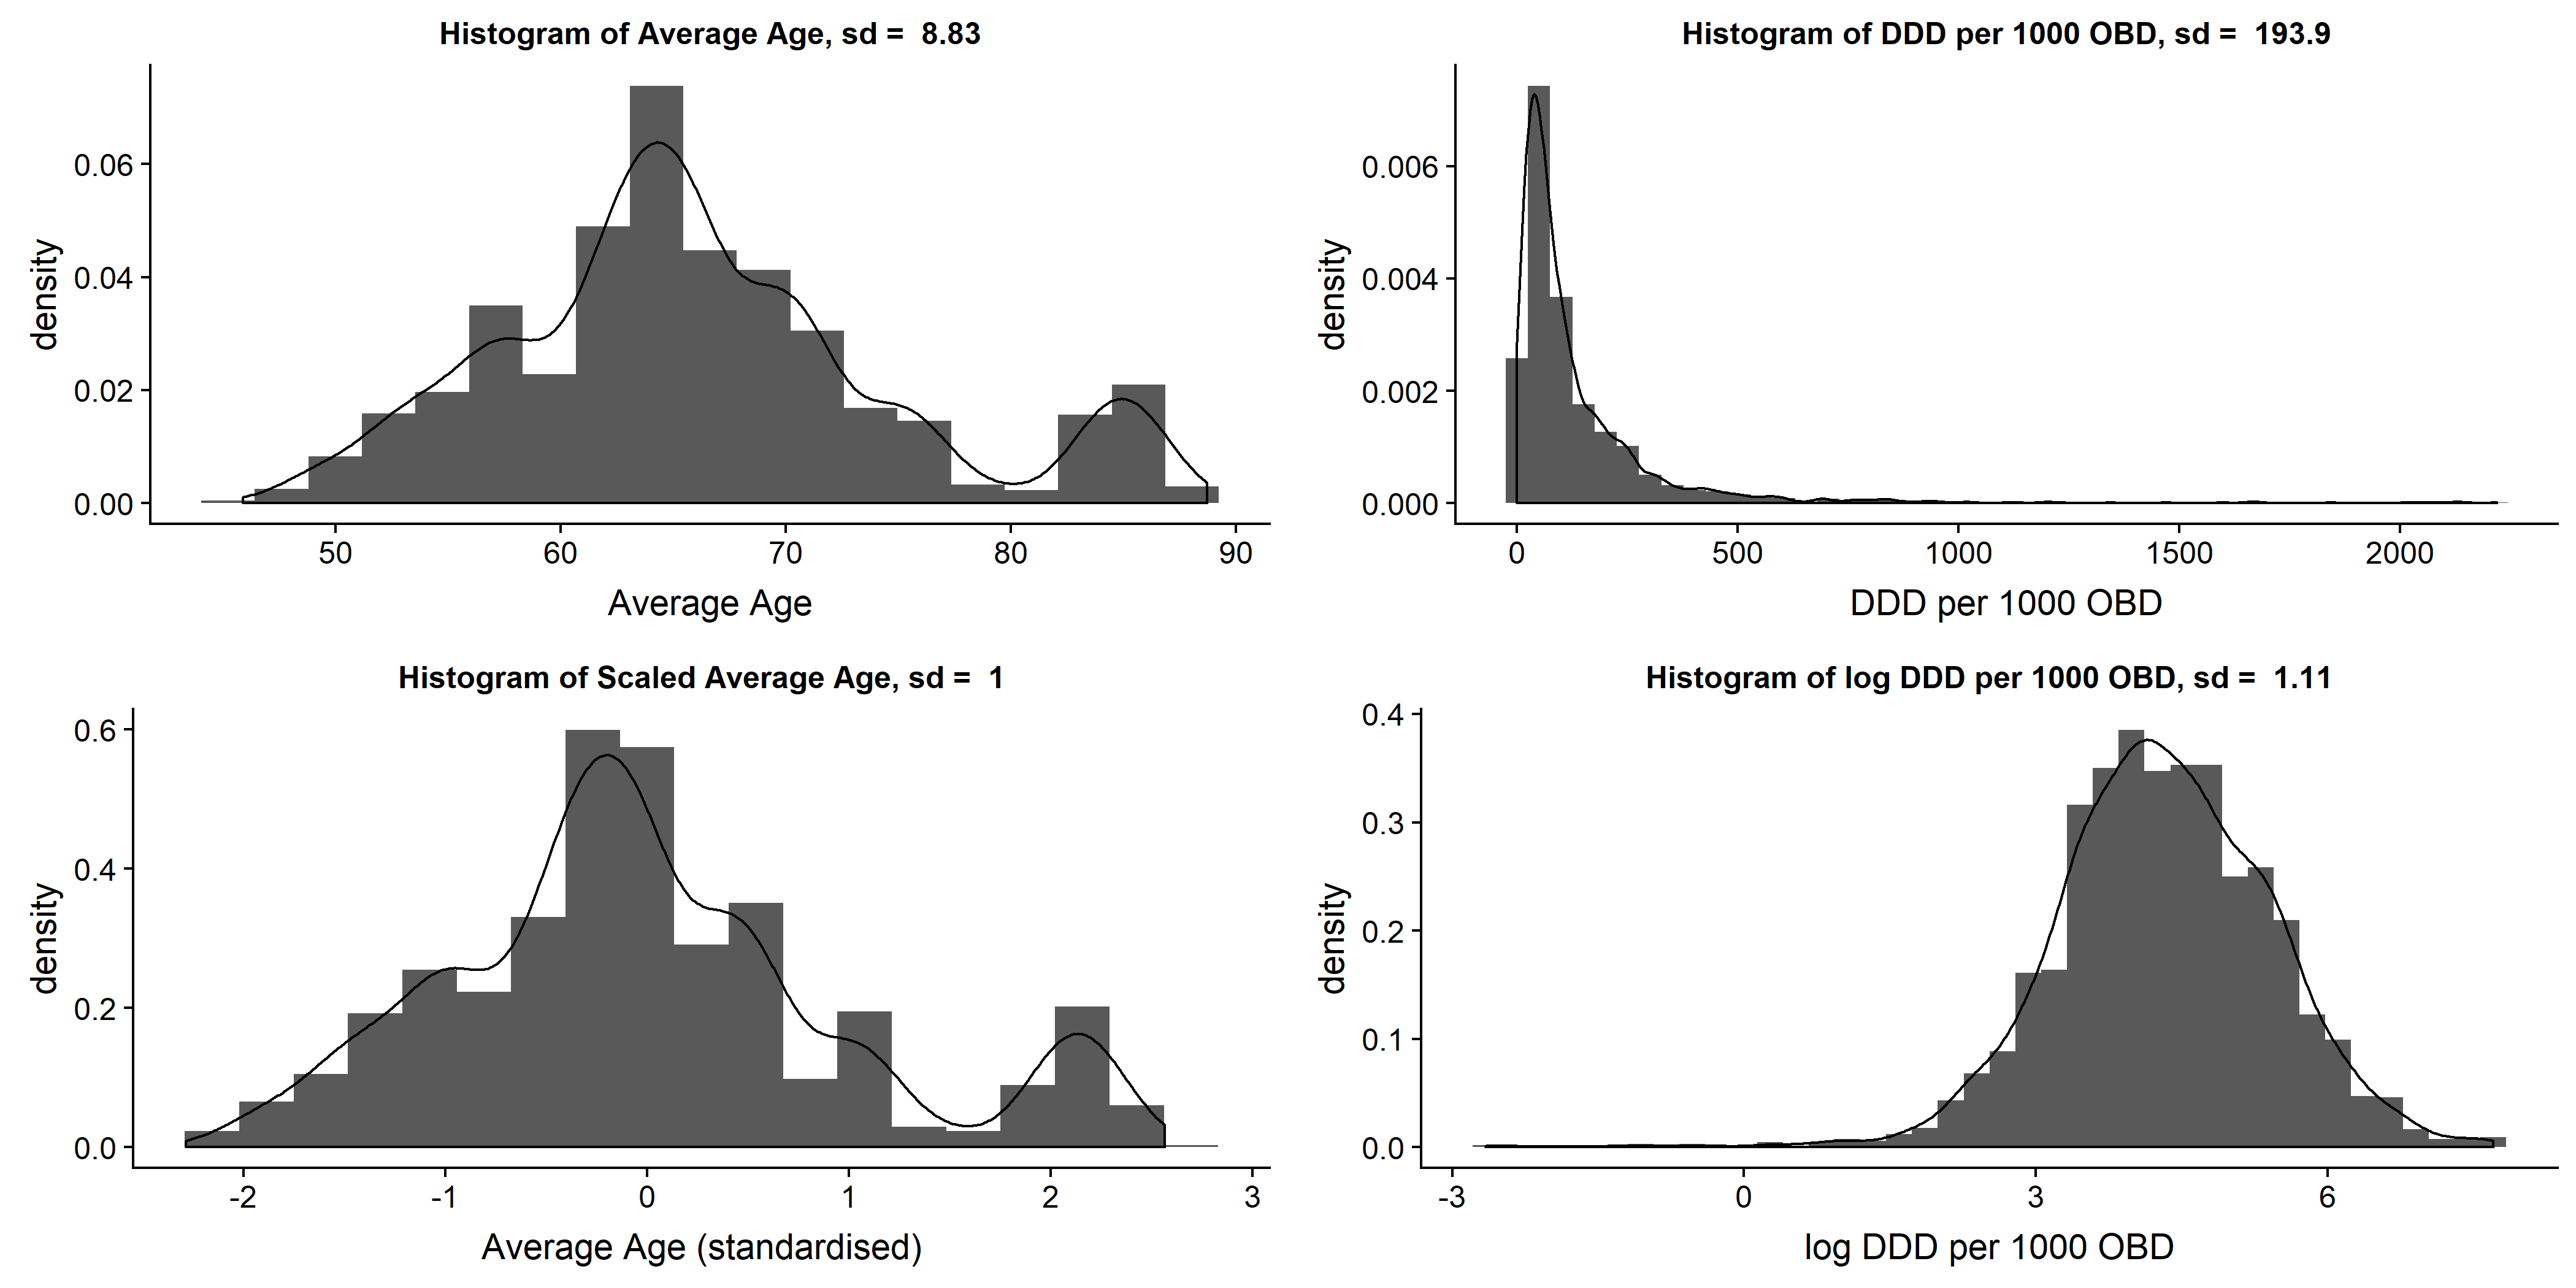
\includegraphics[width=\textwidth]{Figures/2_1_EDA_Cont.png}
\caption{Continuous Covariate Histograms} \label{fig::2_1_EDA_Cont}
\end{figure}

Figure \ref{fig::2_1_EDA_Fact} illustrates the relationship of proportion with factor variables, and the week. Red points signify the standard deviations, and annotated numbers refer to sample sizes. We see that non-invasive administration is associated with higher resistance, but no visible time trend.  

Some wards appear to have less resistance than others, however there is no natural grouping in the wards as all of the error bars (1 standard error) contain adjacent wards. 

Drug classes show separation into different groups based on the proportion. We group based on both observations, and proportion differences. For instance we group the top 2 classes as their means and errorbars overlap. However we do not include ``BL - Broad Pen" in the group as it has enough observations to be its own group. The groupings are shown in Table \ref{table::1}. This enables cleaner visualisation, and will be used as a starting point for modelling. 

An important feature is the volatility in the data, with standard deviations generally above 30\% for subgroups. This makes it difficult to generate good predictions on the data, as there is too much noise relative to the small dataset. 

\begin{figure}[h!]
	\centering
	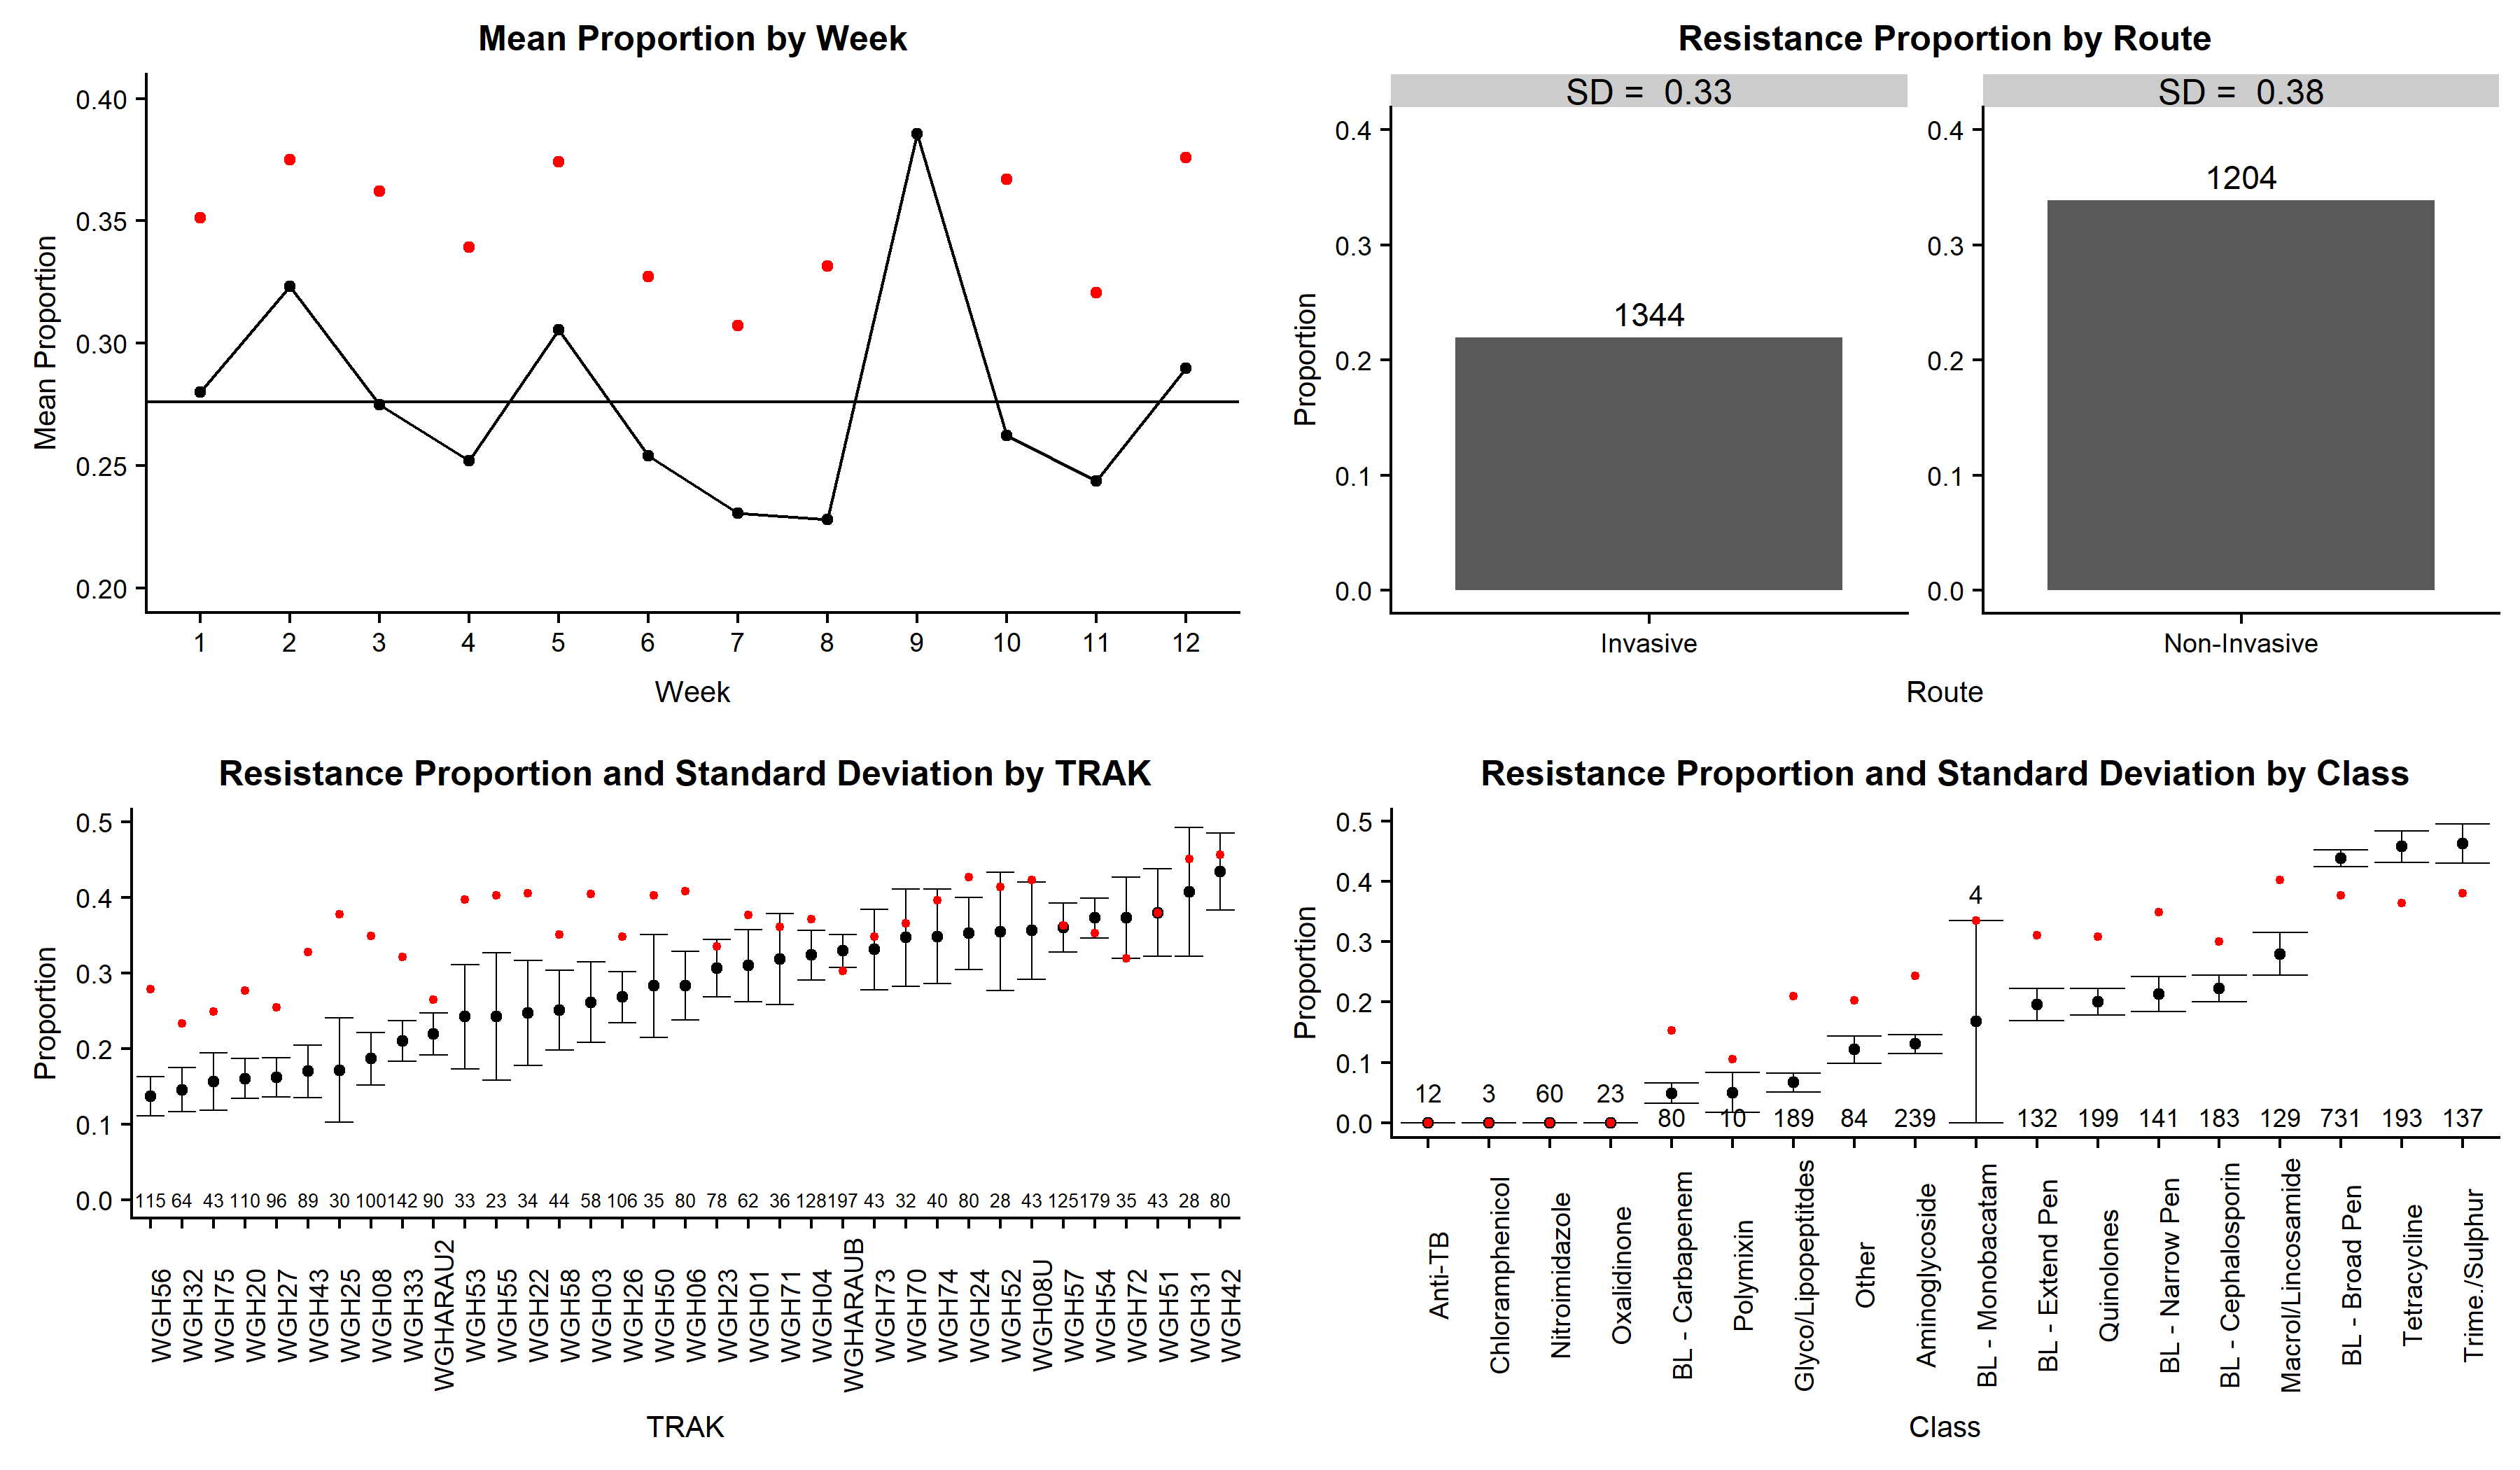
\includegraphics[width=1\textwidth]{Figures/2_1_EDA_Fact_Grid.png}
	\caption{Week and Discrete Covariates vs Proportion} \label{fig::2_1_EDA_Fact}
\end{figure}

\begin{table}[h!]
	\centering
	\begin{tabular}{|l|l|}
		\hline 
		Group & Drug Classes \\  \hline 
		A     & Anti-TB; Chloramphenicol; Nitroimidazole; Oxalidinone \\ 
		B     & $\beta$-Lactam - Carbapenem; Polymixin; Glycopeptides/Lipopeptides \\ 
		C     & Other; Aminoglycoside \\ 
		D     & $\beta$-Lactams (Extended Pen; Narrow Pen; Cephalosporin); Quinolones\\ 
		E     & Macrolide/Lincosamide  \\ 
		F     & $\beta$-Lactam - Broad Pen             \\ 
		G     & Tetracycline; Trimethoprim and sulphur based drugs \\ \hline
	\end{tabular} \caption{Drug Class Groupings}\label{table::1}
\end{table}

\newpage
Figure \ref{fig::2_1_EDA_Prop} visualises the proportion in 3 ways. The left panel exhibits a large number of 0s, 1s, and possibly 0.5s. This is clearer in the middle panel, which shows a frequency barplot for each \textit{individual} proportion. There are spikes at very specific values, such as 0, 1, 0.5, 0.25 and 0.33. As such, we can capture most of the shape in the proportion by grouping them into relevant intervals. This yields the barplot in the right panel, motivating the use of ordinal regression. 

\begin{figure}[!h]
	\centering
	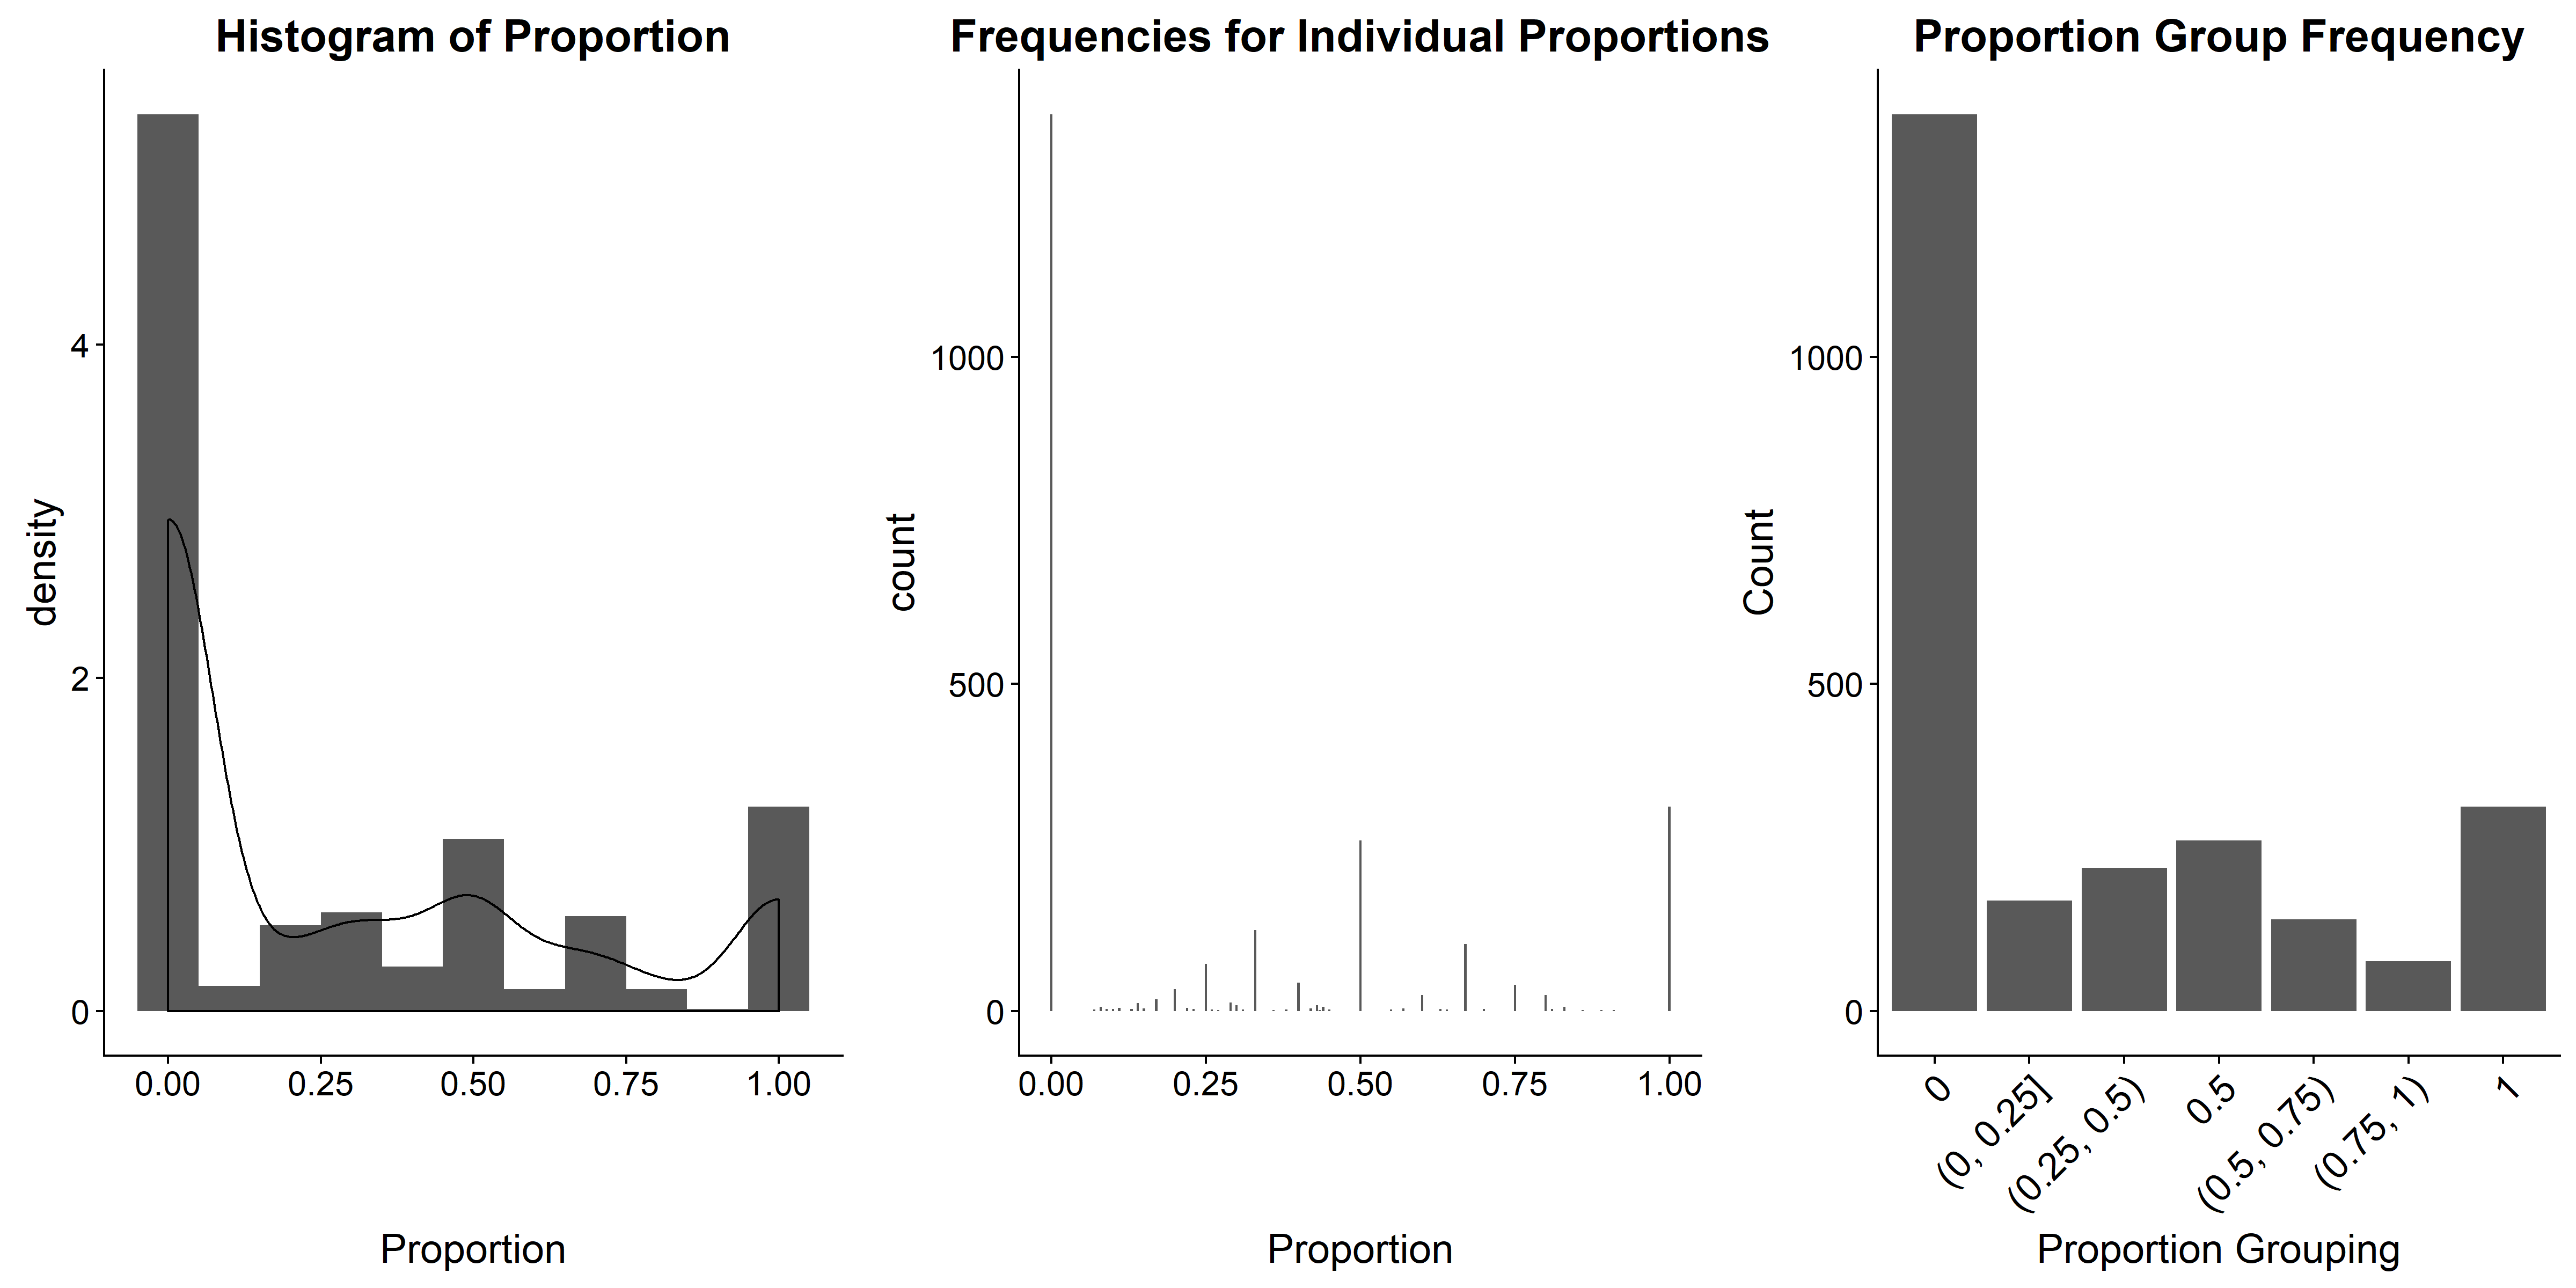
\includegraphics[width = 0.8\textwidth, height = 0.23\textheight]{Figures/2_1_EDA_Prop.png}
	\caption{Proportion Distribution} \label{fig::2_1_EDA_Prop}
\end{figure}

\subsection{Multiple Variables}

Recall that our interest is the association of DDD with resistance, so we include it in our model.   We will also include some sort of drug-specific effect -- the grouped class, raw class, or drug name -- based on the class-level proportion differences seen earlier. 


Figure \ref{fig::EDA_RouteProp} shows the estimated linear relationship between the proportion and the DDD, segmented by route. Invasively administered drugs seemingly have a lower resistance proportion for low levels of DDD, but increases in DDD have a stronger bearing on resistance than for non-invasively administered drugs. As such, we will include the route in our model, and interact it with age to account for the different slopes. 

\begin{figure}[h!]
	\centering
	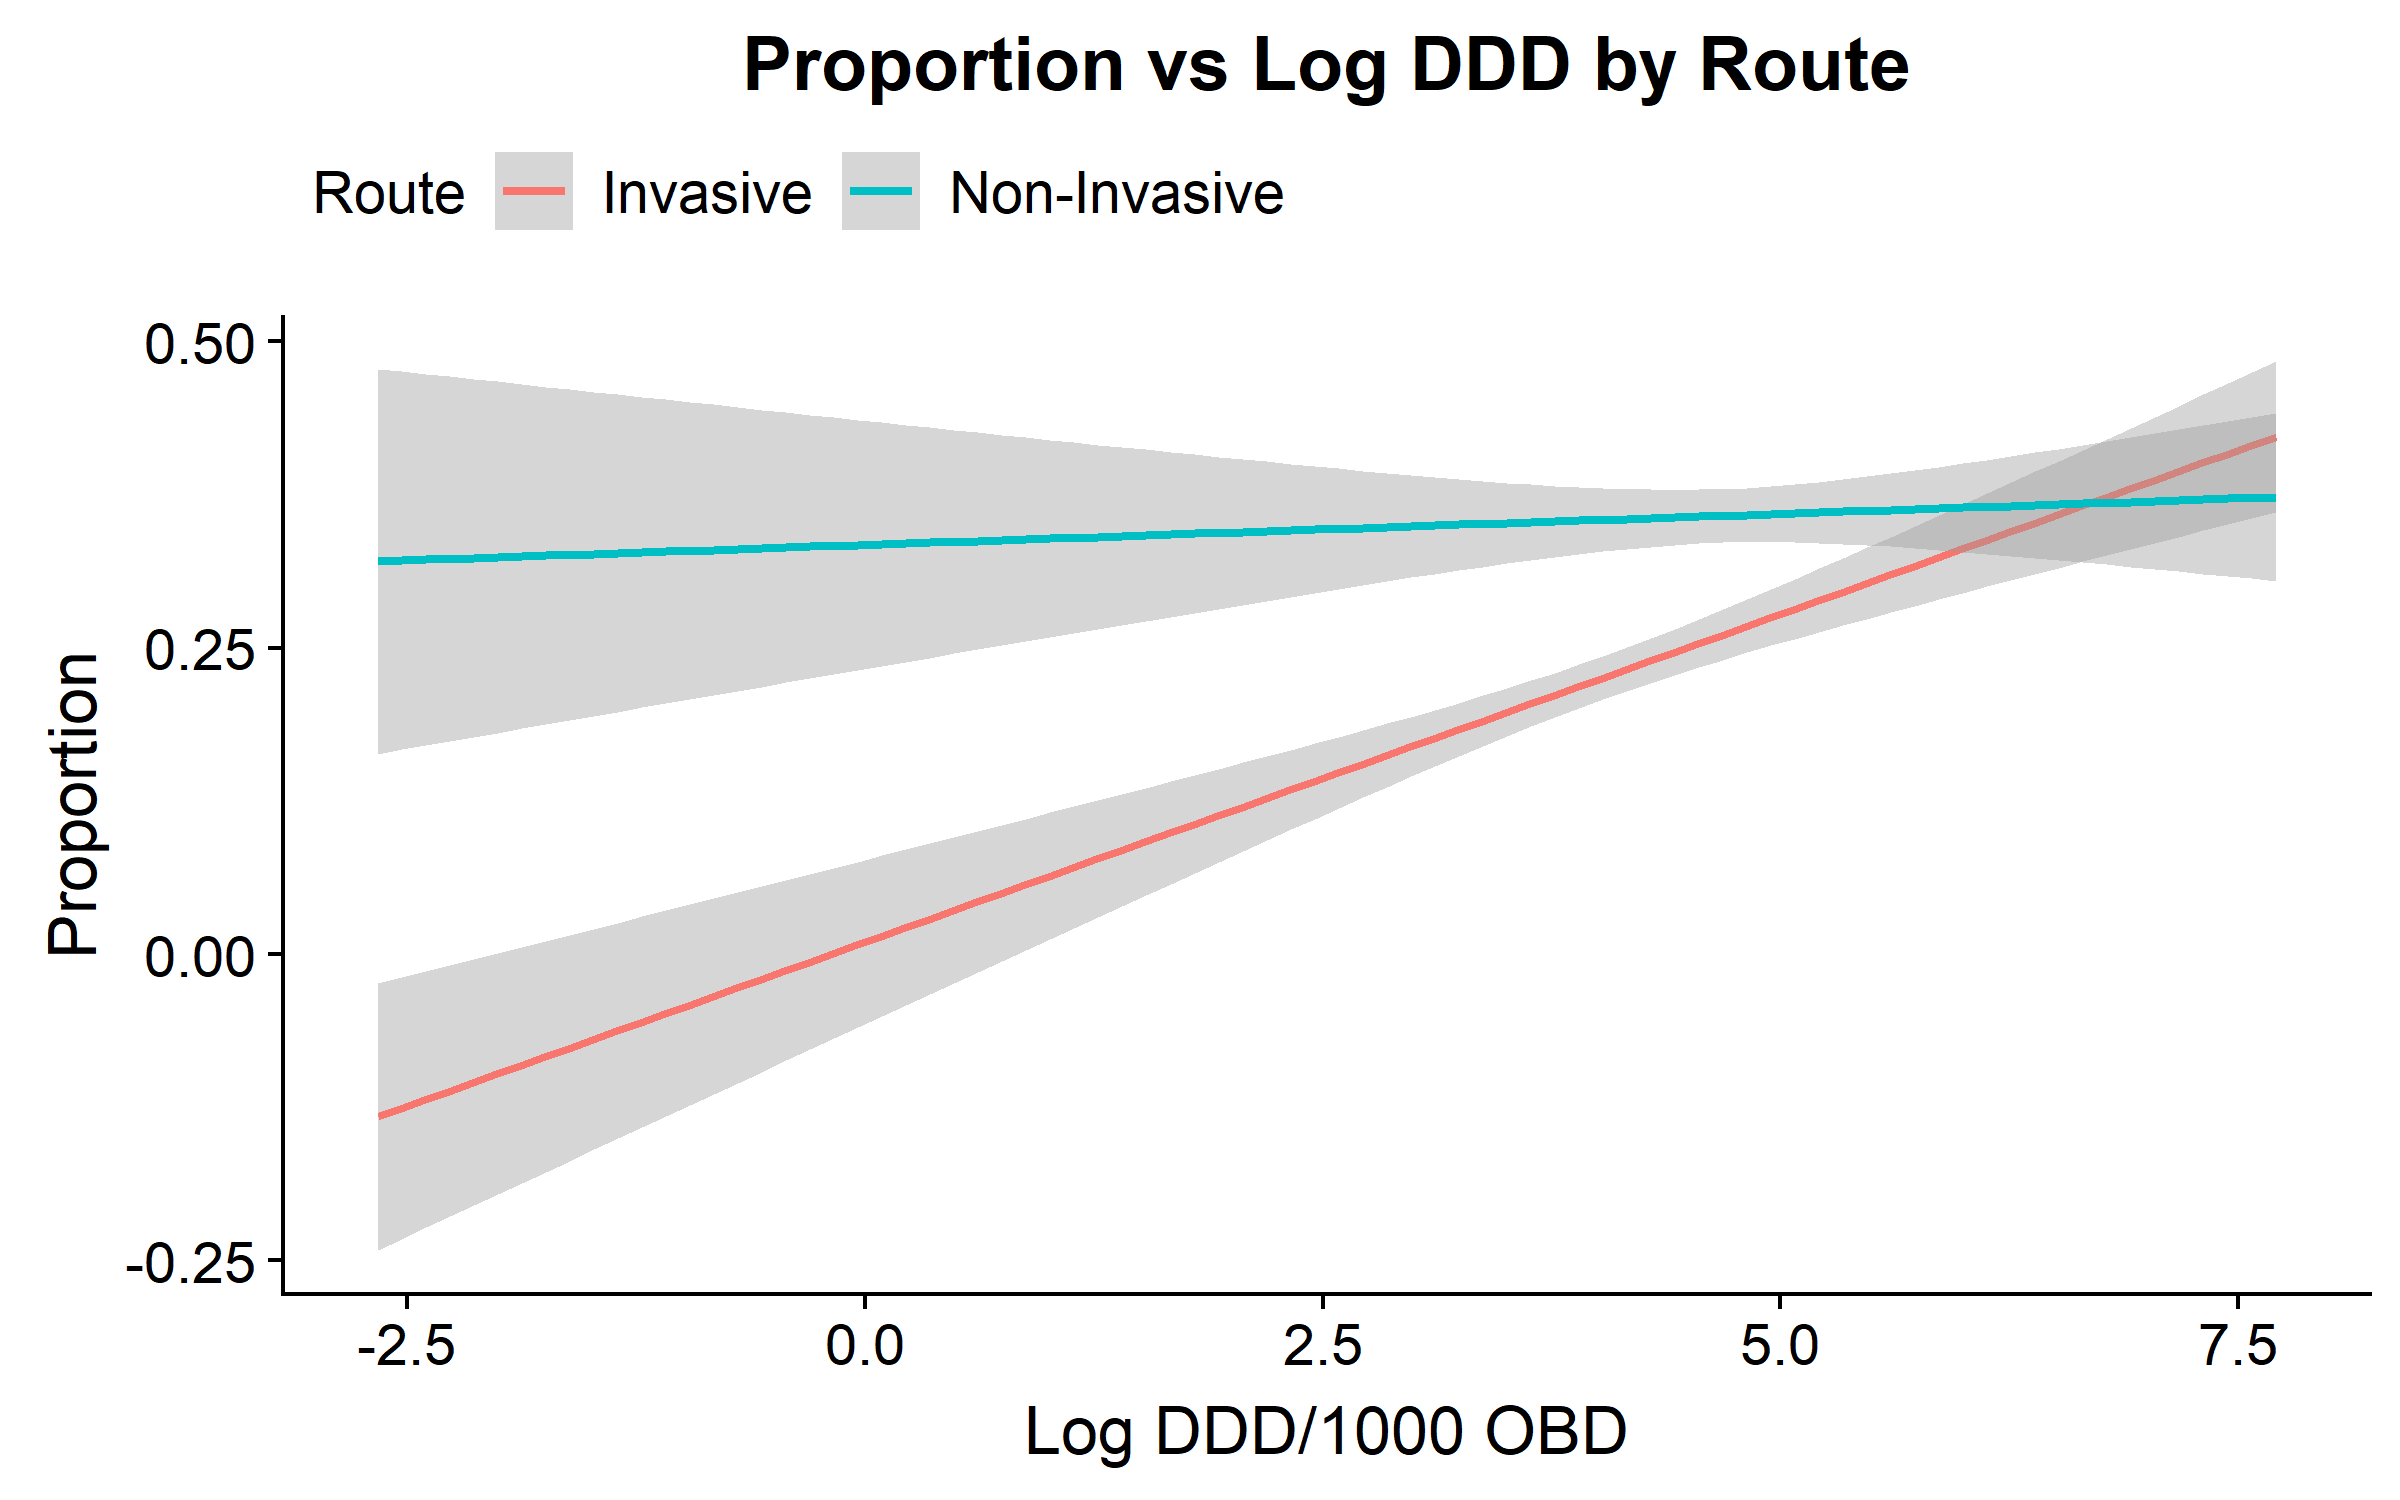
\includegraphics[height = 0.18\textheight]{Figures/2_5_1_EDA_RouteProp.png}
	\caption{Proportion-DDD Relationship by Route} \label{fig::EDA_RouteProp}	
\end{figure}

Figure \ref{fig::EDA_Age} suggests a negative relationship between age and DDD, which may be expected due to the increased sensitivity of the body to certain drugs in elderly patients as suggested in \cite{Hughes2002} and \cite{Turnheim1998}. This relationship slightly varies by class, but not enought to motivate varying slopes. Adjusted $R^2$ values range from 0 to 0.12 for each class, with all coefficients significant at the 5\% level except for group E. All slope coefficients were negative, ranging from -0.05 to -2.99. \\

We include age as a potential confounder, as it may have a direct influence on the proportion due to human-human resistance transmission (\citeauthor{Holmes2016}, \citeyear{Holmes2016}) in the elderly as a result of nursing homes. Age is therefore considered a potential ``fork" confounder as discussed in \cite{McElreath_book} and \cite{Pearl}. 

\begin{figure}[h!]
	\centering
	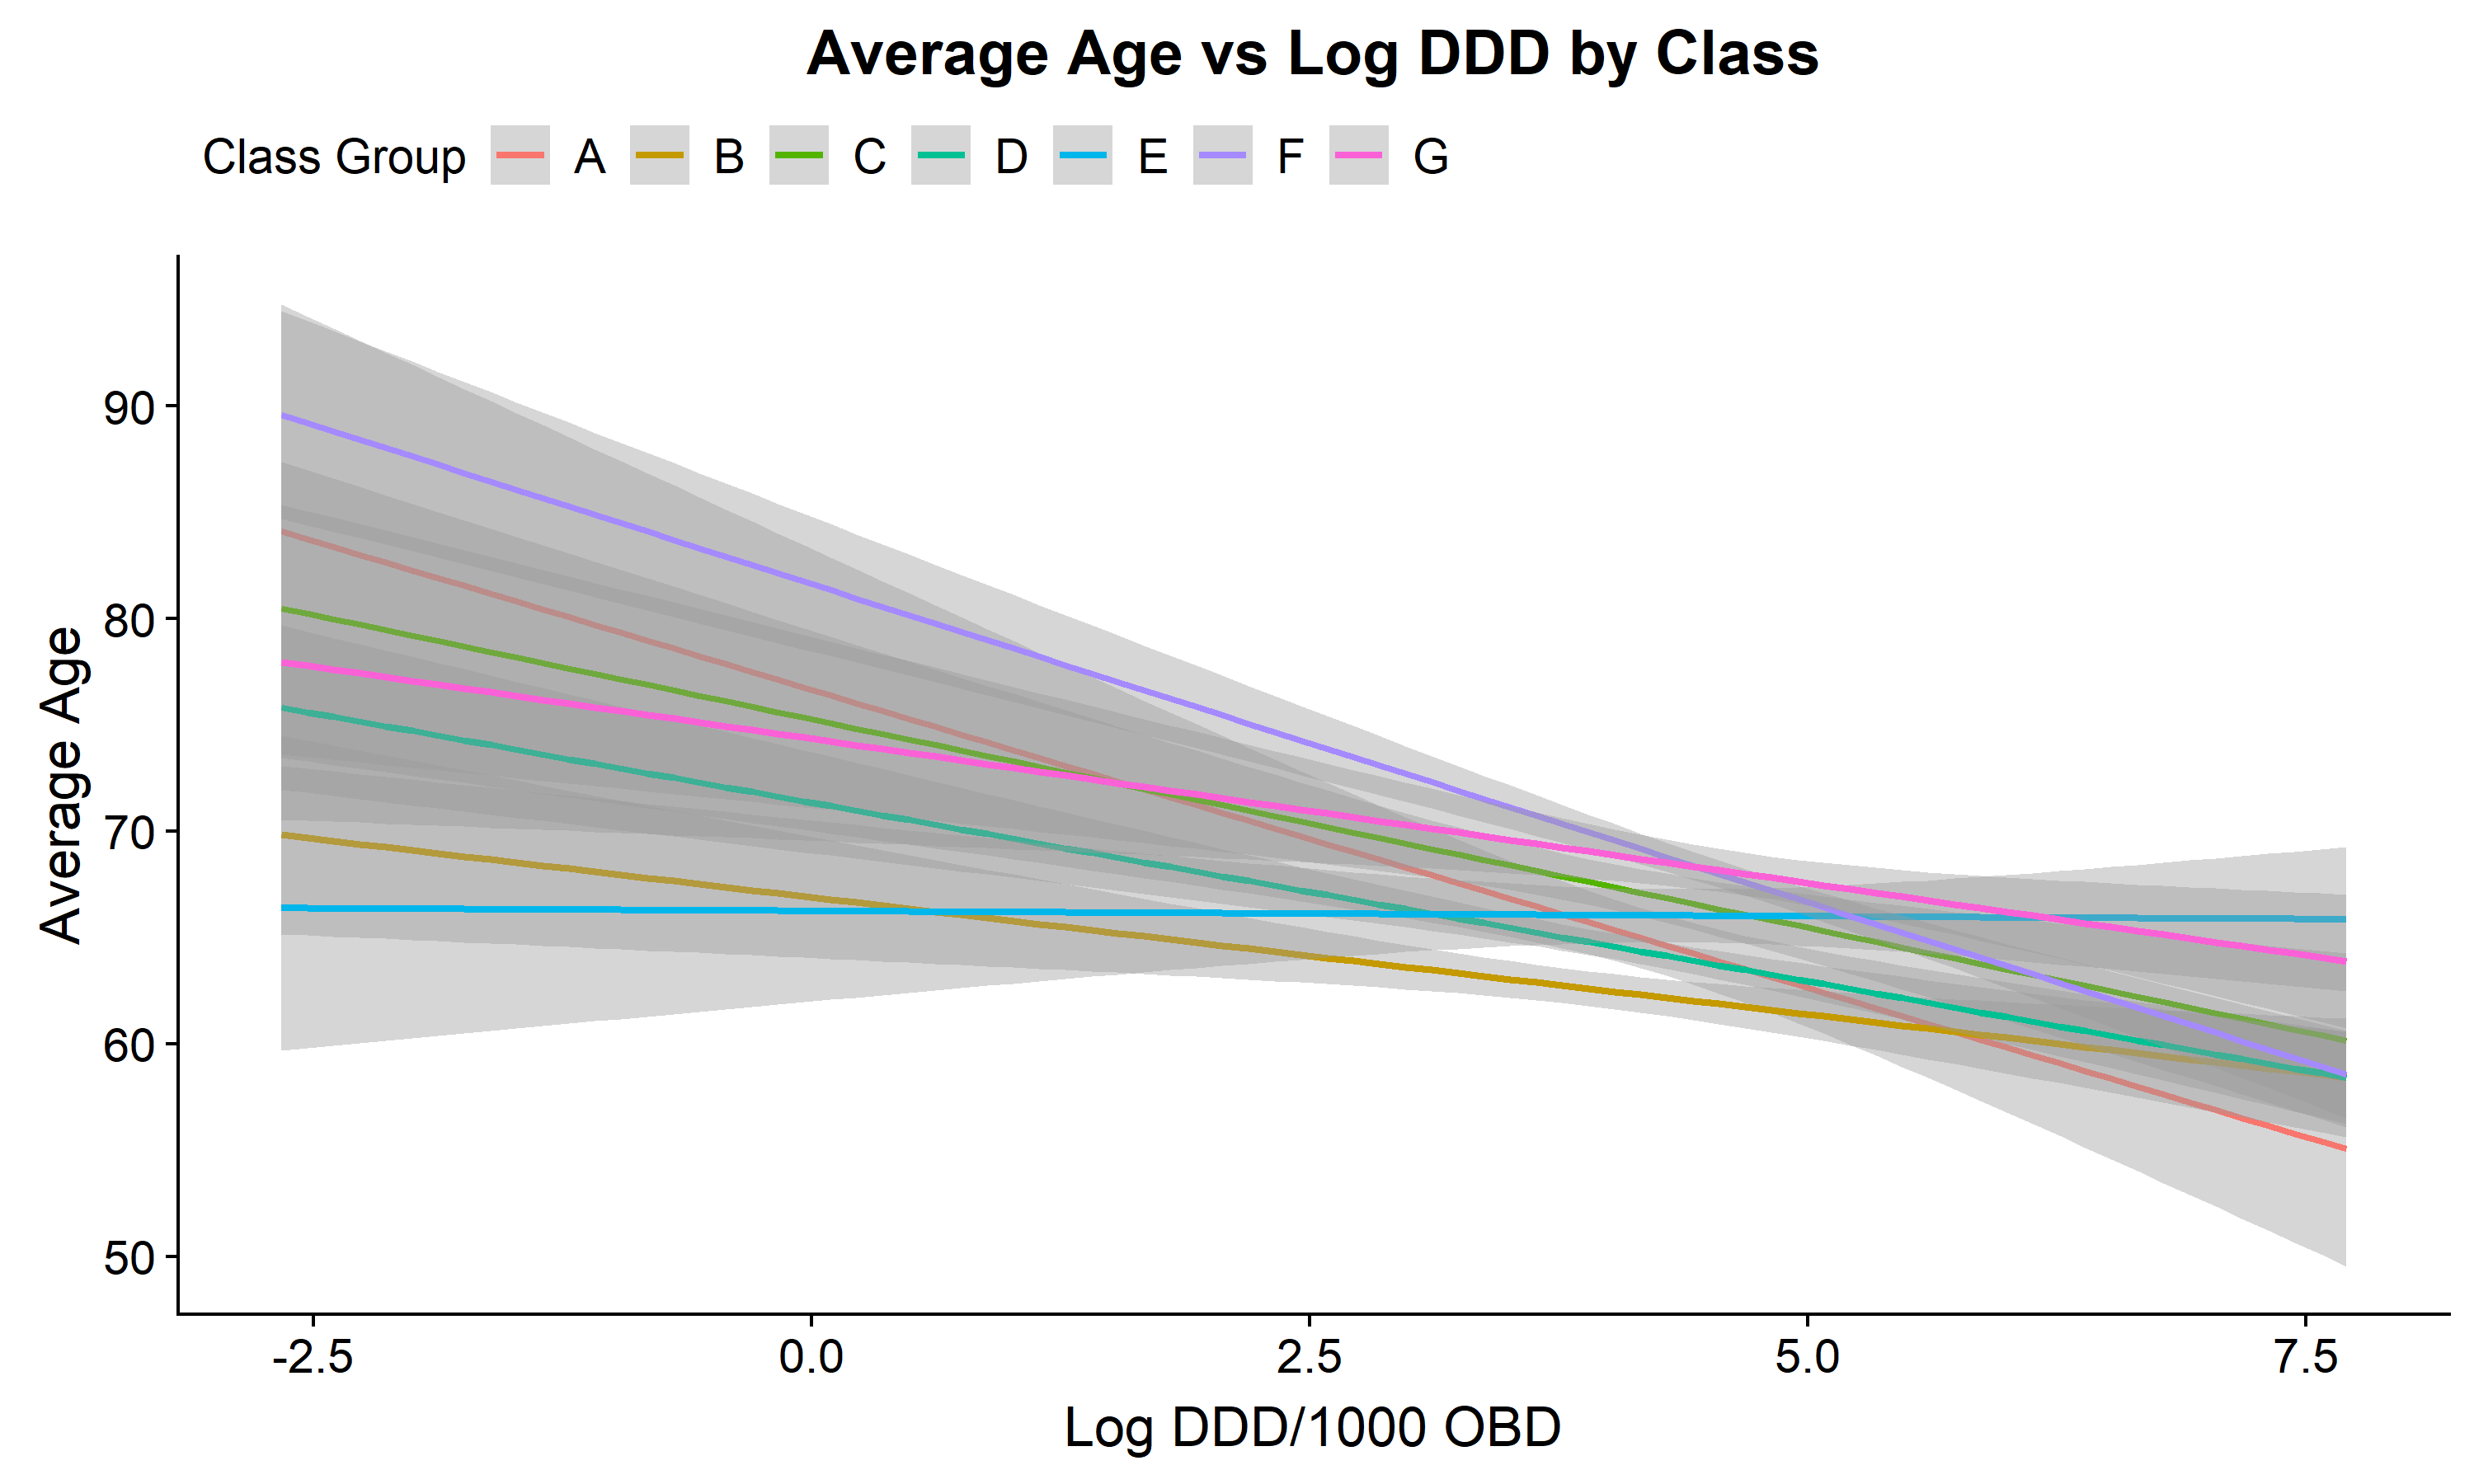
\includegraphics[height = 0.25\textheight]{Figures/2_4_1_EDA_Age.png}
	\caption{Age-DDD Relationship by Class Grouping} \label{fig::EDA_Age}	
\end{figure}


Figure \ref{fig::EDA_ClassDDDSlope} shows a slight positive slope for groups B, C, and D but flat slopes for E, F, and G. However due to the level of variation in the confidence intervals and the small differences, we posit population-level effects, as any group-level effects will be too subtle with our noisy data.  

\begin{figure}[h!]
	\centering
	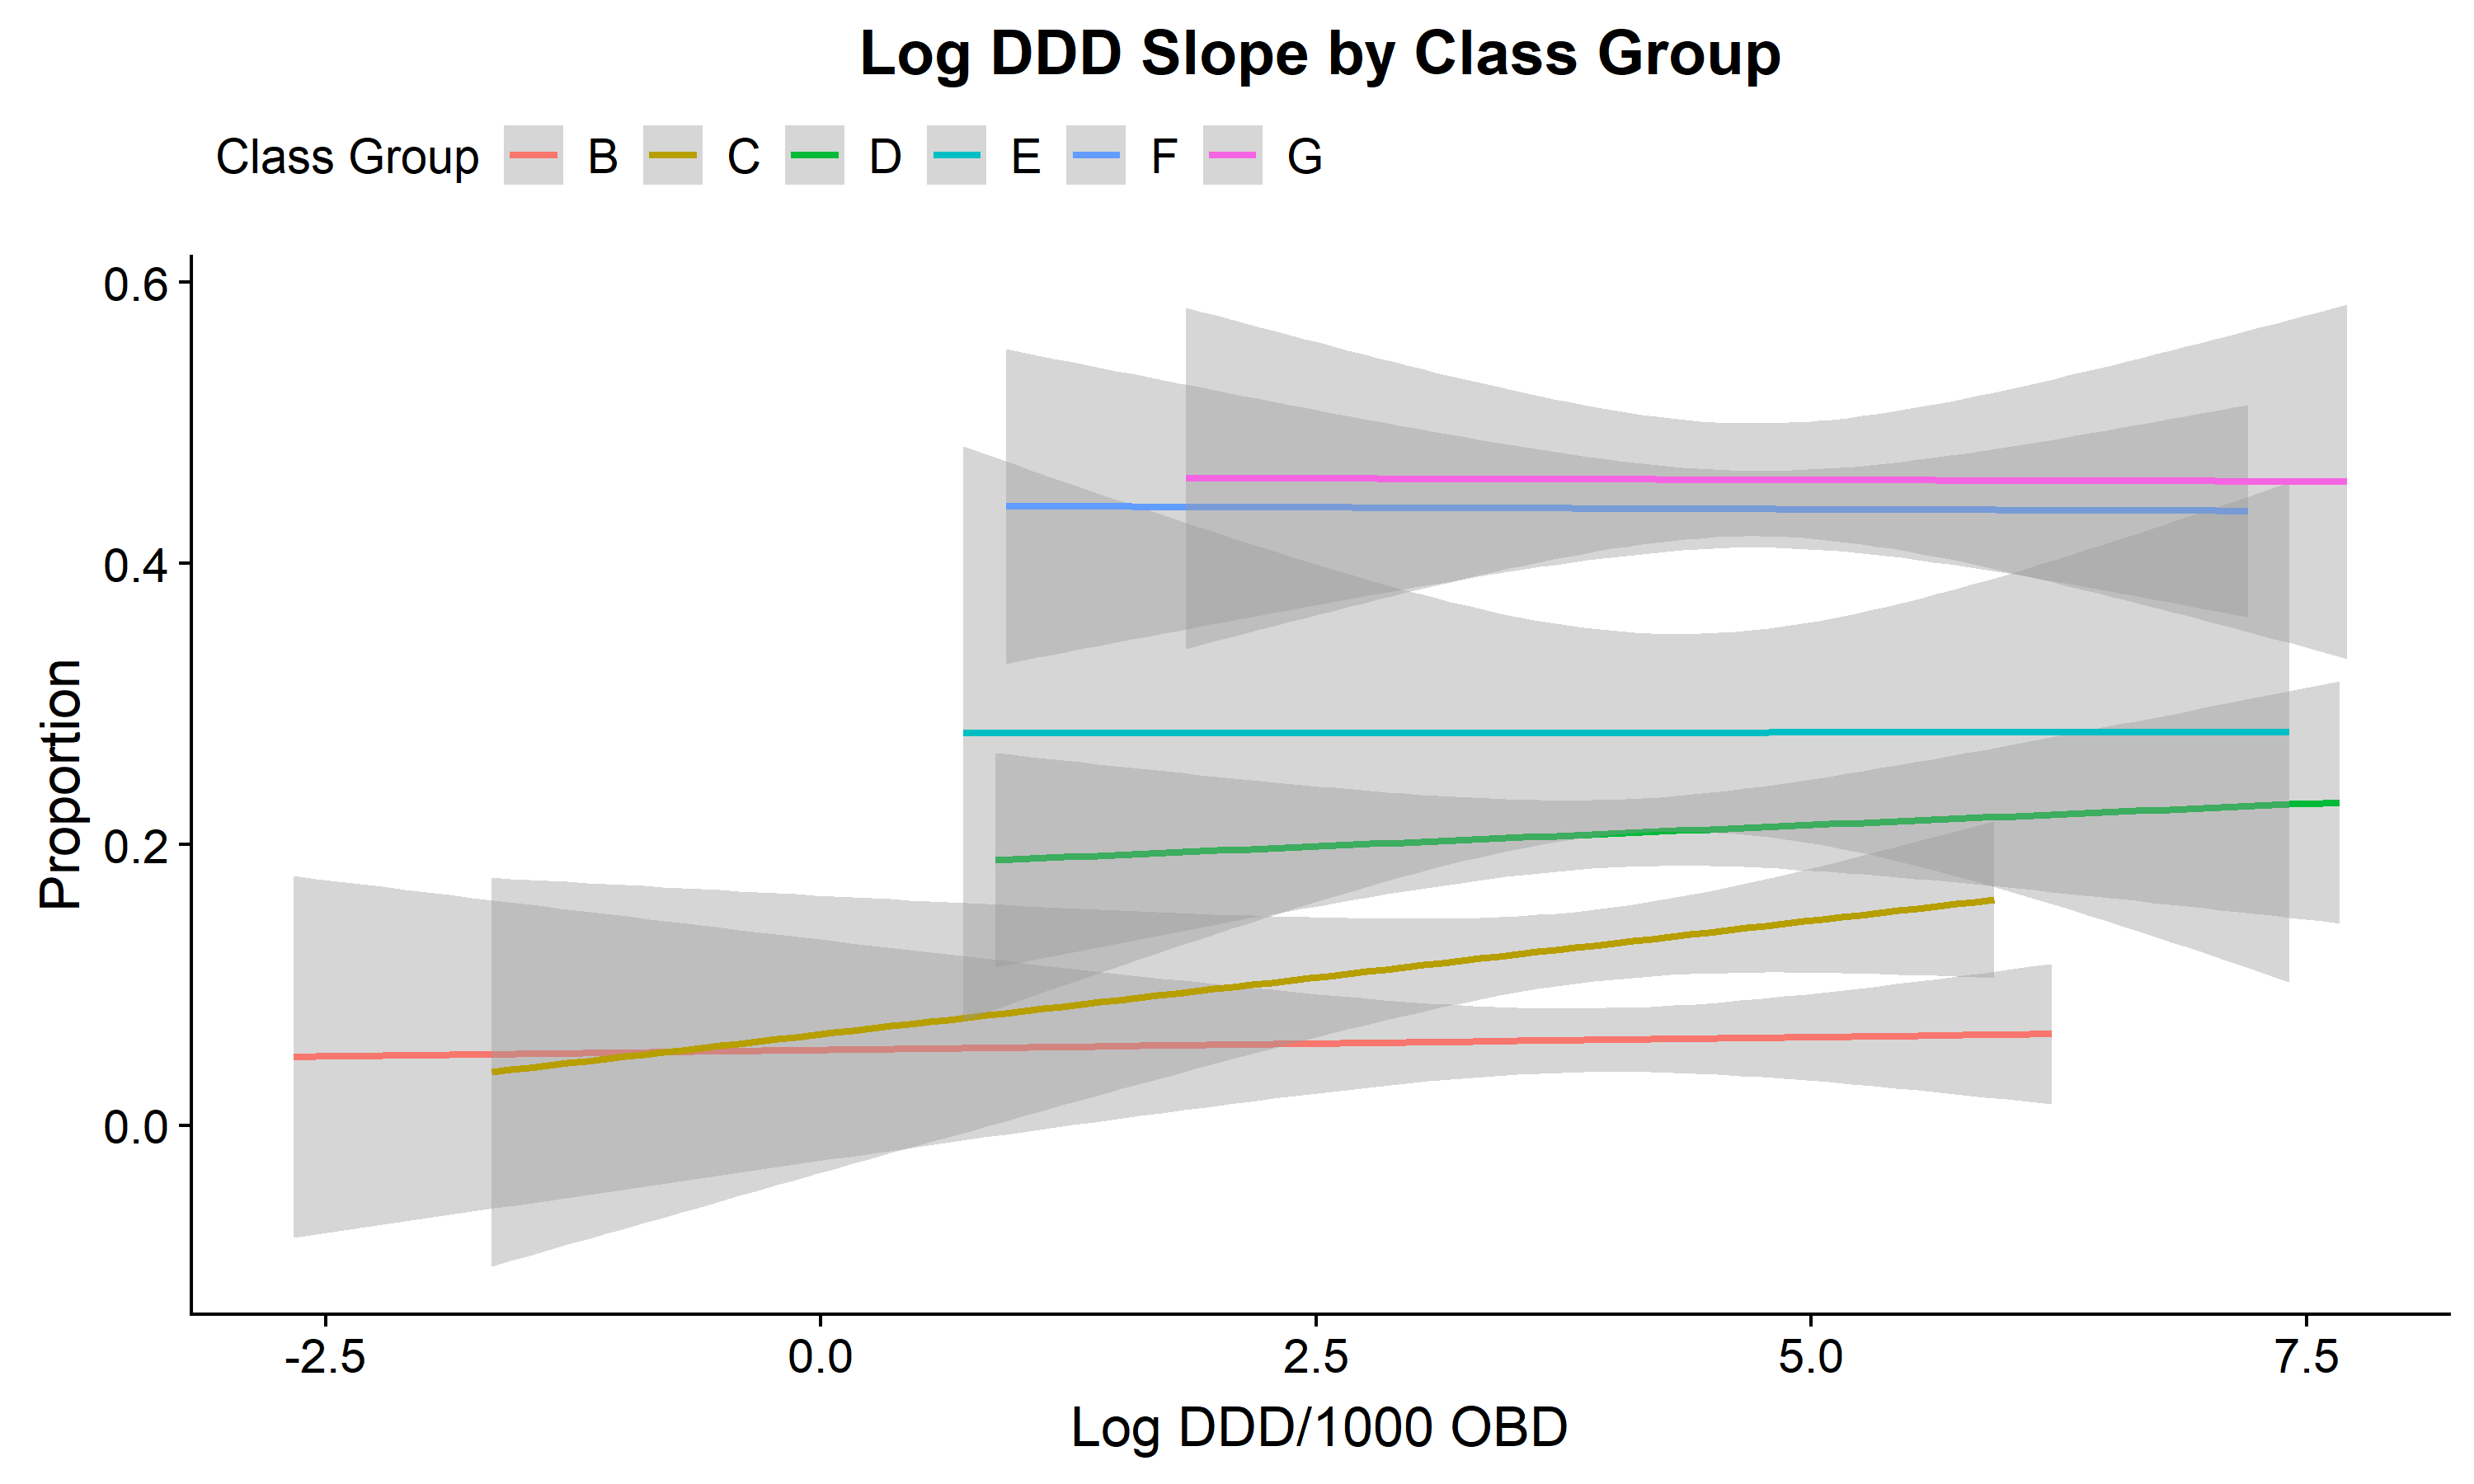
\includegraphics[height = 0.25\textheight]{Figures/2_2_EDA_ClassDDDSlope.png}
	\caption{DDD-Proportion Relationship} \label{fig::EDA_ClassDDDSlope}	
\end{figure}

Figure \ref{fig::EDA_ClassWeek} suggests that the week has little influence on the proportion. There is a downward slope for group E, however there is a large degree of variation. Therefore we consider week to have no effect on the proportion. 

\begin{figure}[h!]
	\centering
	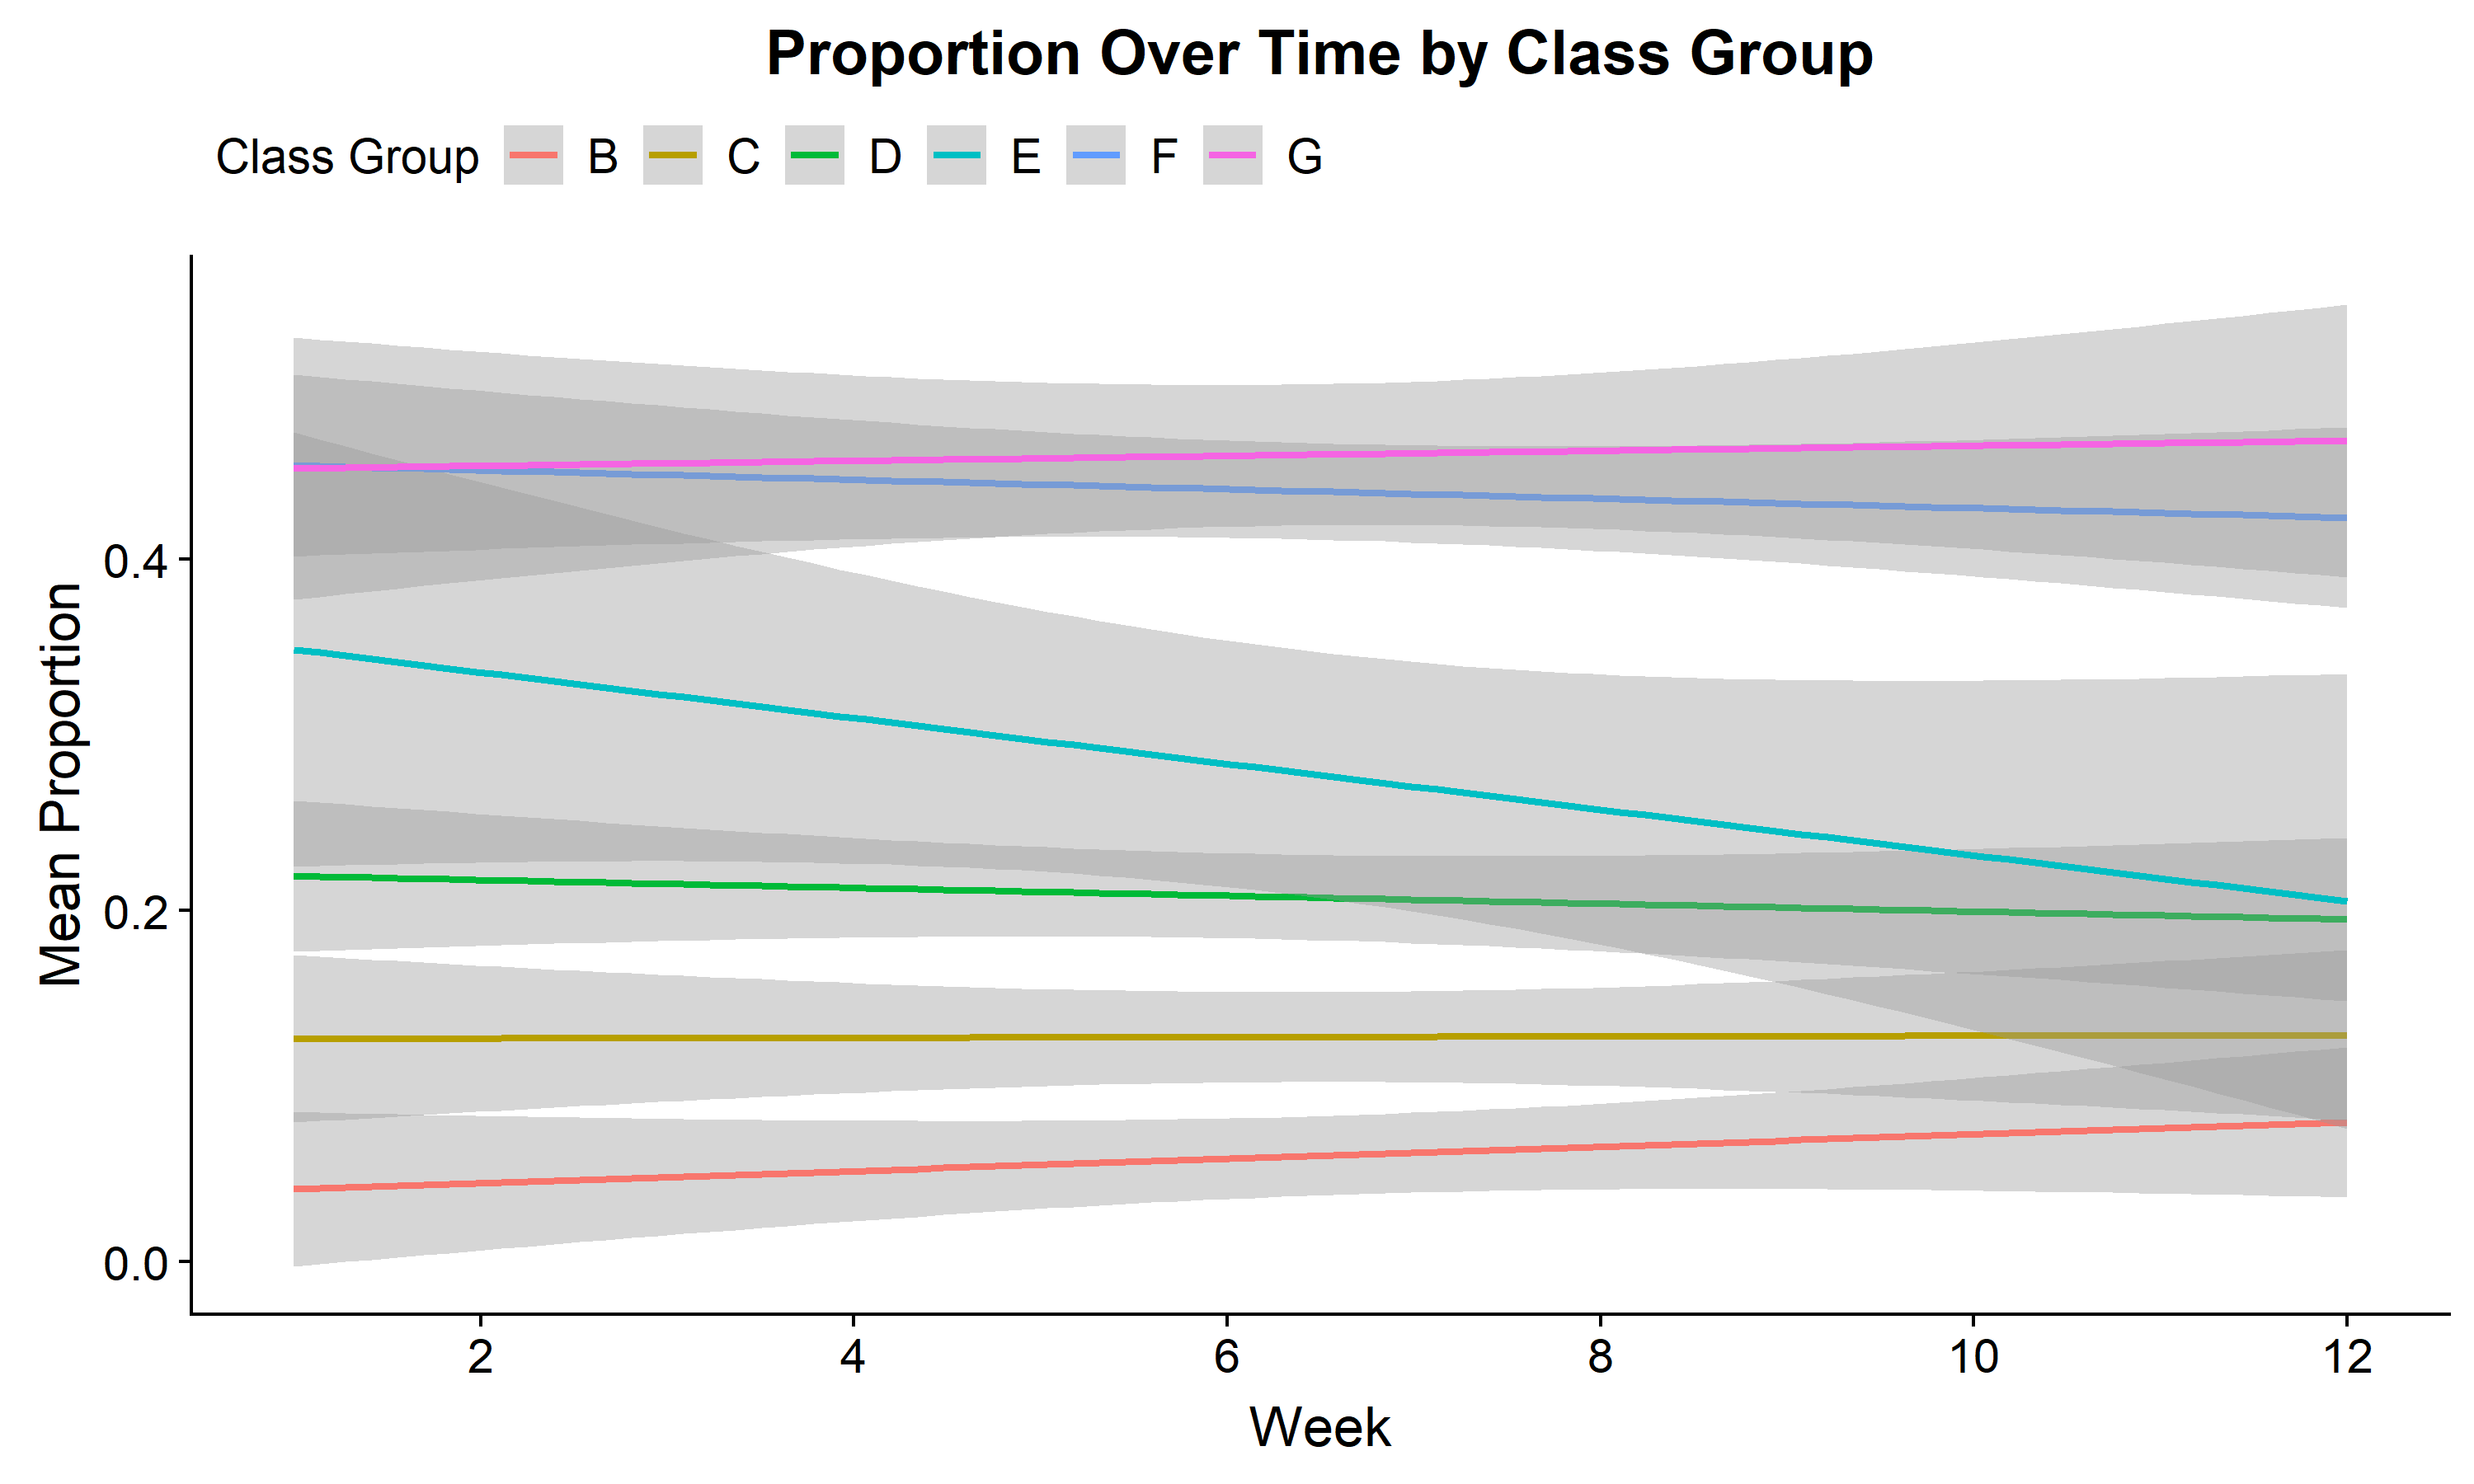
\includegraphics[height = 0.25\textheight]{Figures/2_2_EDA_ClassWeek.png}
	\caption{Proportion over time by Class Group} \label{fig::EDA_ClassWeek}	
\end{figure}

Figure \ref{fig::EDA_TRAKAge} points to a strong relationship between the age and the ward, with the ward seemingly a good predictor of the age due to the low age variation within most wards. A linear regression of age on TRAK yields an adjusted $R^2$ of 0.9329, suggesting including both TRAK and age would be redundant. We select age for theoretical reasons, and to avoid including too many parameters.

\begin{figure}[h!]
	\centering
	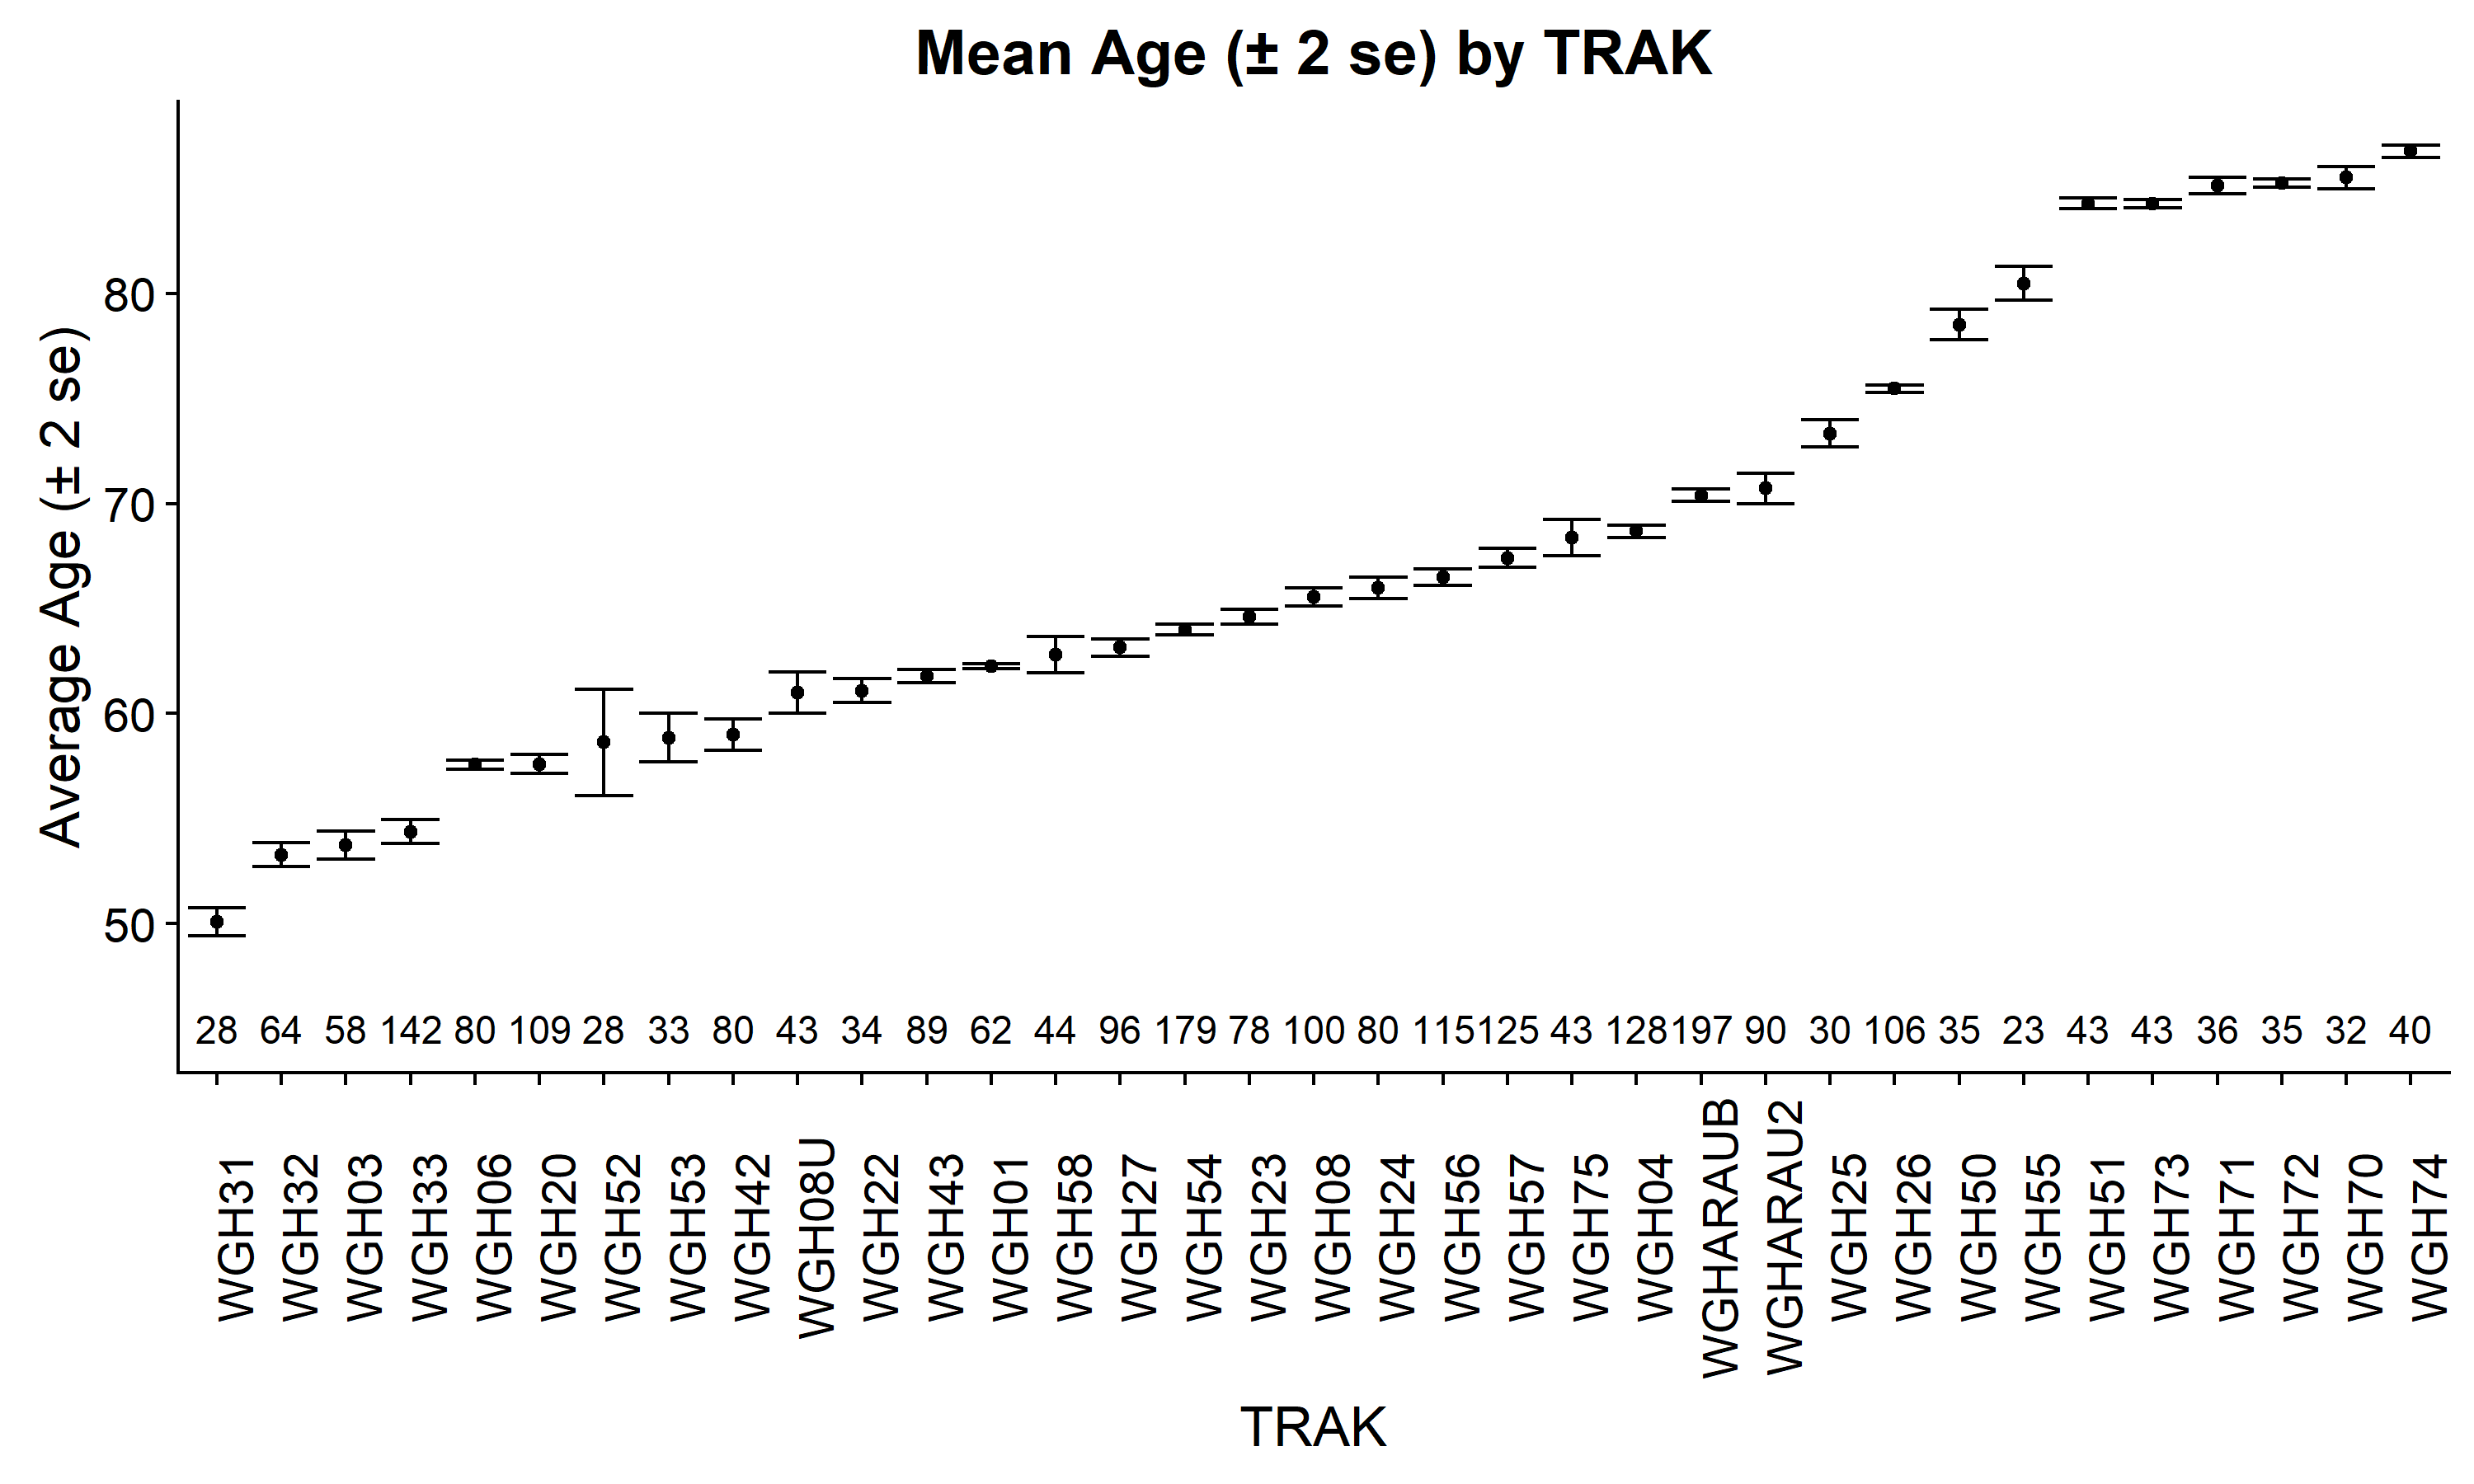
\includegraphics[height = 0.35\textheight]{Figures/2_3_1_EDA_TRAKAge.png}
	\caption{TRAK-Age Relationship} \label{fig::EDA_TRAKAge}	
\end{figure}

\clearpage


\subsection{EDA Summary}

We have

\begin{enumerate}
	\item Transformed the proportion to a set of ordered groups. 
	\item Grouped drug classes based on their level of resistance for initial modelling.  
	\item Standardised the average age, and logarithmised the DDD/1000 OBD. 
	\item Decided to include log DDD as a population level effect, with an interaction on the route. 
	\item Included age as a population-level effect
	\item Not included week due to a lack of any visible relationship in the data. 
	\item Not included TRAK due to its strong relationship with age. 
\end{enumerate}

\newpage

\section{Model} \label{sec::Model}

We use a Bayesian ordered logit with varying intercepts. This section provides an overview of ordered logit, discusses the latent variable, and specifies our priors.

\subsection{Ordered Logit}

This subsection gives an overview of ordered logit. Options for a more comprehensive treatment include \cite{WalkerDuncan1967Logit, McCullagh1980}, and \cite{Greene2012} (ordered probit).

In ordered logit, our response variable is the binned proportion ($y$). Ordinal regression supposes there is a latent variable ($y^* \in \mathbb{R}$) which leads to our bins by the process below. We have thresholds $c_j, j \in \{0, 1, \dots K = 7\}$, where $c_0 = -\infty$, and $c_7 = \infty$. 

\[
y = 
\begin{cases}
0 & \text{if } y^*            \in (-\infty, c_1]\\
(0, 0.25] & \text{if } y^*    \in (c_1, c_2]\\
(0.25, 0.5) & \text{if } y^*  \in (c_2, c_3]\\
0.5 & \text{if } y^*          \in (c_3, c_4]\\
(0.5, 0.75] & \text{if } y^*  \in (c_4, c_5]\\
(0.75, 0.99) & \text{if } y^* \in (c_5, c_6]\\
1 & \text{if } y^*            \in (c_6, \infty)\\
\end{cases}
\]


For the cumulative logit, we assume the latent variable follows a logistic distribution with scale 1 (variance $\frac{\pi^2}{3}$) and mean $\eta$ (the usual linear predictor $\mathbf{x}'\beta$, excluding the intercept). We define the cumulative distribution function (CDF) of the standard logistic distribution as $\Lambda$. 

\begin{align*}
	y^* &\sim Logistic(\eta, 1) \\
	\Lambda(x) &= \frac{exp(x)}{1 + exp(x)}
\end{align*}


\begin{figure}[h]
	\centering
	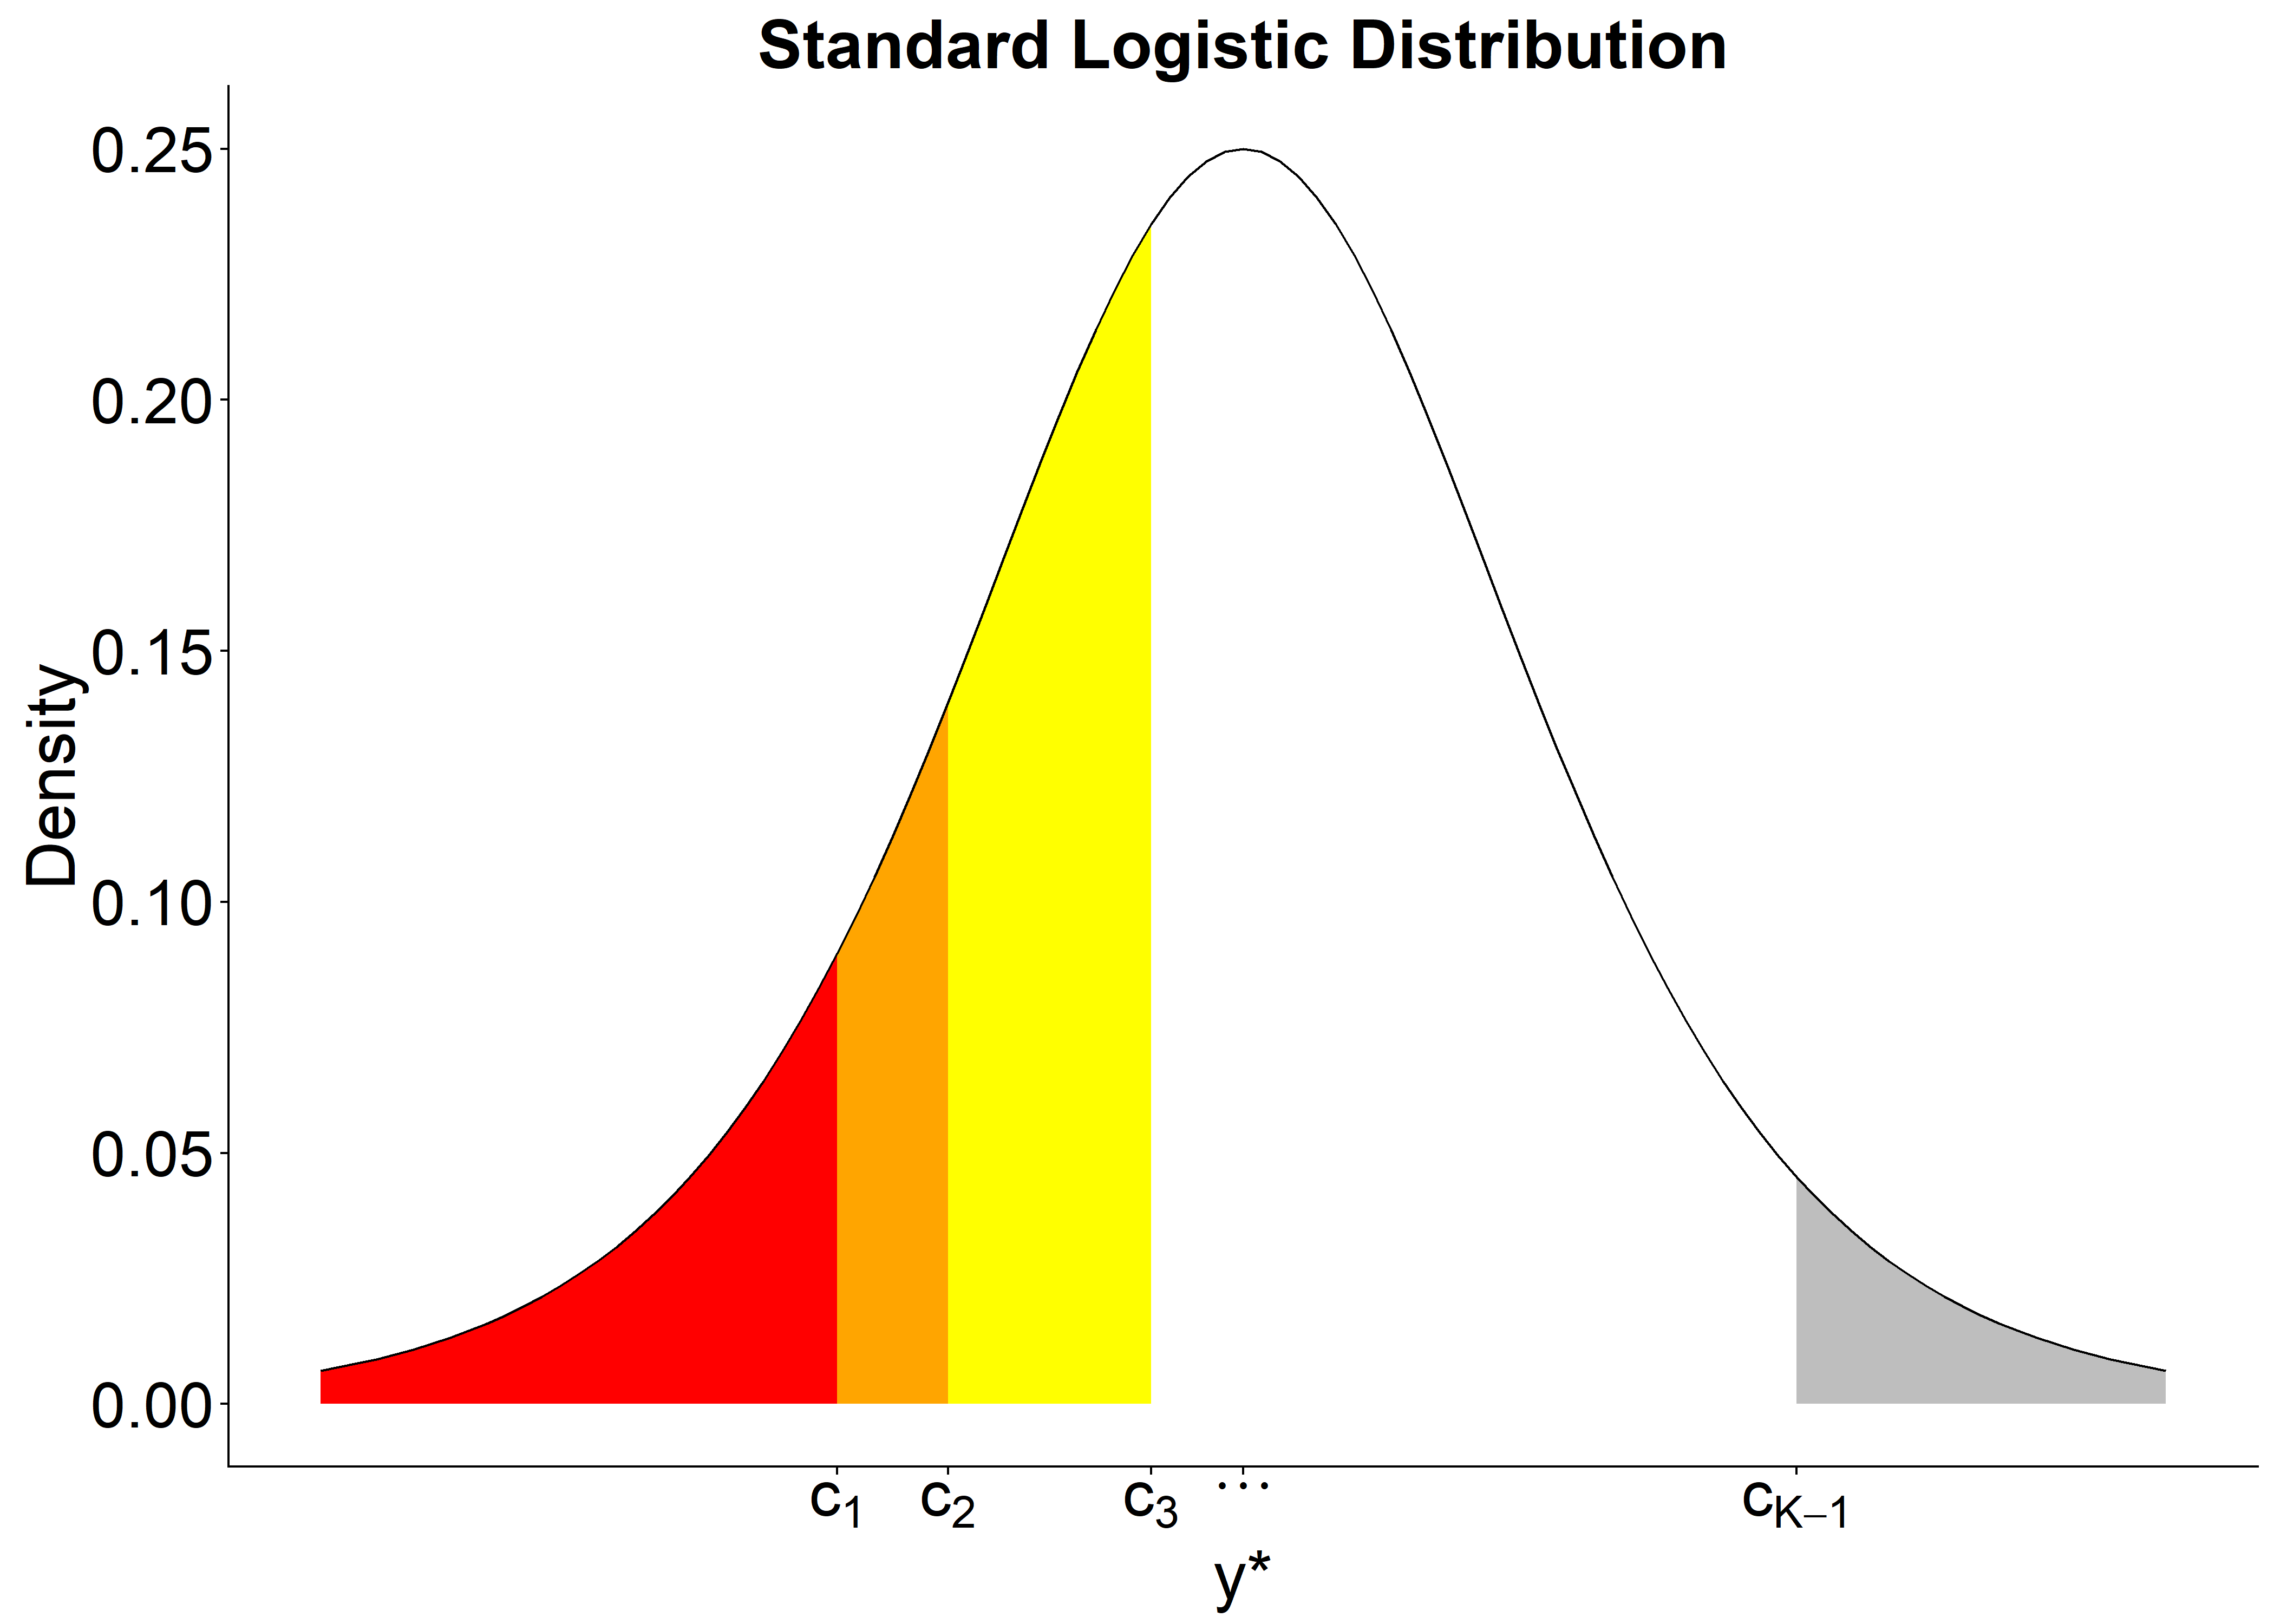
\includegraphics[height = 0.3\textheight]{Figures/0_Logit.png}
	\caption{Latent Variable Categorisation} \label{fig::0_Logit}
\end{figure}


The probability $y$ is in category k given $\eta$ is $Pr(y = k) = Pr(y^* \in (c_{k-1}, c_{k}))$ $= \Lambda(c_k- \eta) - \Lambda(c_{k-1} - \eta)$. This concept is illustrated in Figure \ref{fig::0_Logit}. For example, the yellow region is the probability the latent variable is between $c_2$ and $c_3$, i.e. the probability of the observed category being category 3. We therefore define the pdf and likelihood as:

\begin{align}
f(y) &= \prod_{j = 1}^{K}[\Lambda(c_j - \eta) - \Lambda(c_{j-1} - \eta)]^{I(y=j)}  \\
L &= \prod_{i=1}^{n} \prod_{j = 1}^{K}[\Lambda(c_j - \eta_i) - \Lambda(c_{j-1} - \eta_i)]^{I(y_i=j)} 
\end{align}

Where $\eta_i$ refers to covariates changing by observation. 

Define $\gamma_j = Pr(y^* \le c_j)$. We then have $\gamma_j = Pr(y^* \le c_j) = \Lambda(c_j - \eta)$.  Applying $\Lambda^{-1}$:

\begin{align}
	\Lambda^{-1}(\gamma_j) &= logit(\gamma_j) = log\left(\frac{\gamma_j}{1 - \gamma_j}\right) = c_j - \eta \label{eq::logitlink}
\end{align}

We can interpret the coefficients in $\eta$ in relation to the log odds. Suppose $\beta_1 > 0$ is the coefficient on $x_1$. A one unit increase in $x_1$ increases the log-odds of a higher category by $\beta_1$. This interpretation is independent of the category, which is where ``proportional odds" comes from. 

\subsection{Resistance Score as the Latent Variable} \label{sec::3_Latent}

It may be concerning that we know the bins were created using the proportion, which is non-logistic. The application of ordered logit therefore requires a level of abstraction. We posit an underlying ``resistance score" that is impossible to measure, but can be partially captured by the proportion. Our latent variable is mapped to the proportion, which we transform to our bins. We suppose there is a function $f$ which maps from the reals to the closed interval [0,1]. Additionally, there is a function $g$ which maps from the interval $(c_1, c_{K-1})$ to the open interval (0,1). We define $f$ below, along with a mathematical statement of the function mappings. 

\begin{align*}
f: &\mathbb{R} \mapsto [0,1] \\
g: &(c_1, c_{K-1}) \mapsto (0,1)
\end{align*}

\[
f(y^*) = 
\begin{cases}
0 & \text{if } y^* \le c_1\\
g(y^*) & \text{if } y^*    \in (c_1, c_{K-1})\\
1 & \text{if } y* \ge c_{K-1}
\end{cases}
\]

$g'(y^*) > 0$, to ensure higher scores lead to higher proportions. 

The latent variable is 0 if below $c_1$, and 1 if above $c_{K-1}$. Otherwise, it passes through some function $g$ to an intermediate proportion. We divide this intermediate proportion into 5 regions to get our binned observations. 

There also exists a discrimination parameter equal to the inverse standard deviation, which allows heterogeneity in the latent variable. It is modelled on the log-scale, since it must be positive. We allow for heterogeneity by each class group, using the ``A" group as the reference category. For more information, see \cite{BurknerVuorre2018}. 

\subsection{Bayesian Specification}

An alternative parameterisation of the latent variable equation accounting for group-level effects is:

\begin{equation}
	y^*  = \mathbf{x'}\beta + \mathbf{z'}u + \epsilon \qquad \epsilon \sim Logistic(0, 1)
\end{equation}

Hence, we can redefine \eqref{eq::logitlink} as:

\begin{align}
logit(\gamma_j) = c_j - \mathbf{x'}\beta - \mathbf{z'}u
\end{align}



Where $\mathbf{z}$ defines the groups, and $u$ defines the group-level parameters. Our priors and hyperpriors are as follows:

\begin{enumerate}
	\item Population-level parameters $\beta_j$ are N$(0,3^2)$ priors to be weakly informative. Recall that the standard deviation of the standard logistic is $\frac{\pi}{\sqrt{3}} \approx 1.8$, we increase this value to 3 to add some extra uncertainty to reduce the chance of underfitting. 
	\item The thresholds $c_j$  have $N(0,3^2)$ priors for the same reason. 
	\item The standard deviation of group-level parameters were modelled as $Exponential(1)$, following the usage by \cite{McElreath_book}. 
	\item \texttt{brms} uses the non-centered parameterisation, so mean hyperpriors were not explicitly set. 
	\item For the discrimination, we allow heterogeneity over each class grouping, and place a N(0,3) prior on each class group intercept.
	\item On the occasions we model varying slopes and intercepts, we use the LKJ(1) (\citeauthor{LKJPrior}, \citeyear{LKJPrior}) prior on the correlations. 
\end{enumerate}



\newpage
\section{Bayesian Workflow} \label{sec::Workflow}

The Bayesian workflow will be presented based on our model hypothesised following section \ref{sec::EDA}. In general, we follow the steps of analysis from \cite{Gabry_Vis}. This model is presented in \texttt{brms} syntax for conciseness. 

\vspace{3mm}

\texttt{Proportion\_Gr $\sim$ Age\_Standardised + log\_DDDp1kOBD*Route + (1|Class\_Gr)} \\
\texttt{disc $\sim$ 0 + Class\_Gr}

\vspace{2mm}

The first equation can be thought of in latent variable form as:

\vspace{1mm}

\begin{align}
y^* = \beta_1Age + \beta_2 lDDD+ \beta_3 NonInvasive  + \beta_4 lDDD*NonInvasive + \alpha_{[\text{Class Group}]}+ \epsilon \\
\notag
\end{align}

We have population level effects on the standardised age and the log DDD, with a group-level intercept on the grouped class. We allow heterogeneity by each class grouping. The group intercept on the grouped class is subject to change to the ungrouped class and the drug name. Howevver \texttt{disc} (discrimination) will always be dependent on the grouped class due to sparsity issues with the ungrouped class and drug name. 

\subsection{Prior Predictive}

Using proper priors allows us to generate samples from the prior predictive. Our goal is to ensure that the observed data is feasible under our prior.

Figure \ref{fig::3_PriorPred} shows our prior is not urealistic given our key test statistics (number of 0s, 1s, 0.5s), with the sampled data ($y_{rep}$) capturing the test statistic within the bounds of the histogram. Similarly, the empirical CDF (ECDF) shows the data is unlikely but not impossible under the prior.

\begin{figure}[h!]
	\centering
	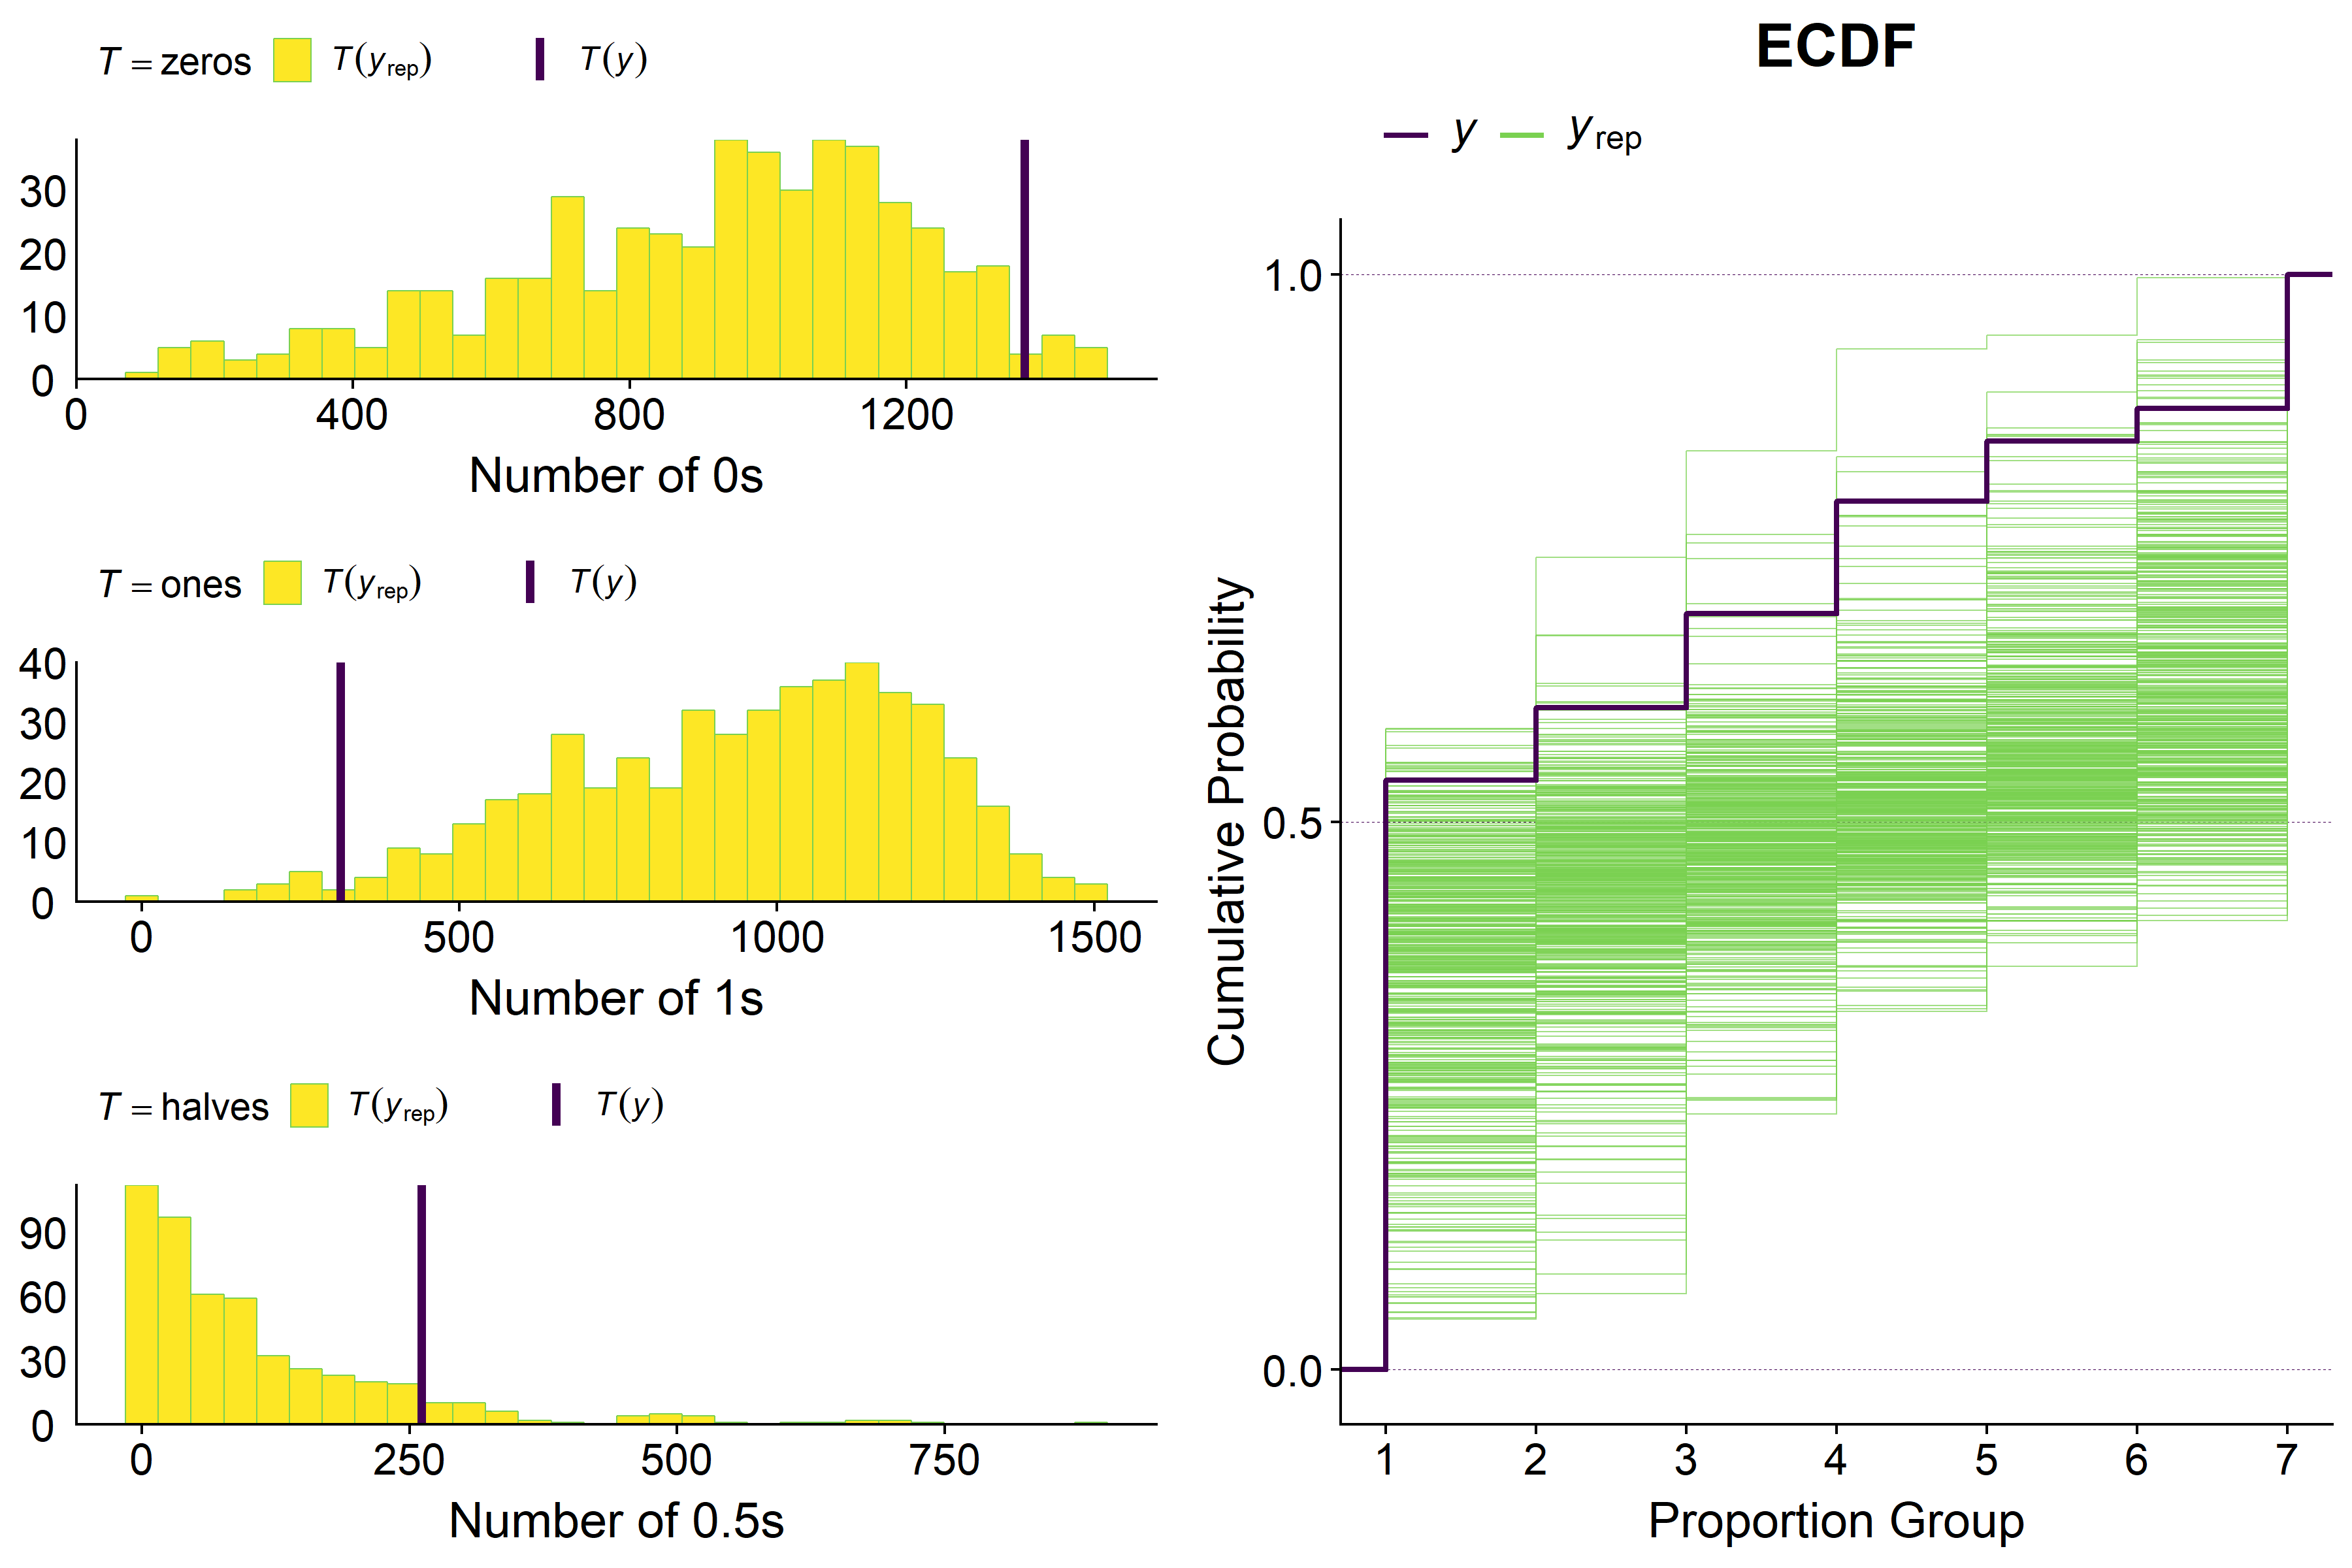
\includegraphics[width=0.85\textwidth]{Figures/3_1_Primary_PriPred.png}
	\caption{Prior Predictive Plots} \label{fig::3_PriorPred}	
\end{figure}

\newpage

\subsection{Model Fit and Algorithm Diagnostics}

We ran 3 chains, with warmup of 2000, and 5000 total iterations per chain, meaning 9000 post warmup samples with combined chains. This may seem small for those familiar with Gibbs sampling, however the NUTS (\citeauthor{Hoffman2014}, \citeyear{Hoffman2014}) allows for convergence with fewer samples, as the effective size per iteration is much higher (\citeauthor{Burknerbrms1}, \citeyear{Burknerbrms1}). \\

The model had 0 divergent transitions\footnote{Divergent transitions are an indicator of potential bias in the HMC algorithm, and are a more sensitive diagnostic than the usual $\hat{R}$ measure. For more information, see the online case study by \cite{BetancourtDivergence2017}.}. The split $\hat{R}$ should be below 1.1 for all parameters (\citeauthor{GelmanBDA2013}, \citeyear{GelmanBDA2013}), and our model is below this threshold as per Figure \ref{fig::3_Convergence}. The minimum effective size ratio is above 0.15, meaning our effective sizes are all above 1000 which is regarded as usually being enough for stable estimates (\citeauthor{BurknerVuorre2018}, \citeyear{BurknerVuorre2018}). Trace plots display no mixing issues. 

\begin{figure}[h!]
	\centering
	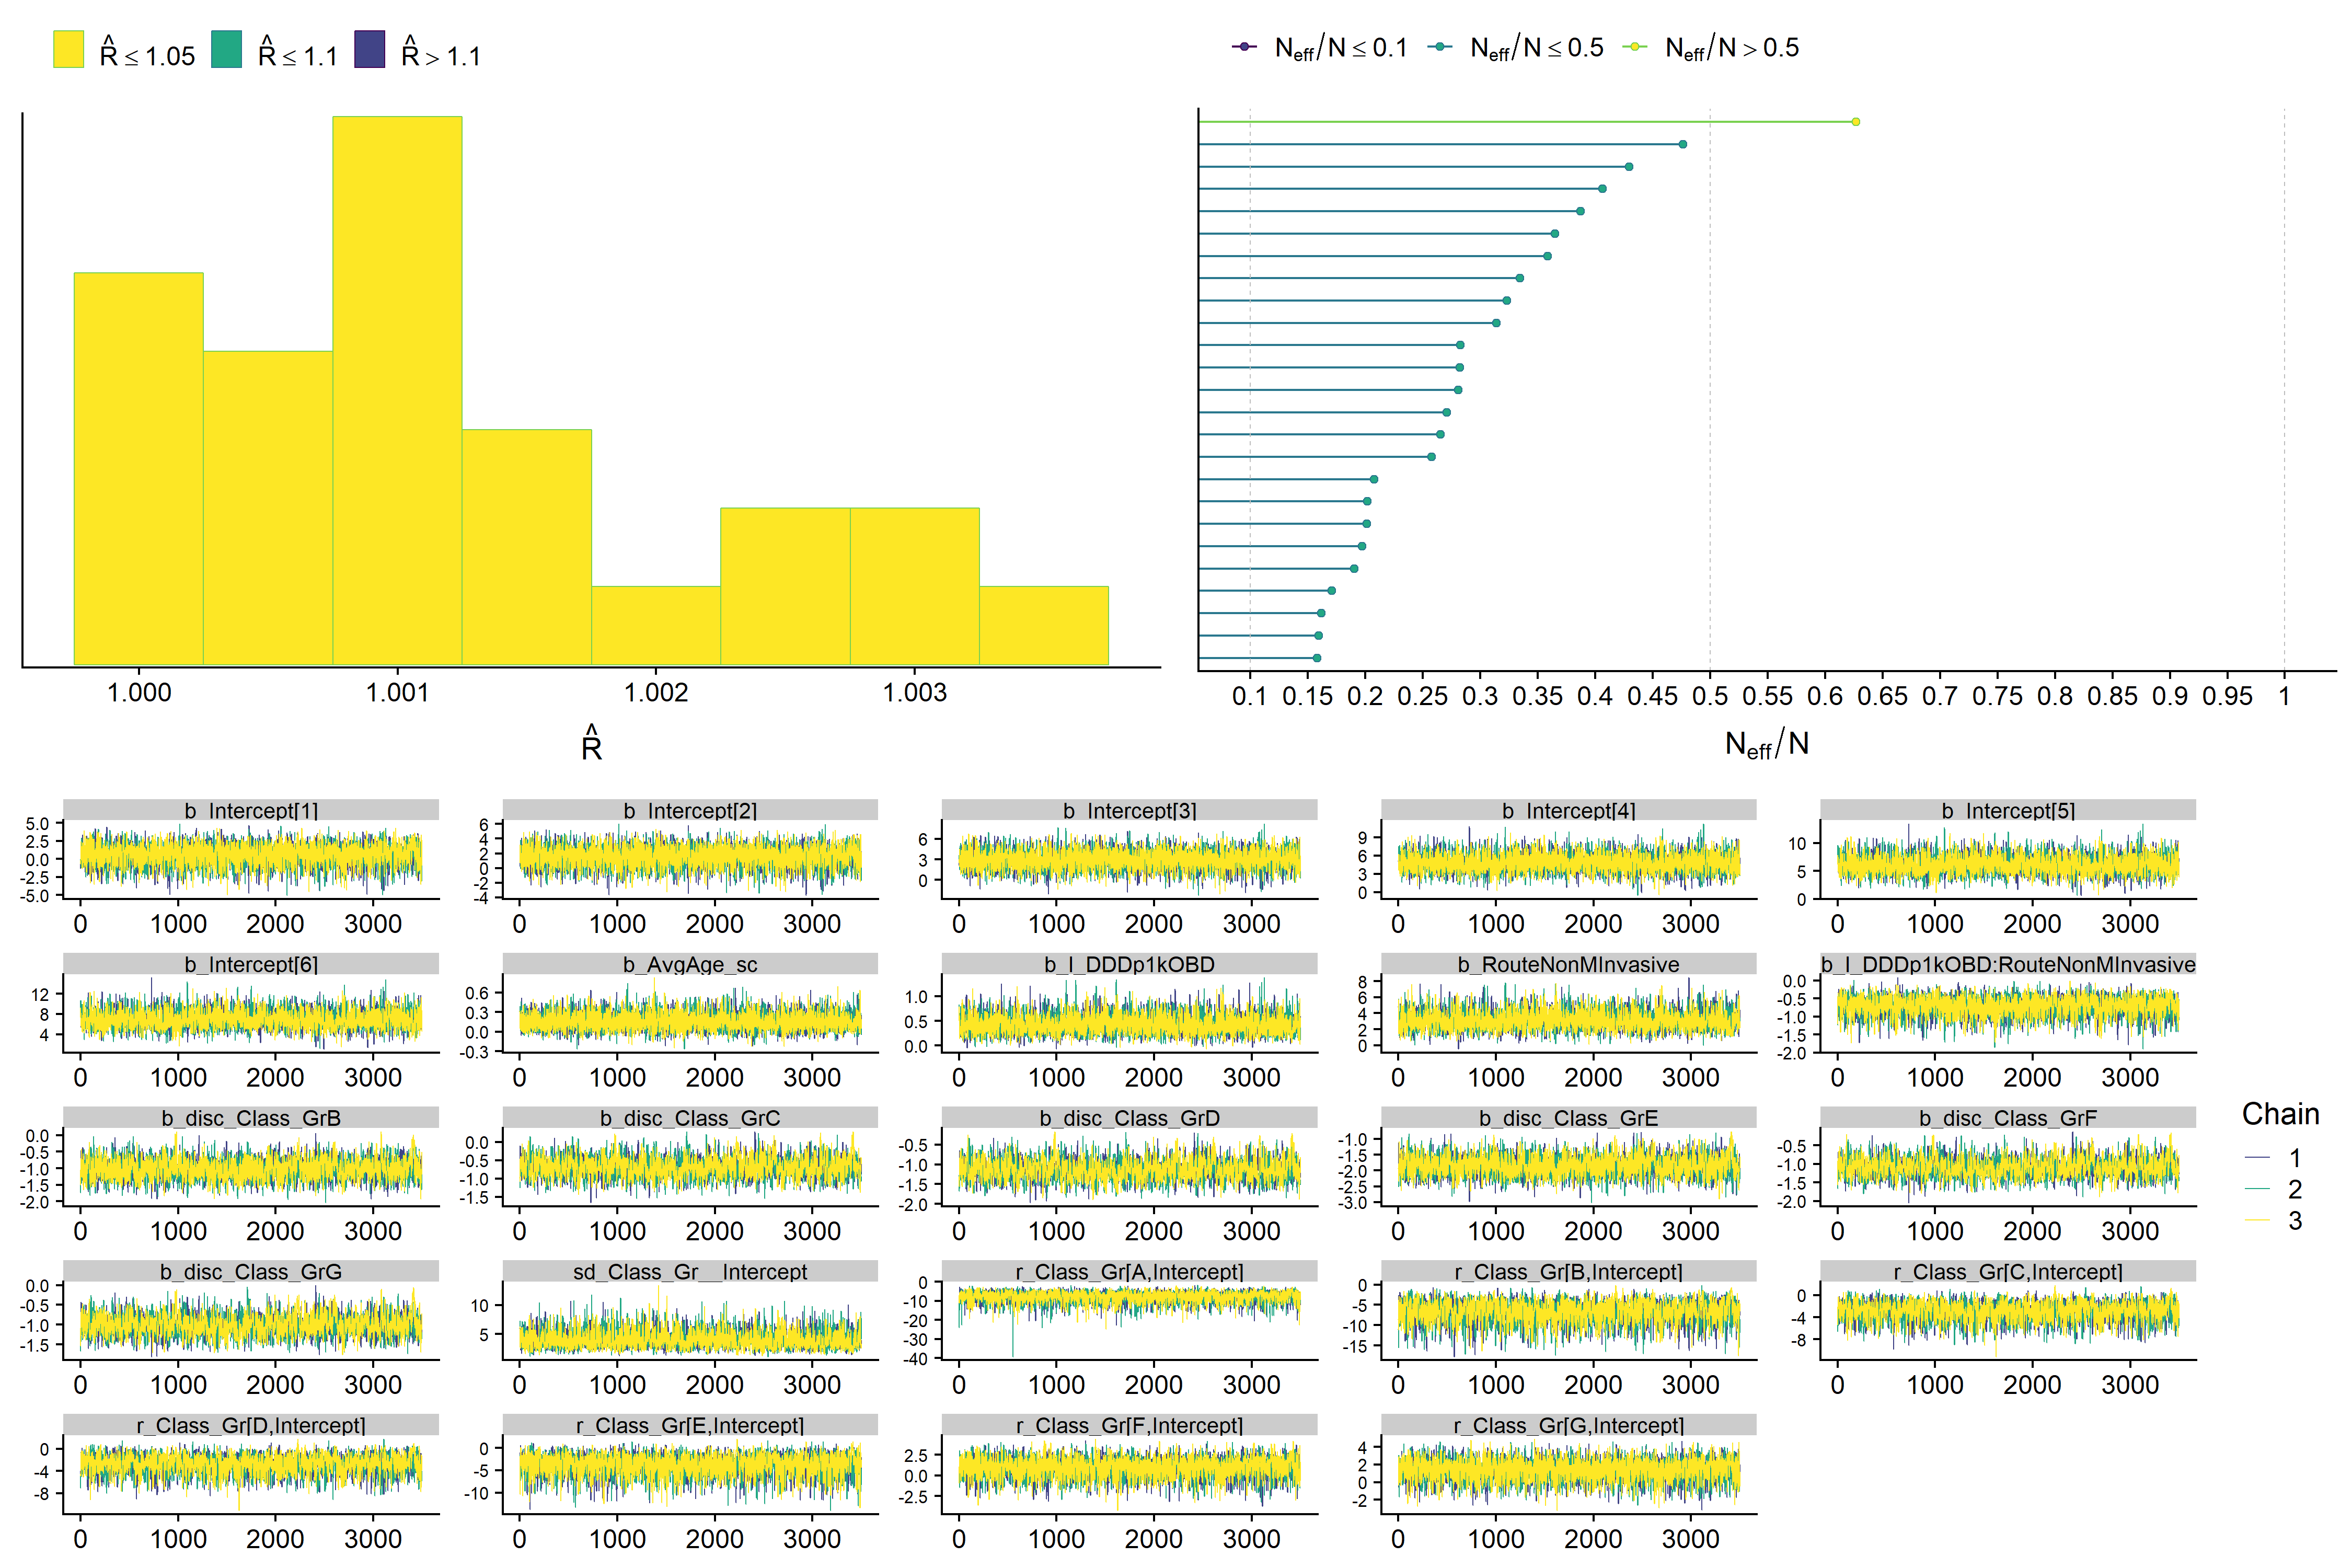
\includegraphics[width = \textwidth, height = 0.5\textheight]{Figures/3_1_Primary_Convergence.png}
	\caption{Convergence Diagnostics and ESS} \label{fig::3_Convergence}	
\end{figure}

\newpage
\subsection{Posterior Predictive (Hypothesis Model)}

This section explores whether the fitted model would be able to generate a dataset similar to what we observed in reality. We do this primarily by computing test statistics, and checking these against the true data. We examine the test statistics split by the class group, to get a more precise look at the data. Posterior predictive checks can be thought of as the Bayesian analogue to goodness-of-fit tests. 

Figure \ref{fig::3_Predictive_BarClass} shows the count of each proportion group segmented by the class group. We see that the counts within each class largely match up to the observed values. The 2nd class in group F however looks suspect, with a relatively low level of uncertainty, yet being above the true count indicated by the bar. There is a substantial amount of variation in groups E to G, suggesting there is a lot of uncertainty around these posterior frequencies. 

\begin{figure}[h!]
	\centering
	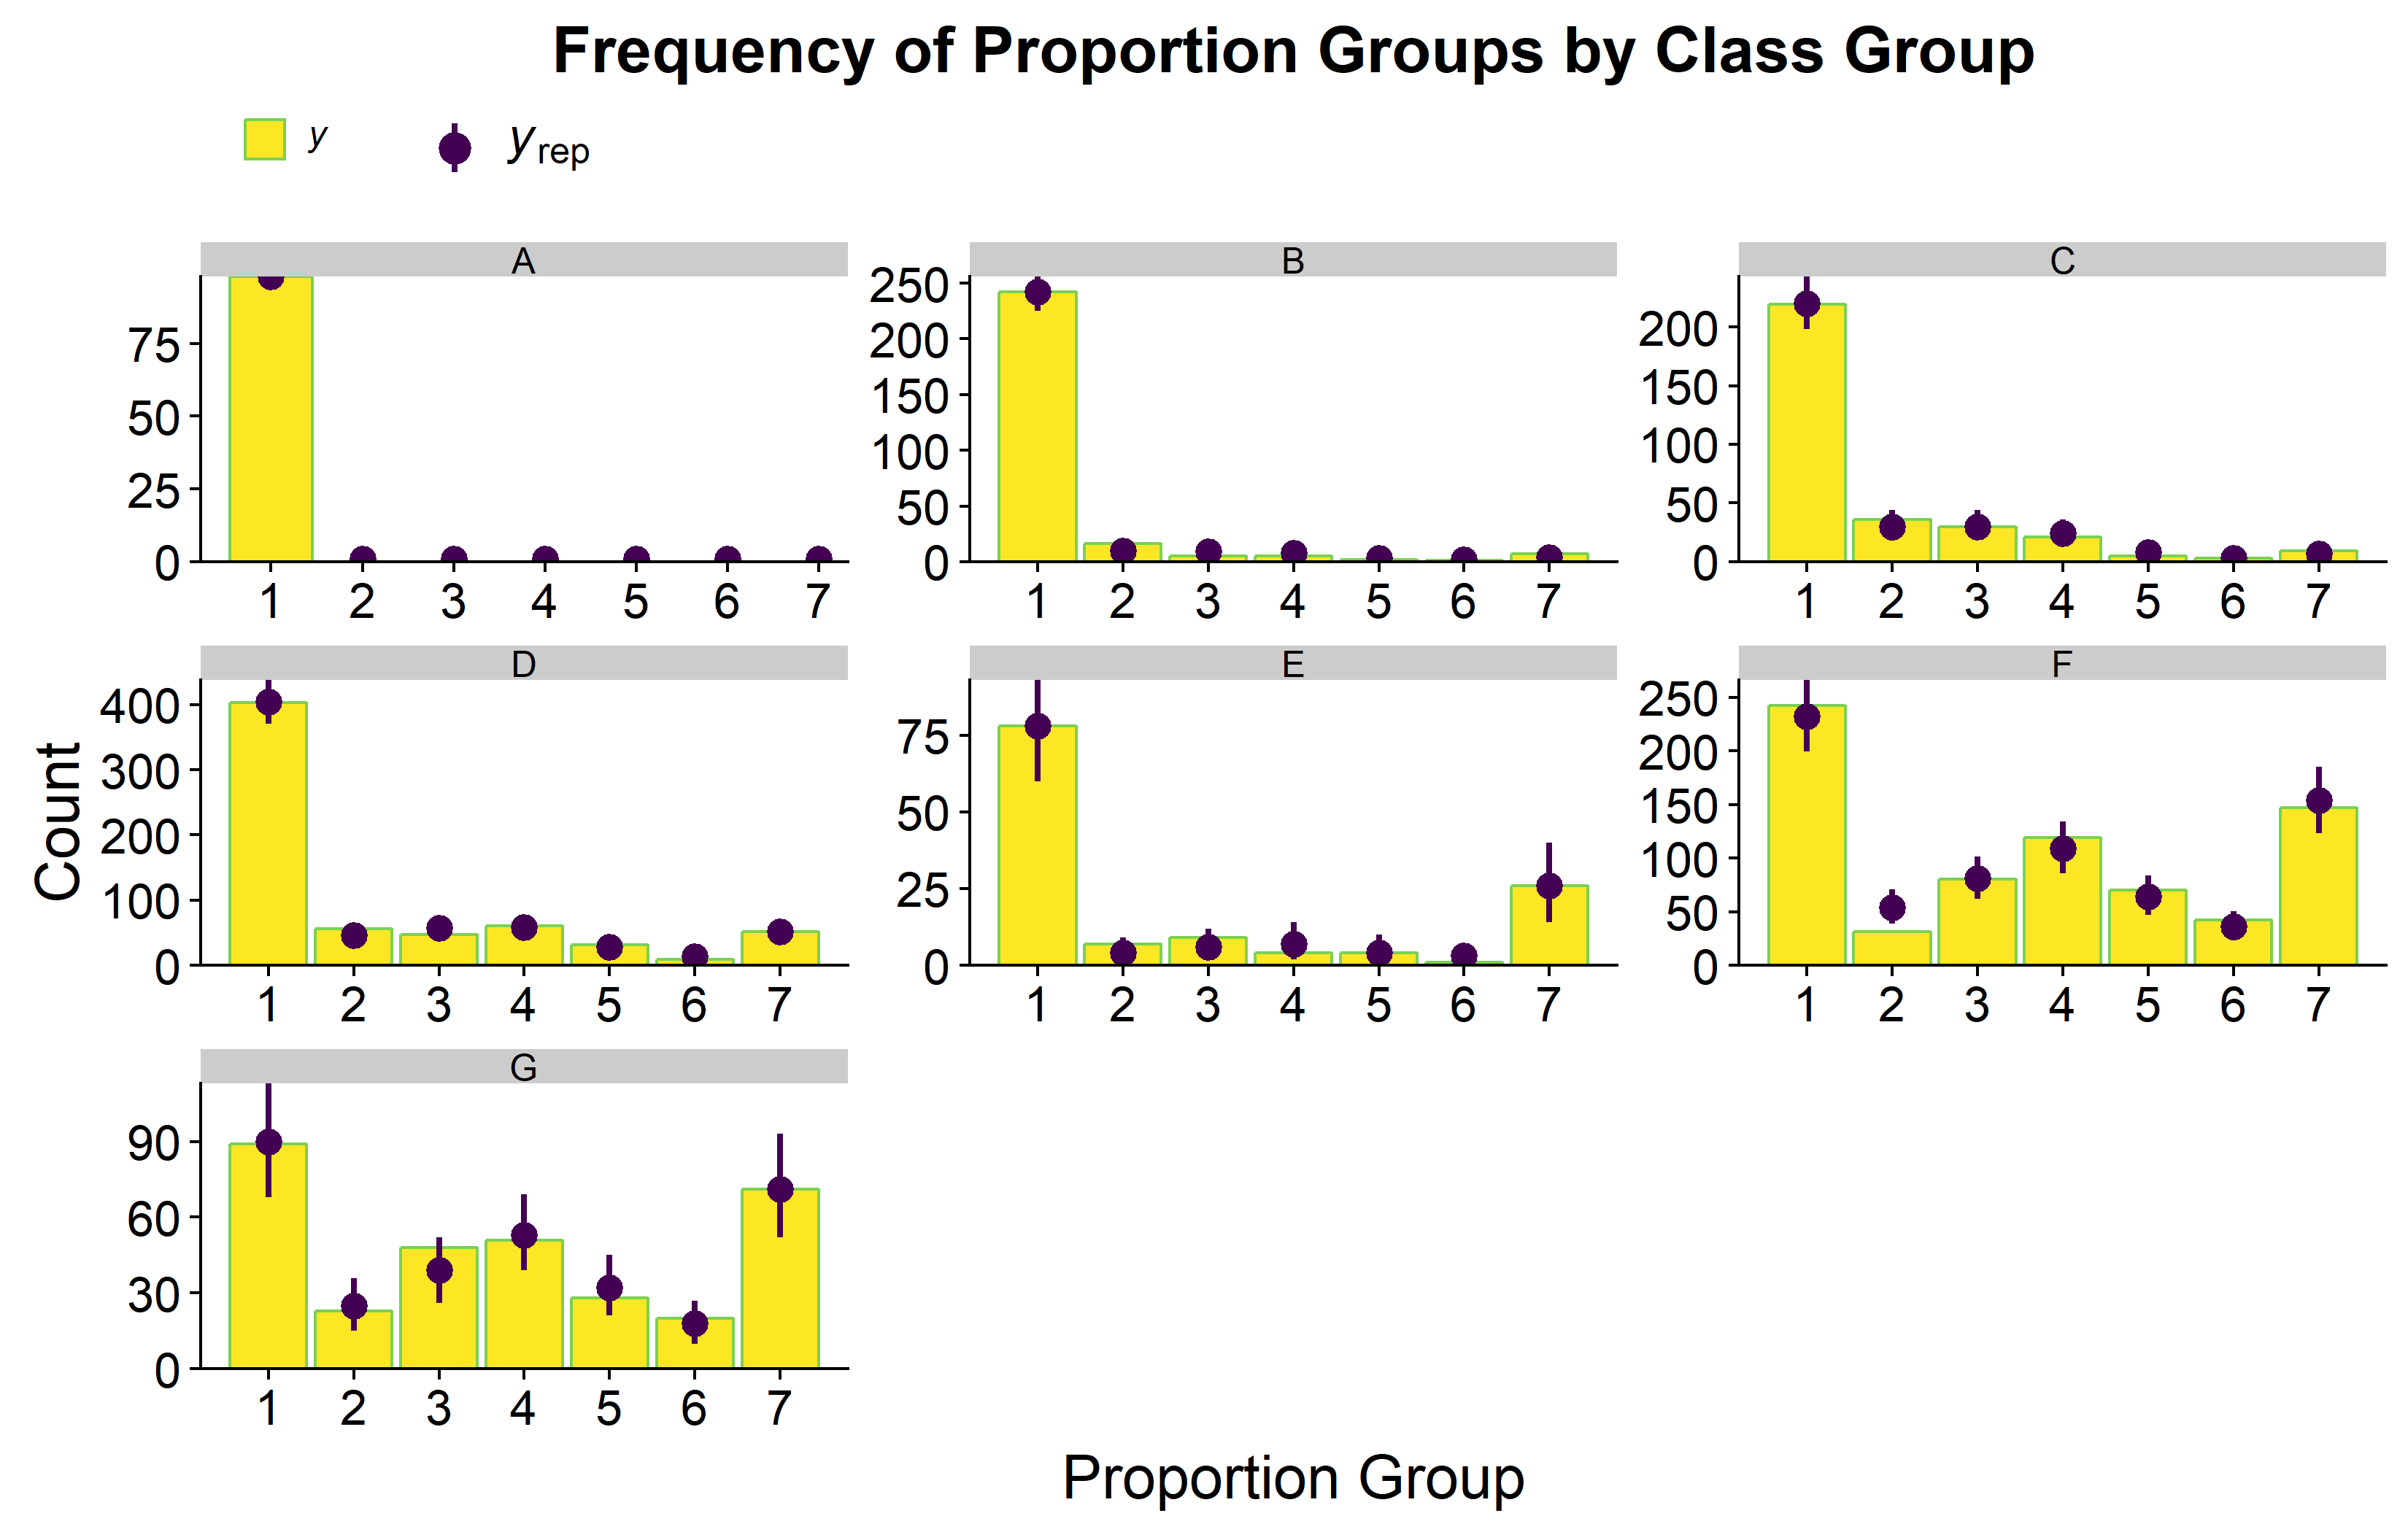
\includegraphics[width =  0.9\textwidth, height = 0.37\textheight]{Figures/3_1_Primary_PostPred_BarClass.png}
	\caption{Frequency Plot by Grouped Class} \label{fig::3_Predictive_BarClass}	
\end{figure}


Figure \ref{fig::3_Predictive_ECDF} shows the density of the overall dataset appears to be well fitted by the simulations from the posterior predictive. 


\begin{figure}[h!]
	\centering
	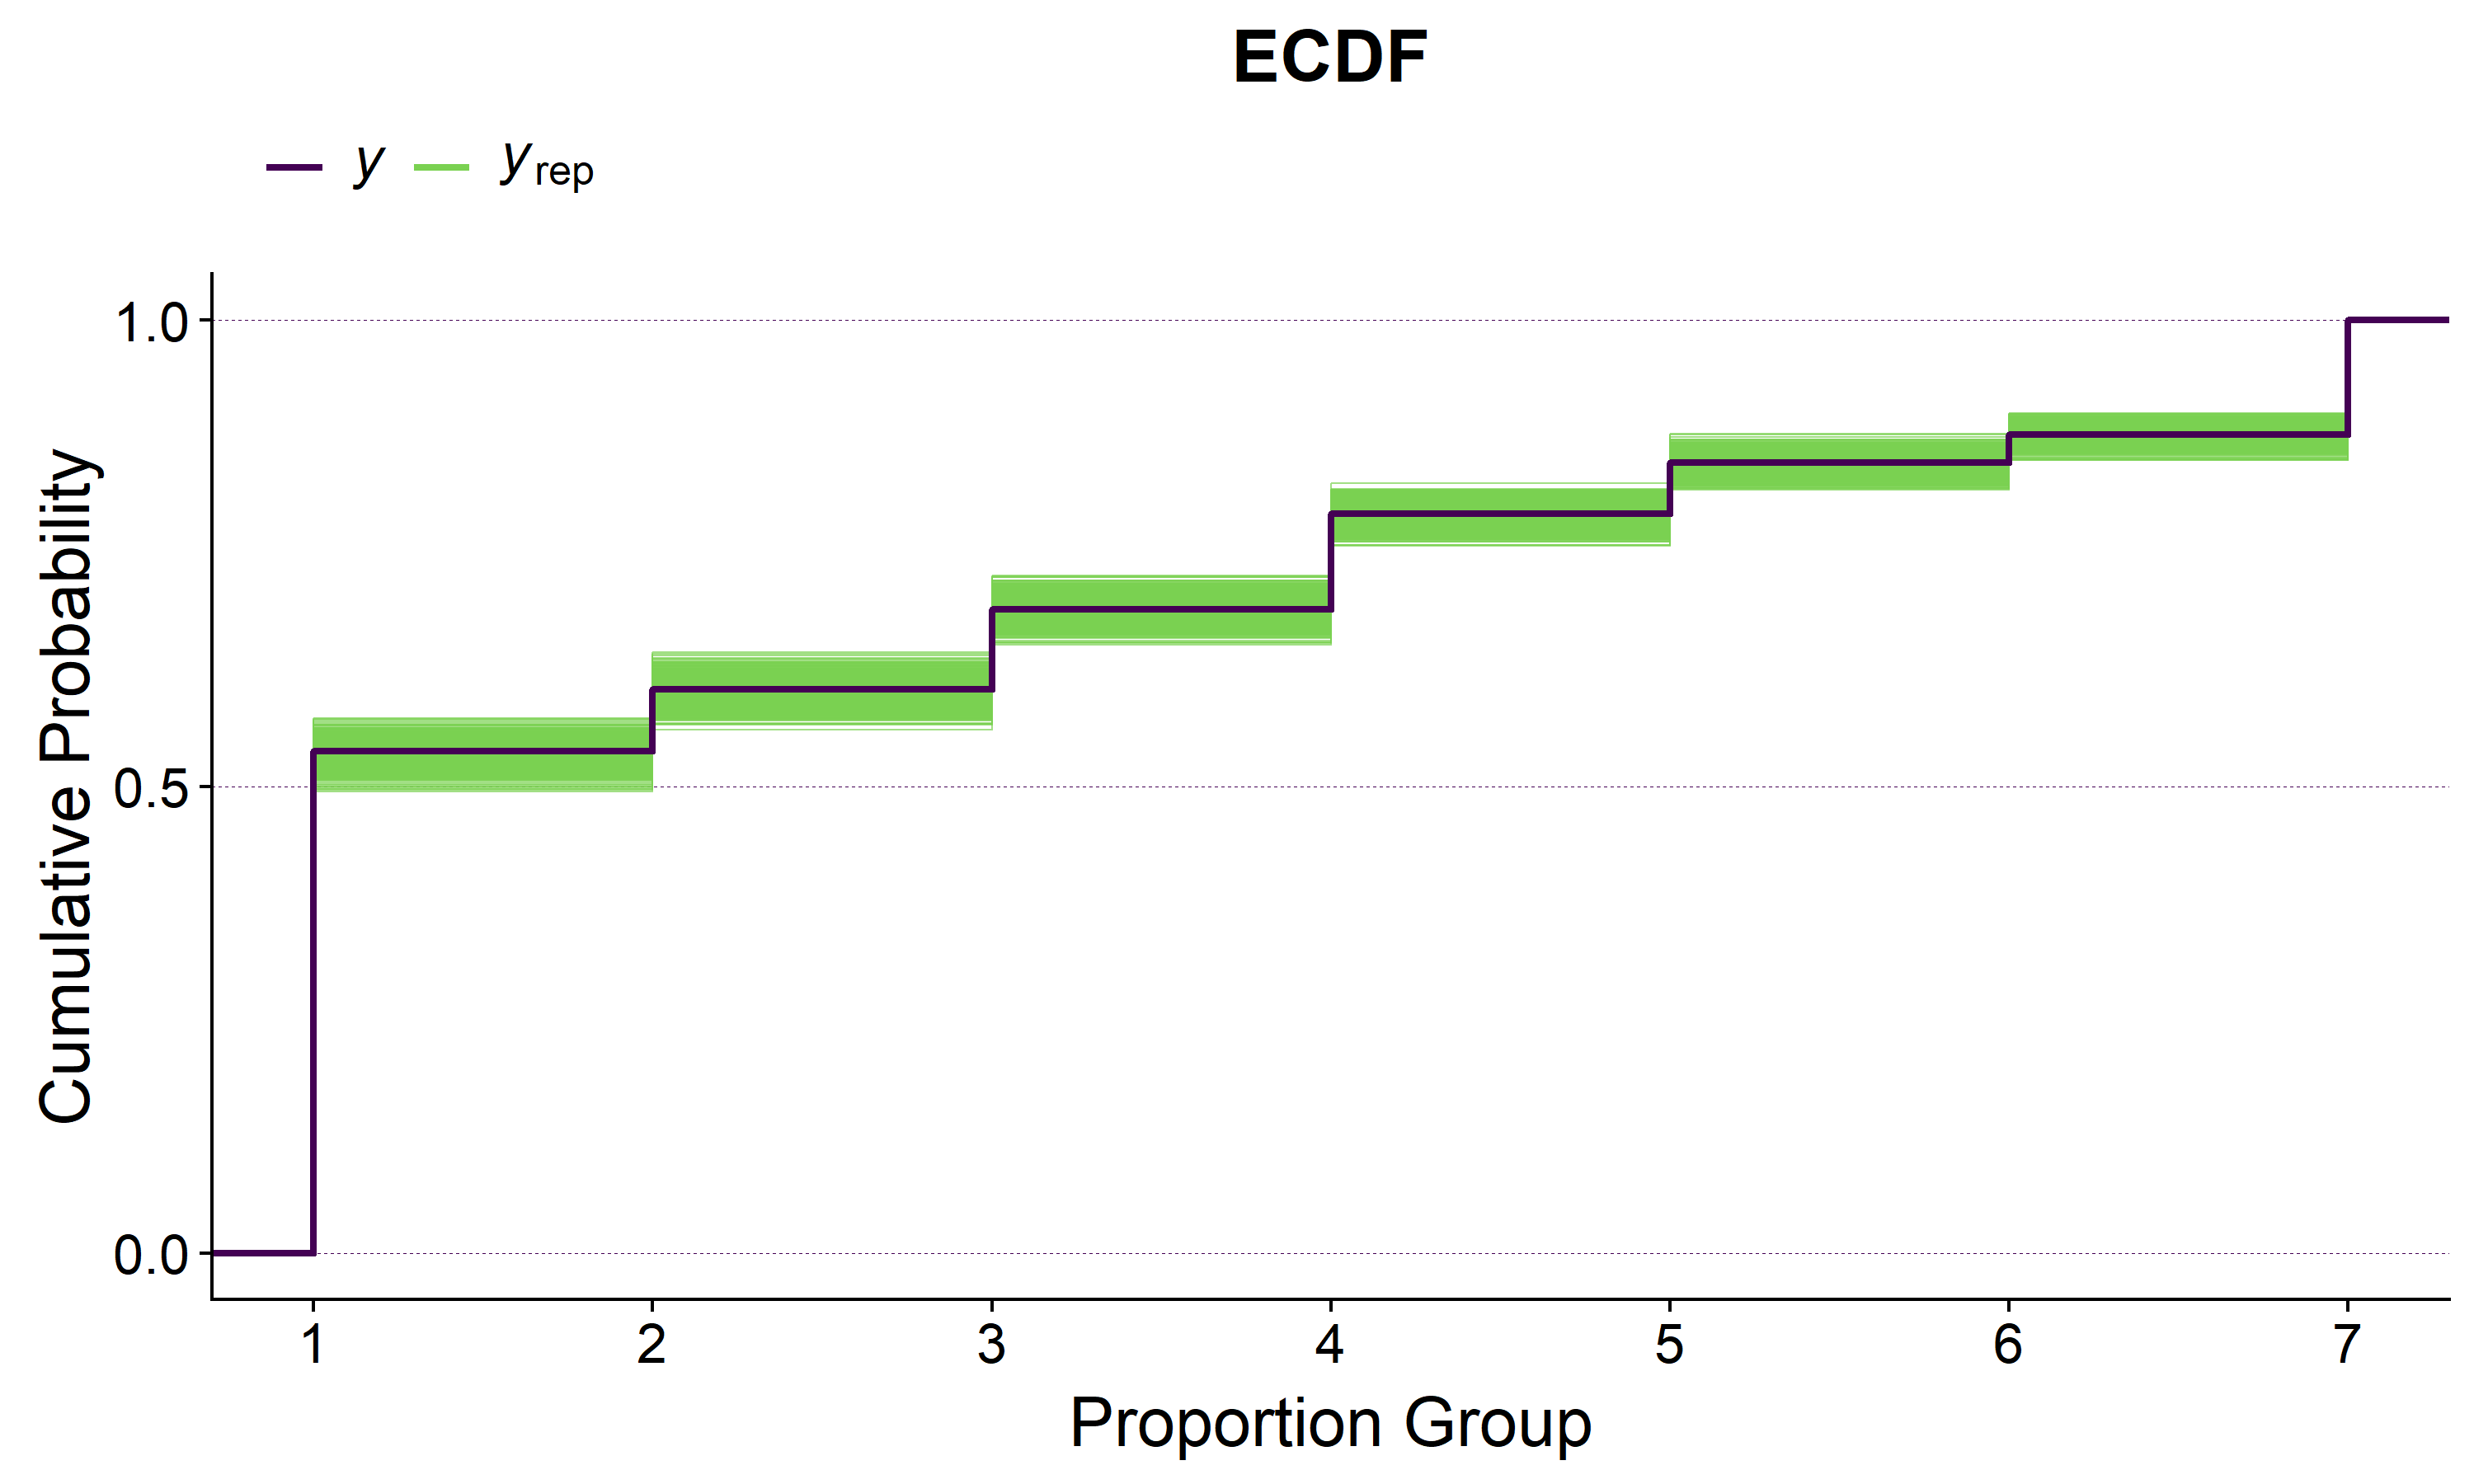
\includegraphics[height = 0.28\textheight]{Figures/3_1_Primary_PostPred_ECDF.png}
	\caption{Posterior ECDF} \label{fig::3_Predictive_ECDF}	
\end{figure}


Figure \ref{fig::3_Predictive_Stats} shows the distribution of the counts of 0s, 0.5s and 1s within each class group. In general, the model captures the test statistics well. However the number of 1s in B is slightly underestimated. The number of 0.5s is not unreasonable for any groups, however B, E, and F are slightly off center. On the whole, these test statistics show an adequate fit to the data. 

\begin{figure}[h!]
	\centering
	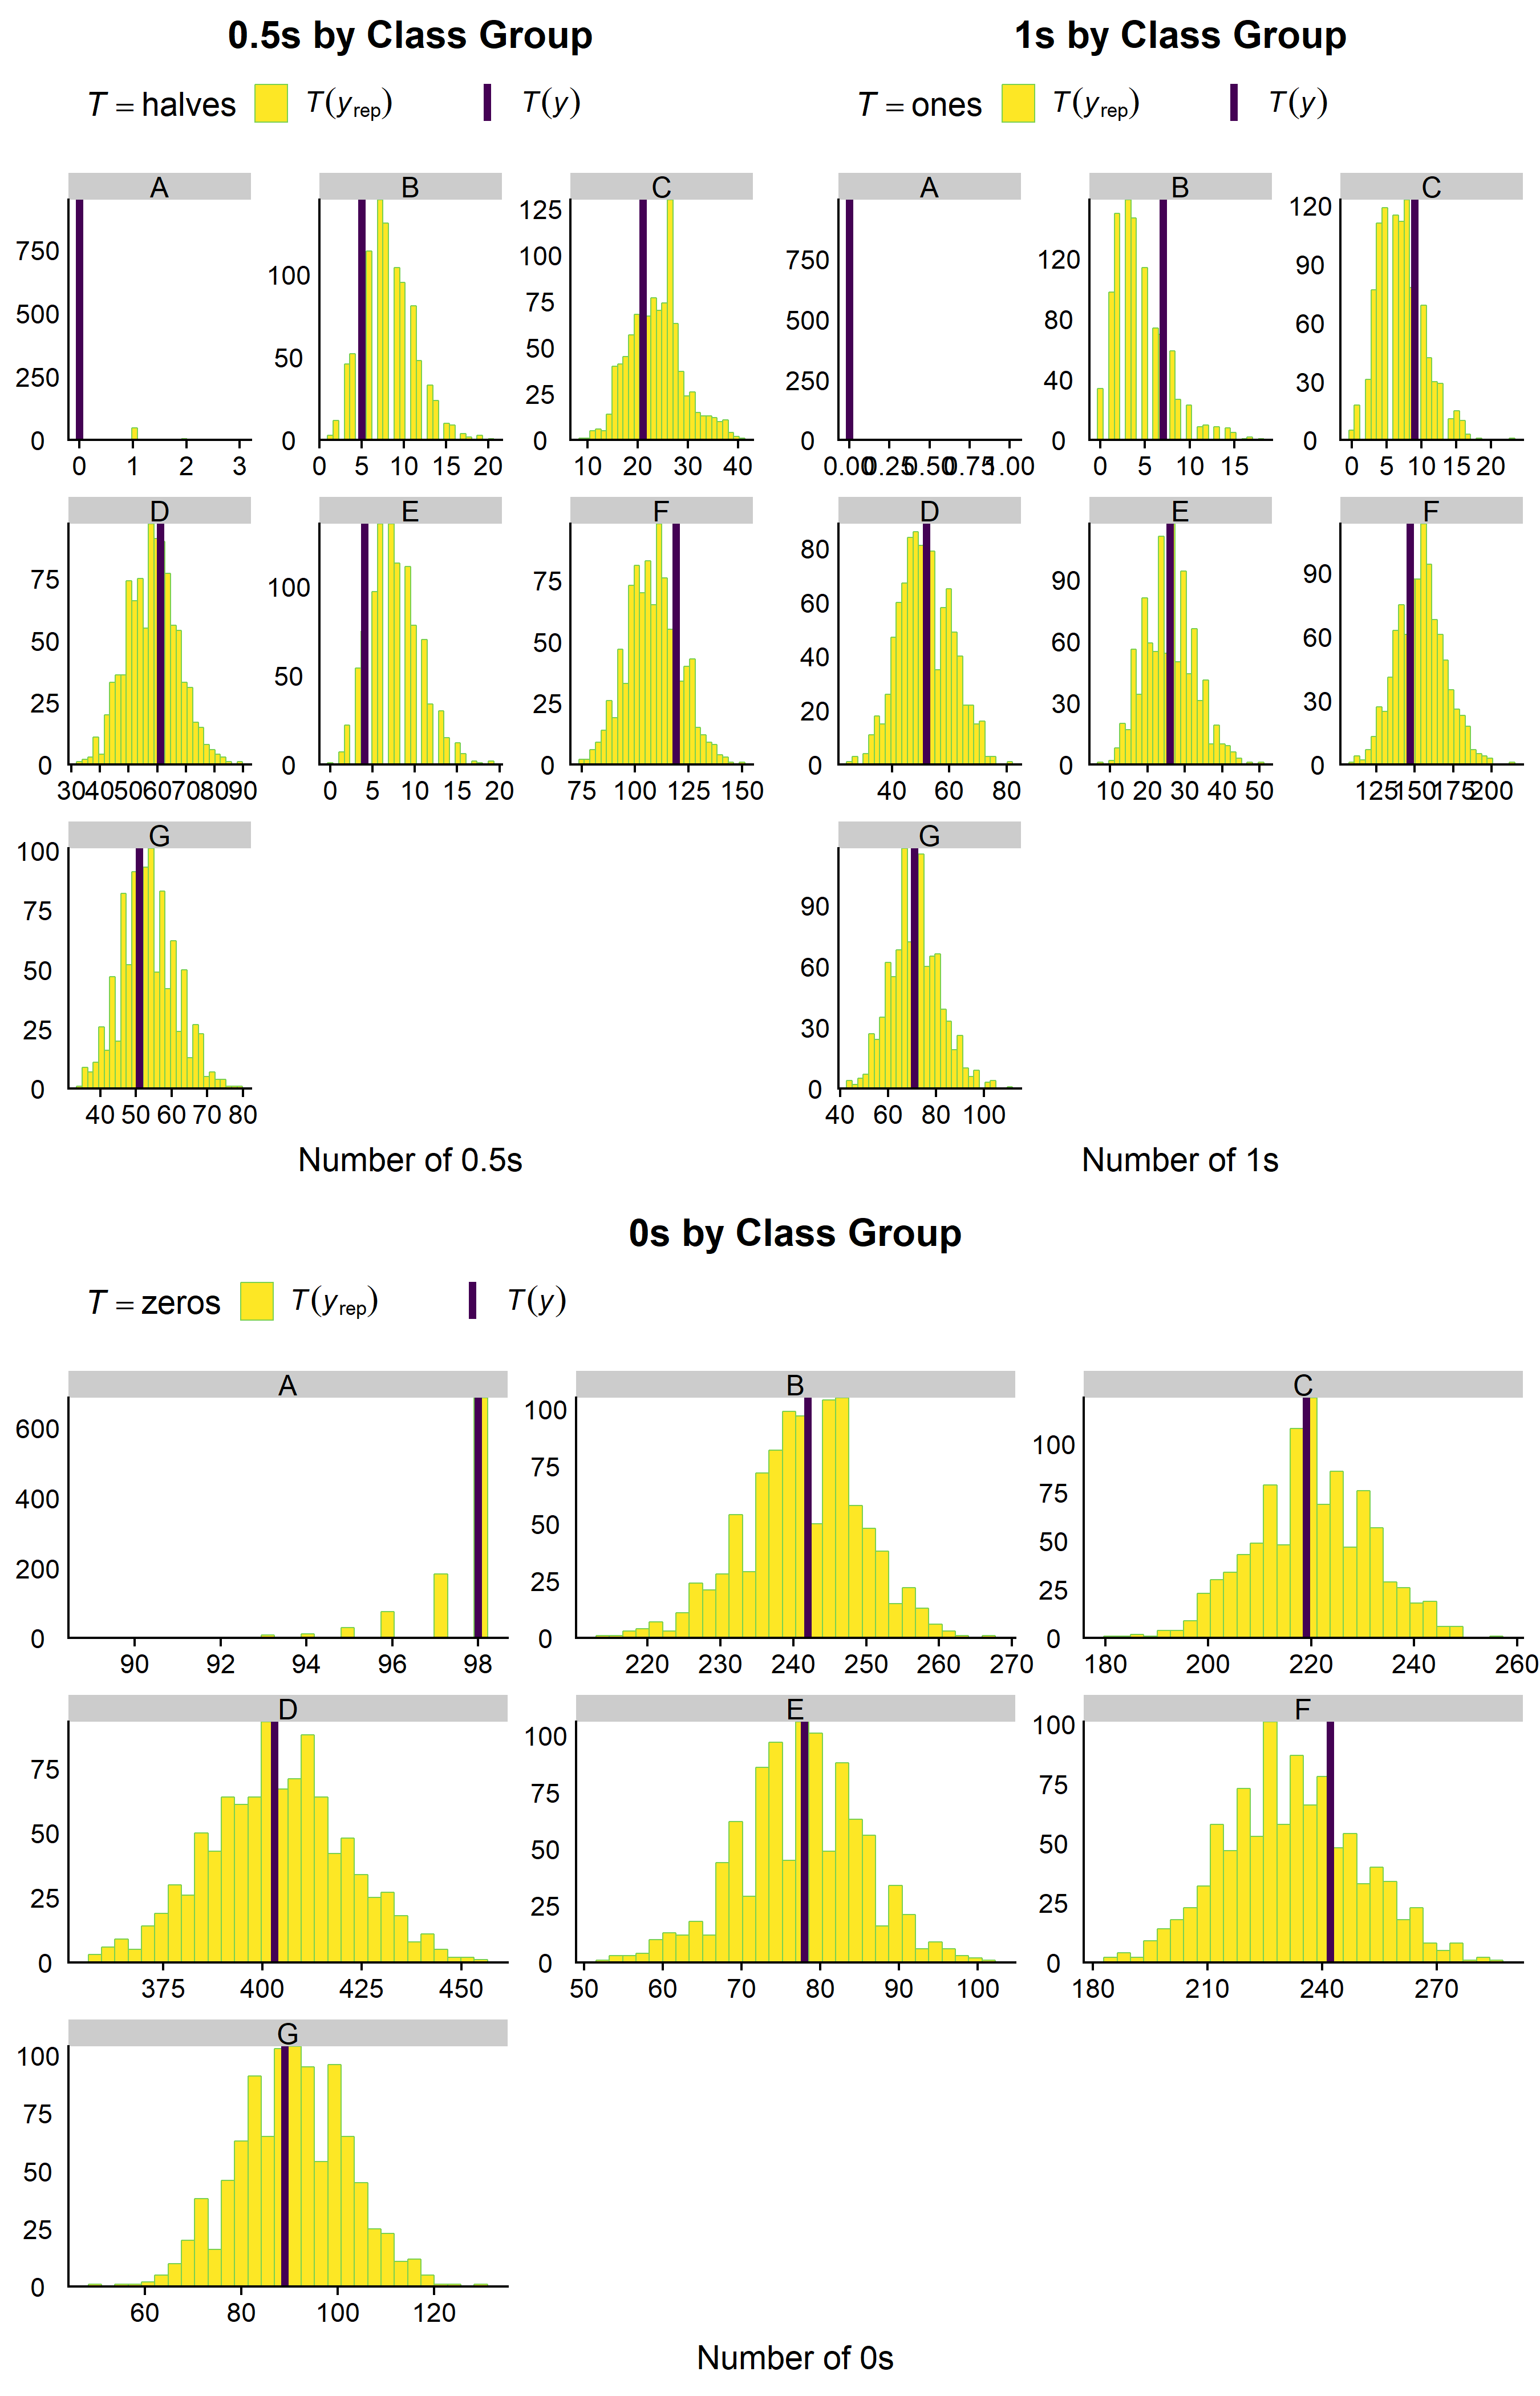
\includegraphics[height = 0.8\textheight]{Figures/3_1_Primary_PostPred_Stats.png}
	\caption{Test Statistics} \label{fig::3_Predictive_Stats}	
\end{figure}

\newpage

Figure \ref{fig::3_Predictive_BarPred} shows a similar frequency plot to Figure \ref{fig::3_Predictive_BarClass}, but now the groups are the true observations. In terms of direct predictions the model does poorly, proposing similar patterns within each bin. That is each bin has a peak at 0 and 1, with a wide normal shape on (0,1). Our goal may be inference, however this lack of predictive ability is concerning as it suggests that the data is too variable to predict, meaning we should be sceptical of our coefficients. 

Examining the predicted linear component (i.e. the values on the latent scale) in Figure \ref{fig::3_Primary_LinPred} we see that, as desired, higher bins have a higher value of the latent variable. This breaks down for the 7th group (proportions of 1), but the general trend is promising. This suggests there is \textit{some} ability to distinguish between proportion groups, but that there is too much variance for specific predictions to be made. 

\begin{figure}[h!]
	\centering
	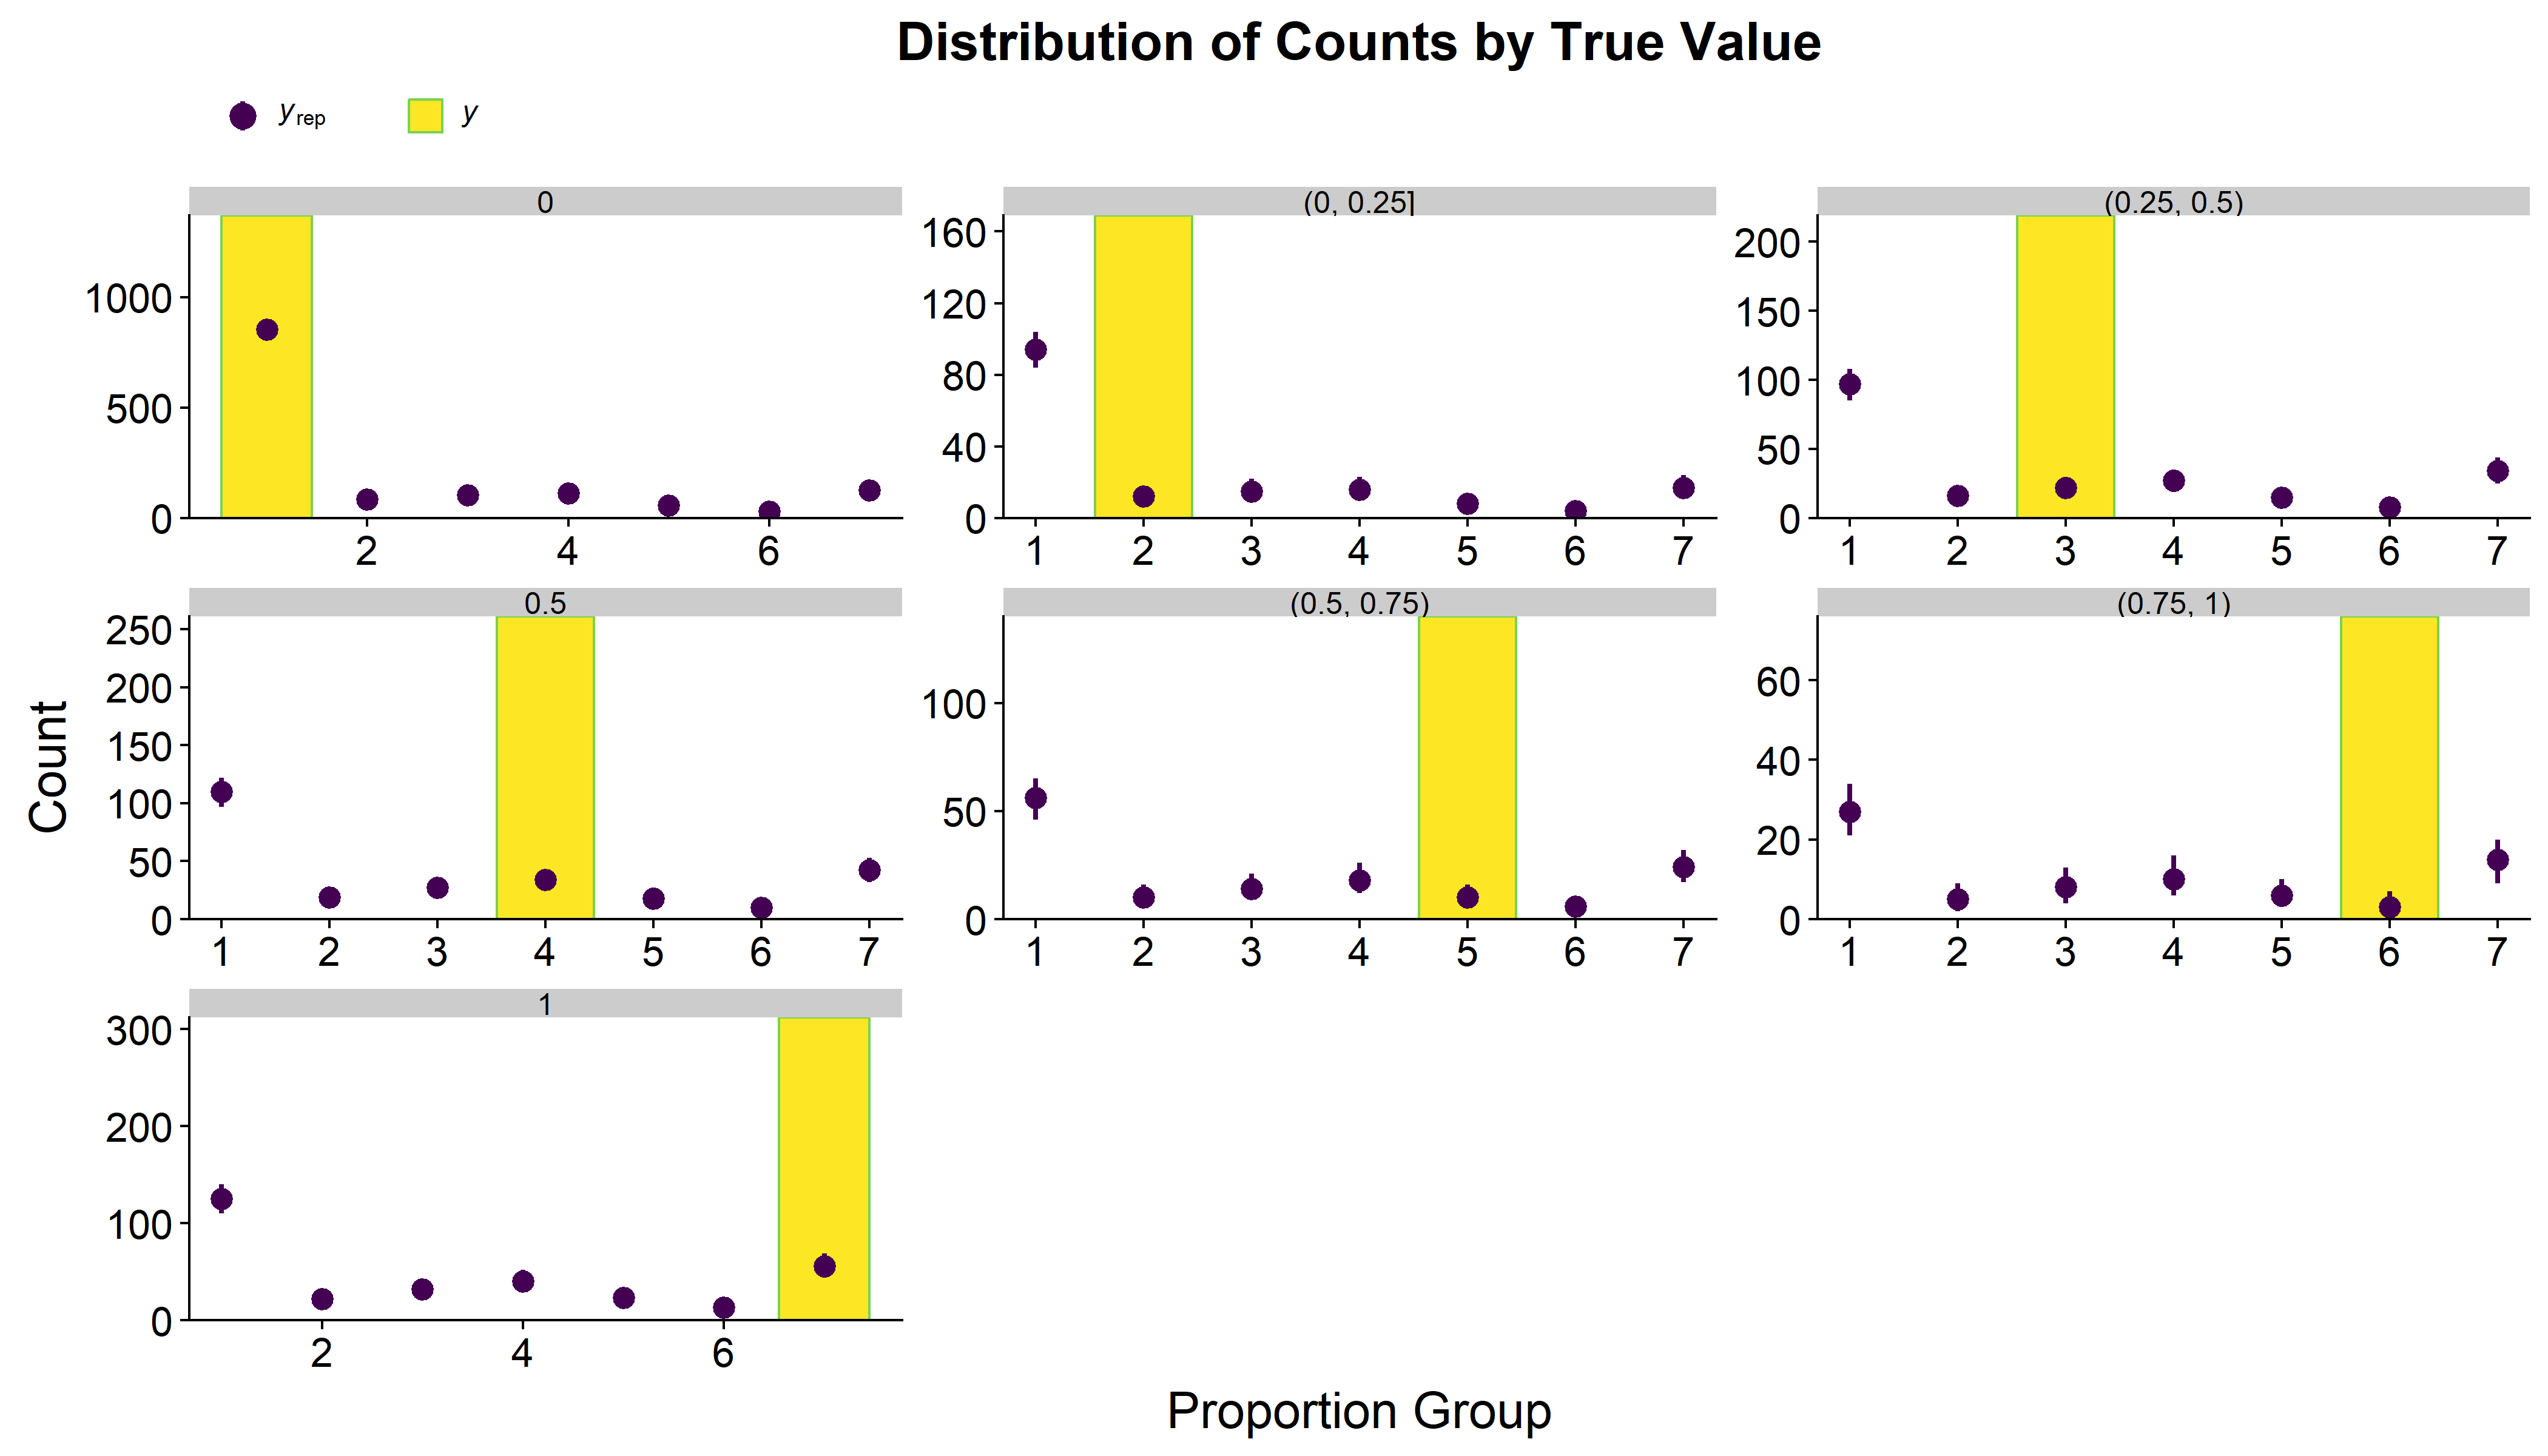
\includegraphics[width = 0.85\textwidth, height = 0.35\textheight]{Figures/3_1_Primary_PostPred_BarPred.png}
	\caption{Frequencies vs True Values} \label{fig::3_Predictive_BarPred}	
\end{figure}

\begin{figure}[h!]
	\centering
	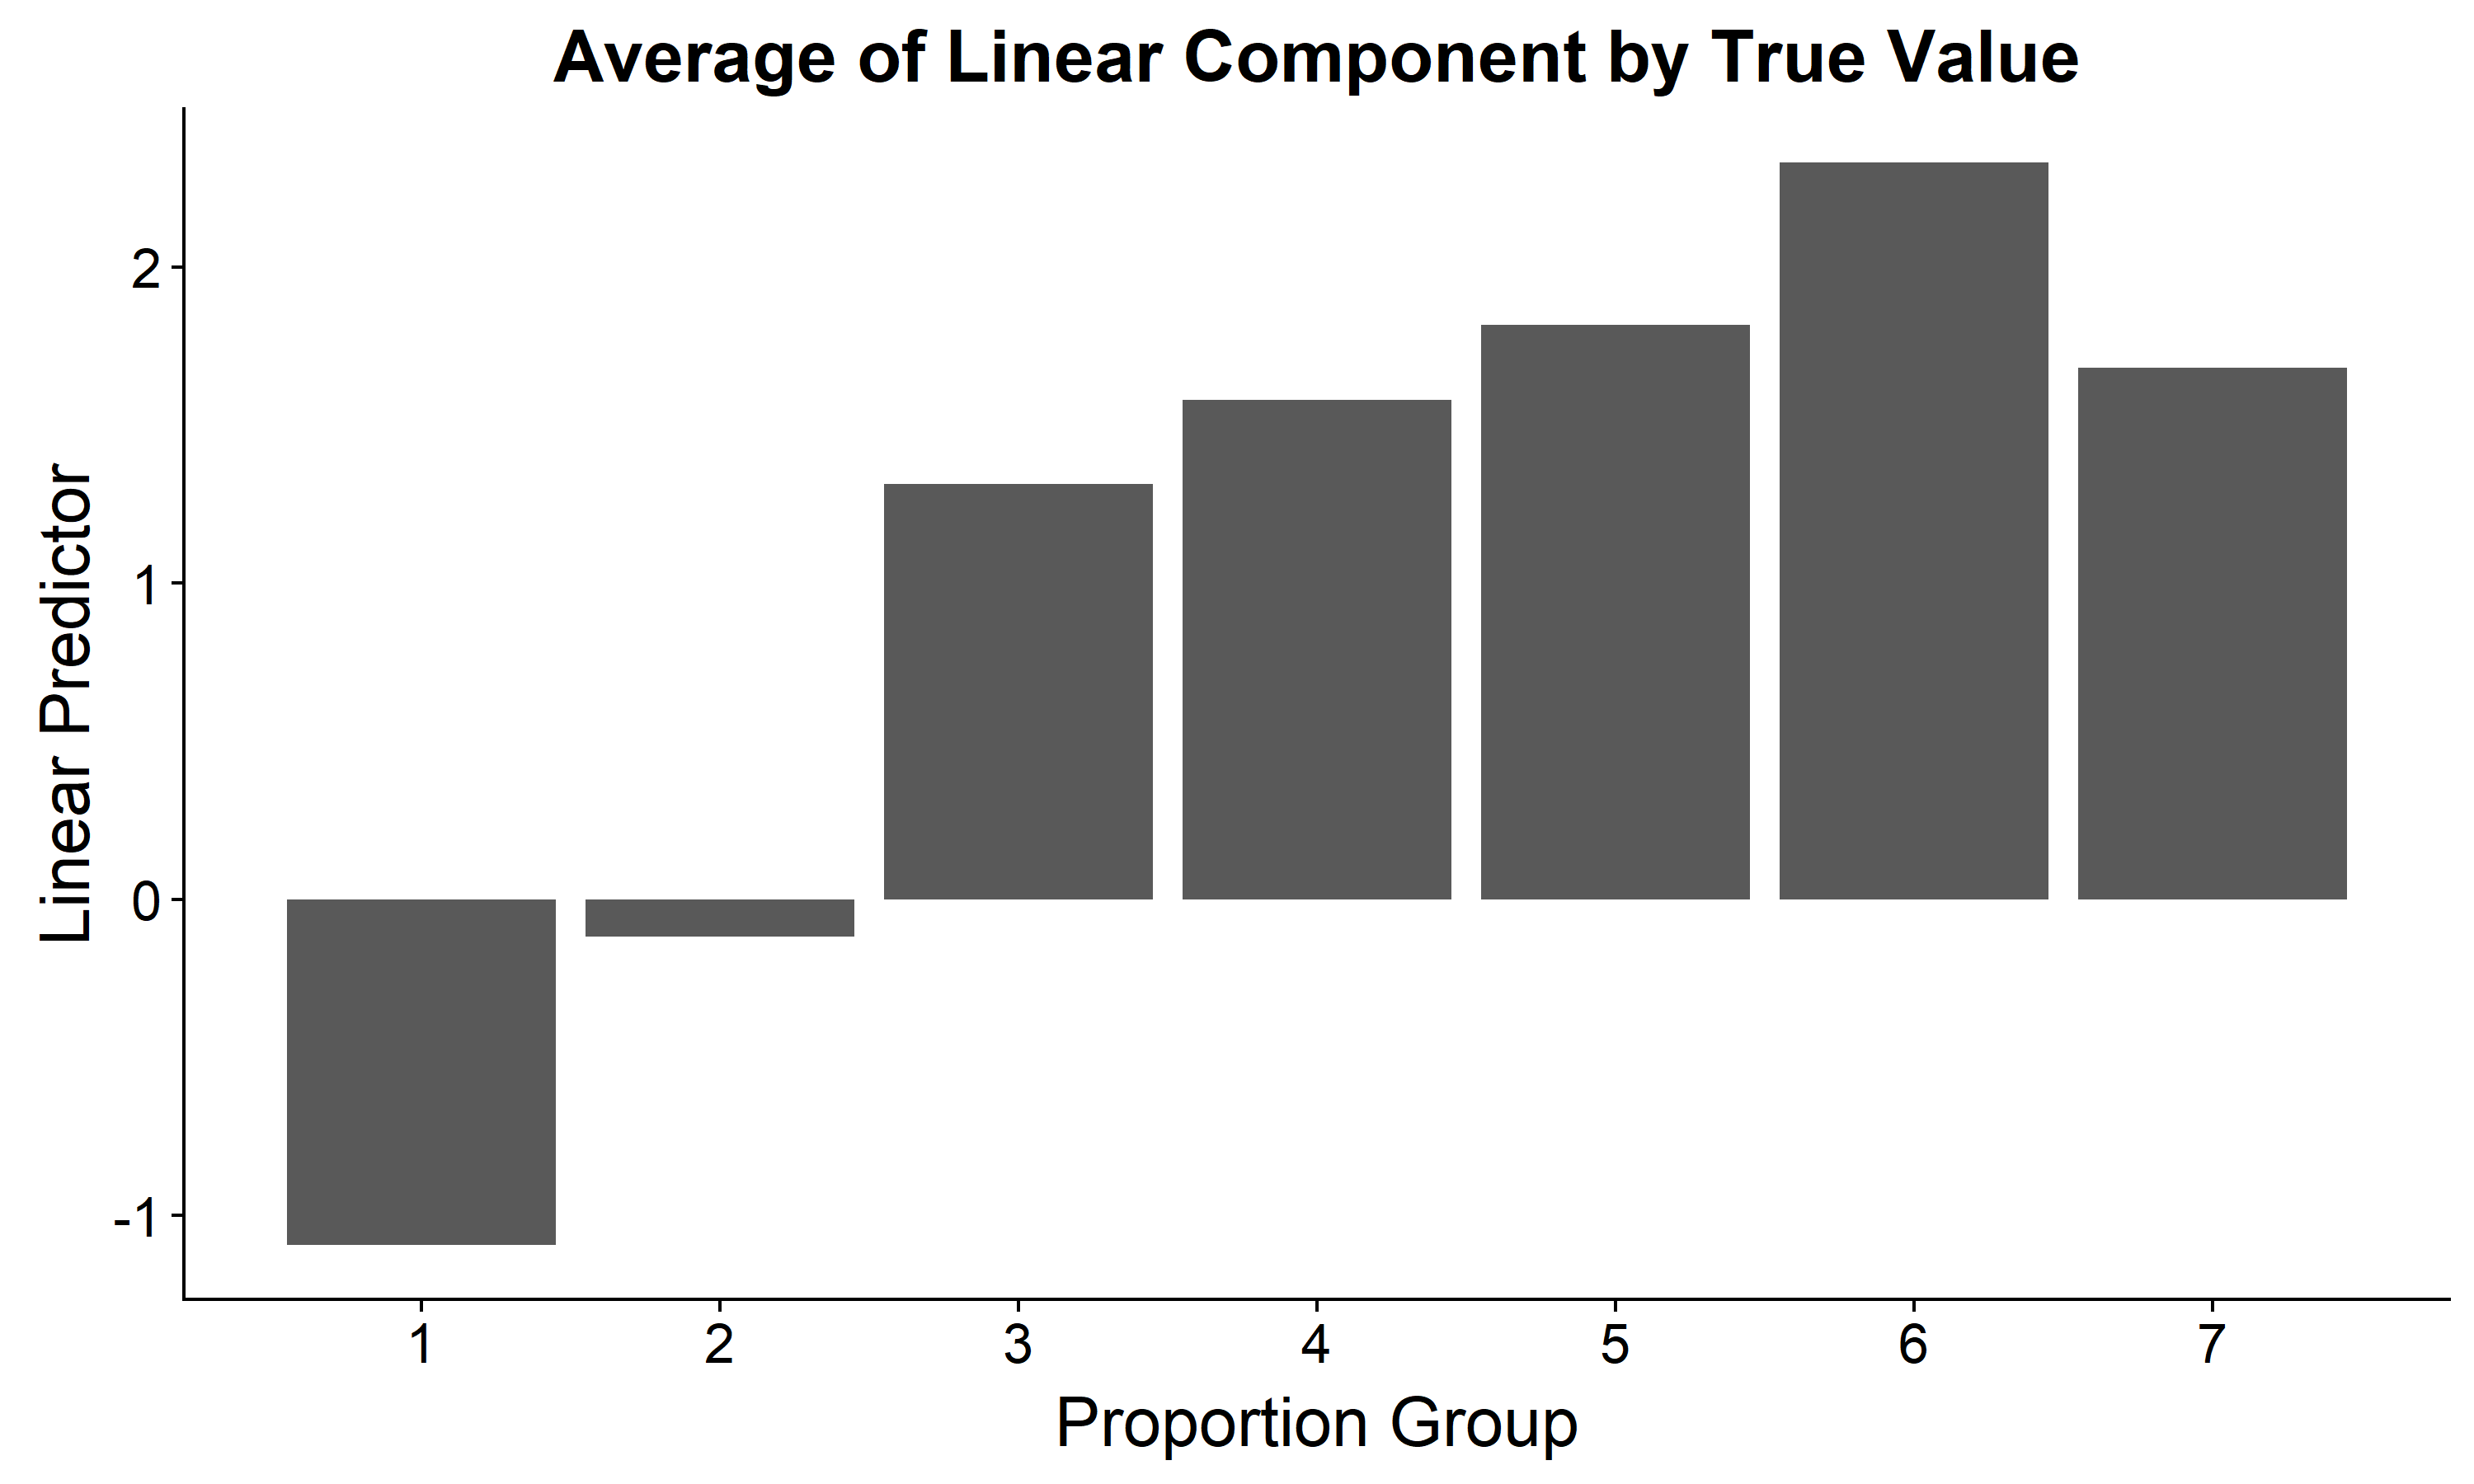
\includegraphics[height = 0.3\textheight]{Figures/3_1_Primary_Linpred.png}
	\caption{Linear Predictor vs. True Group} \label{fig::3_Primary_LinPred}	
\end{figure}





\newpage
\subsection{Model Comparison}

We compare our hypothesised model to alternative formulations to establish room for improvement, using Pareto-smoothed importance sampling leave-one-out cross-validation (PSIS-LOO) (\citeauthor{VehtariPSIS2017}, \citeyear{VehtariPSIS2017}). PSIS-LOO has been established as preferable to the widely applicable information criterion (WAIC) developed by \cite{WatanabeAIC} -- another common model comparison tool. Both aim to approximate the expected log pointwise predictive density (elpd), however WAIC has a larger bias, and the bias-variance tradeoff is harder to control (\citeauthor{VehtariPracEval2017}, \citeyear{VehtariPracEval2017}). In general, we interpret a higher elpd as better, and a model as clearly better if the difference in elpd is greater than 2 standard errors. However this is only a general heuristic, since standard error estimates have high variance (\citeauthor{Piironen2017}, \citeyear{Piironen2017}). 

Details of the models compared are appended. The idea is to use a different group for the group-level effect (drug class, drug name), allow varying slopes, and remove the interaction between DDD and the route. We also use an overfit model to get a rough estimate of the maximum predictive potential on the data under the ordered logit, by plotting the equivalent of Figure \ref{fig::3_Predictive_BarPred} in Figure \ref{fig::3_Overfit_PredPlot}. 

Our hypothesised model is \texttt{mp1}, while comparison models begin with \texttt{mc}. The overfit model is \texttt{mc1}, varying slopes is \texttt{mc2}, \texttt{mc3x} models  use the ungrouped class as the varying intercept, and \texttt{mc4x} models use the drug name. 

No divergent transitions were reported, $\hat{R}$ was below 1.1 for all models, effective sample sizes were all above 1000, and $\hat{k}$ values (a diagnostic for PSIS-LOO) were all less than 0.7 except the overfit model, which had 6 ``bad" values (in (0.7, 1]) and 1 ``very bad" value (above 1). 


\begin{table}[ht]
	\centering
	\begin{tabular}{lllllllll}
		\hline
		Model & elpd\_diff & se\_diff & elpd\_loo & se\_elpd\_loo & p\_loo & se\_p\_loo & looic & se\_looic \\ 
		\hline \hline
		mc41 & 0.00 & 0.00 & -3438.12 & 51.90 & 38.24 & 1.75 & 6876.24 & 103.80 \\ 
		mc43 & -0.64 & 1.71 & -3438.76 & 51.92 & 37.79 & 1.72 & 6877.51 & 103.84 \\ 
		mc44 & -0.89 & 1.64 & -3439.01 & 51.93 & 37.33 & 1.74 & 6878.02 & 103.86 \\ 
		mc42 & -1.23 & 1.89 & -3439.34 & 51.92 & 39.16 & 1.76 & 6878.69 & 103.85 \\ 
		mc1 & -9.90 & 5.08 & -3448.02 & 52.11 & 59.48 & 3.81 & 6896.05 & 104.22 \\ 
		mp1 & -23.73 & 9.80 & -3461.85 & 50.91 & 20.36 & 0.68 & 6923.69 & 101.82 \\ 
		mc2 & -29.85 & 10.30 & -3467.97 & 50.94 & 22.37 & 0.70 & 6935.93 & 101.87 \\ 
		mc31 & -30.03 & 9.45 & -3468.15 & 51.02 & 27.24 & 0.91 & 6936.31 & 102.04 \\ 
		mc34 & -36.42 & 10.07 & -3474.54 & 51.03 & 26.27 & 0.88 & 6949.08 & 102.06 \\ 
		mc33 & -36.70 & 10.15 & -3474.82 & 51.01 & 26.25 & 0.88 & 6949.64 & 102.02 \\ 
		mc32 & -37.17 & 9.98 & -3475.29 & 51.03 & 28.94 & 0.92 & 6950.58 & 102.06 \\ 
		\hline
	\end{tabular}
	\caption{Model Comparison} 
	\label{table::4_Model_Comp}
\end{table}



Table \ref{table::4_Model_Comp} implies a varying intercept for the class group is poor relative to a name-varying intercept, but better than the raw class. In general, population-level effects for the age with an interaction between the route and DDD performed better than alternatives. This can be seen as \texttt{mc41} and \texttt{mc31} are better than others within their group, and \texttt{mp1} is better than \texttt{mc2}. The overfit model performs better than our hypothesised model, however this elpd approximation is likely very biased due to the high $\hat{k}$ values. 

The prediction barplot for the overfit model can be seen in Figure \ref{fig::3_Overfit_PredPlot}. Again, the raw predictions themselves do poorly, suggesting there is too much variance in the dataset to generate good predictions. Similarly, Figure \ref{fig::3_Overfit_LinPredPlot} has the same pattern as previously.  

Given the similarity of the ``best" model (\texttt{mc41}) to our hypothesis (the only difference is the group-level intercept), we briefly review the posterior predictive for \texttt{mc41}, and proceed to results.


\begin{figure}[h!]
	\centering
	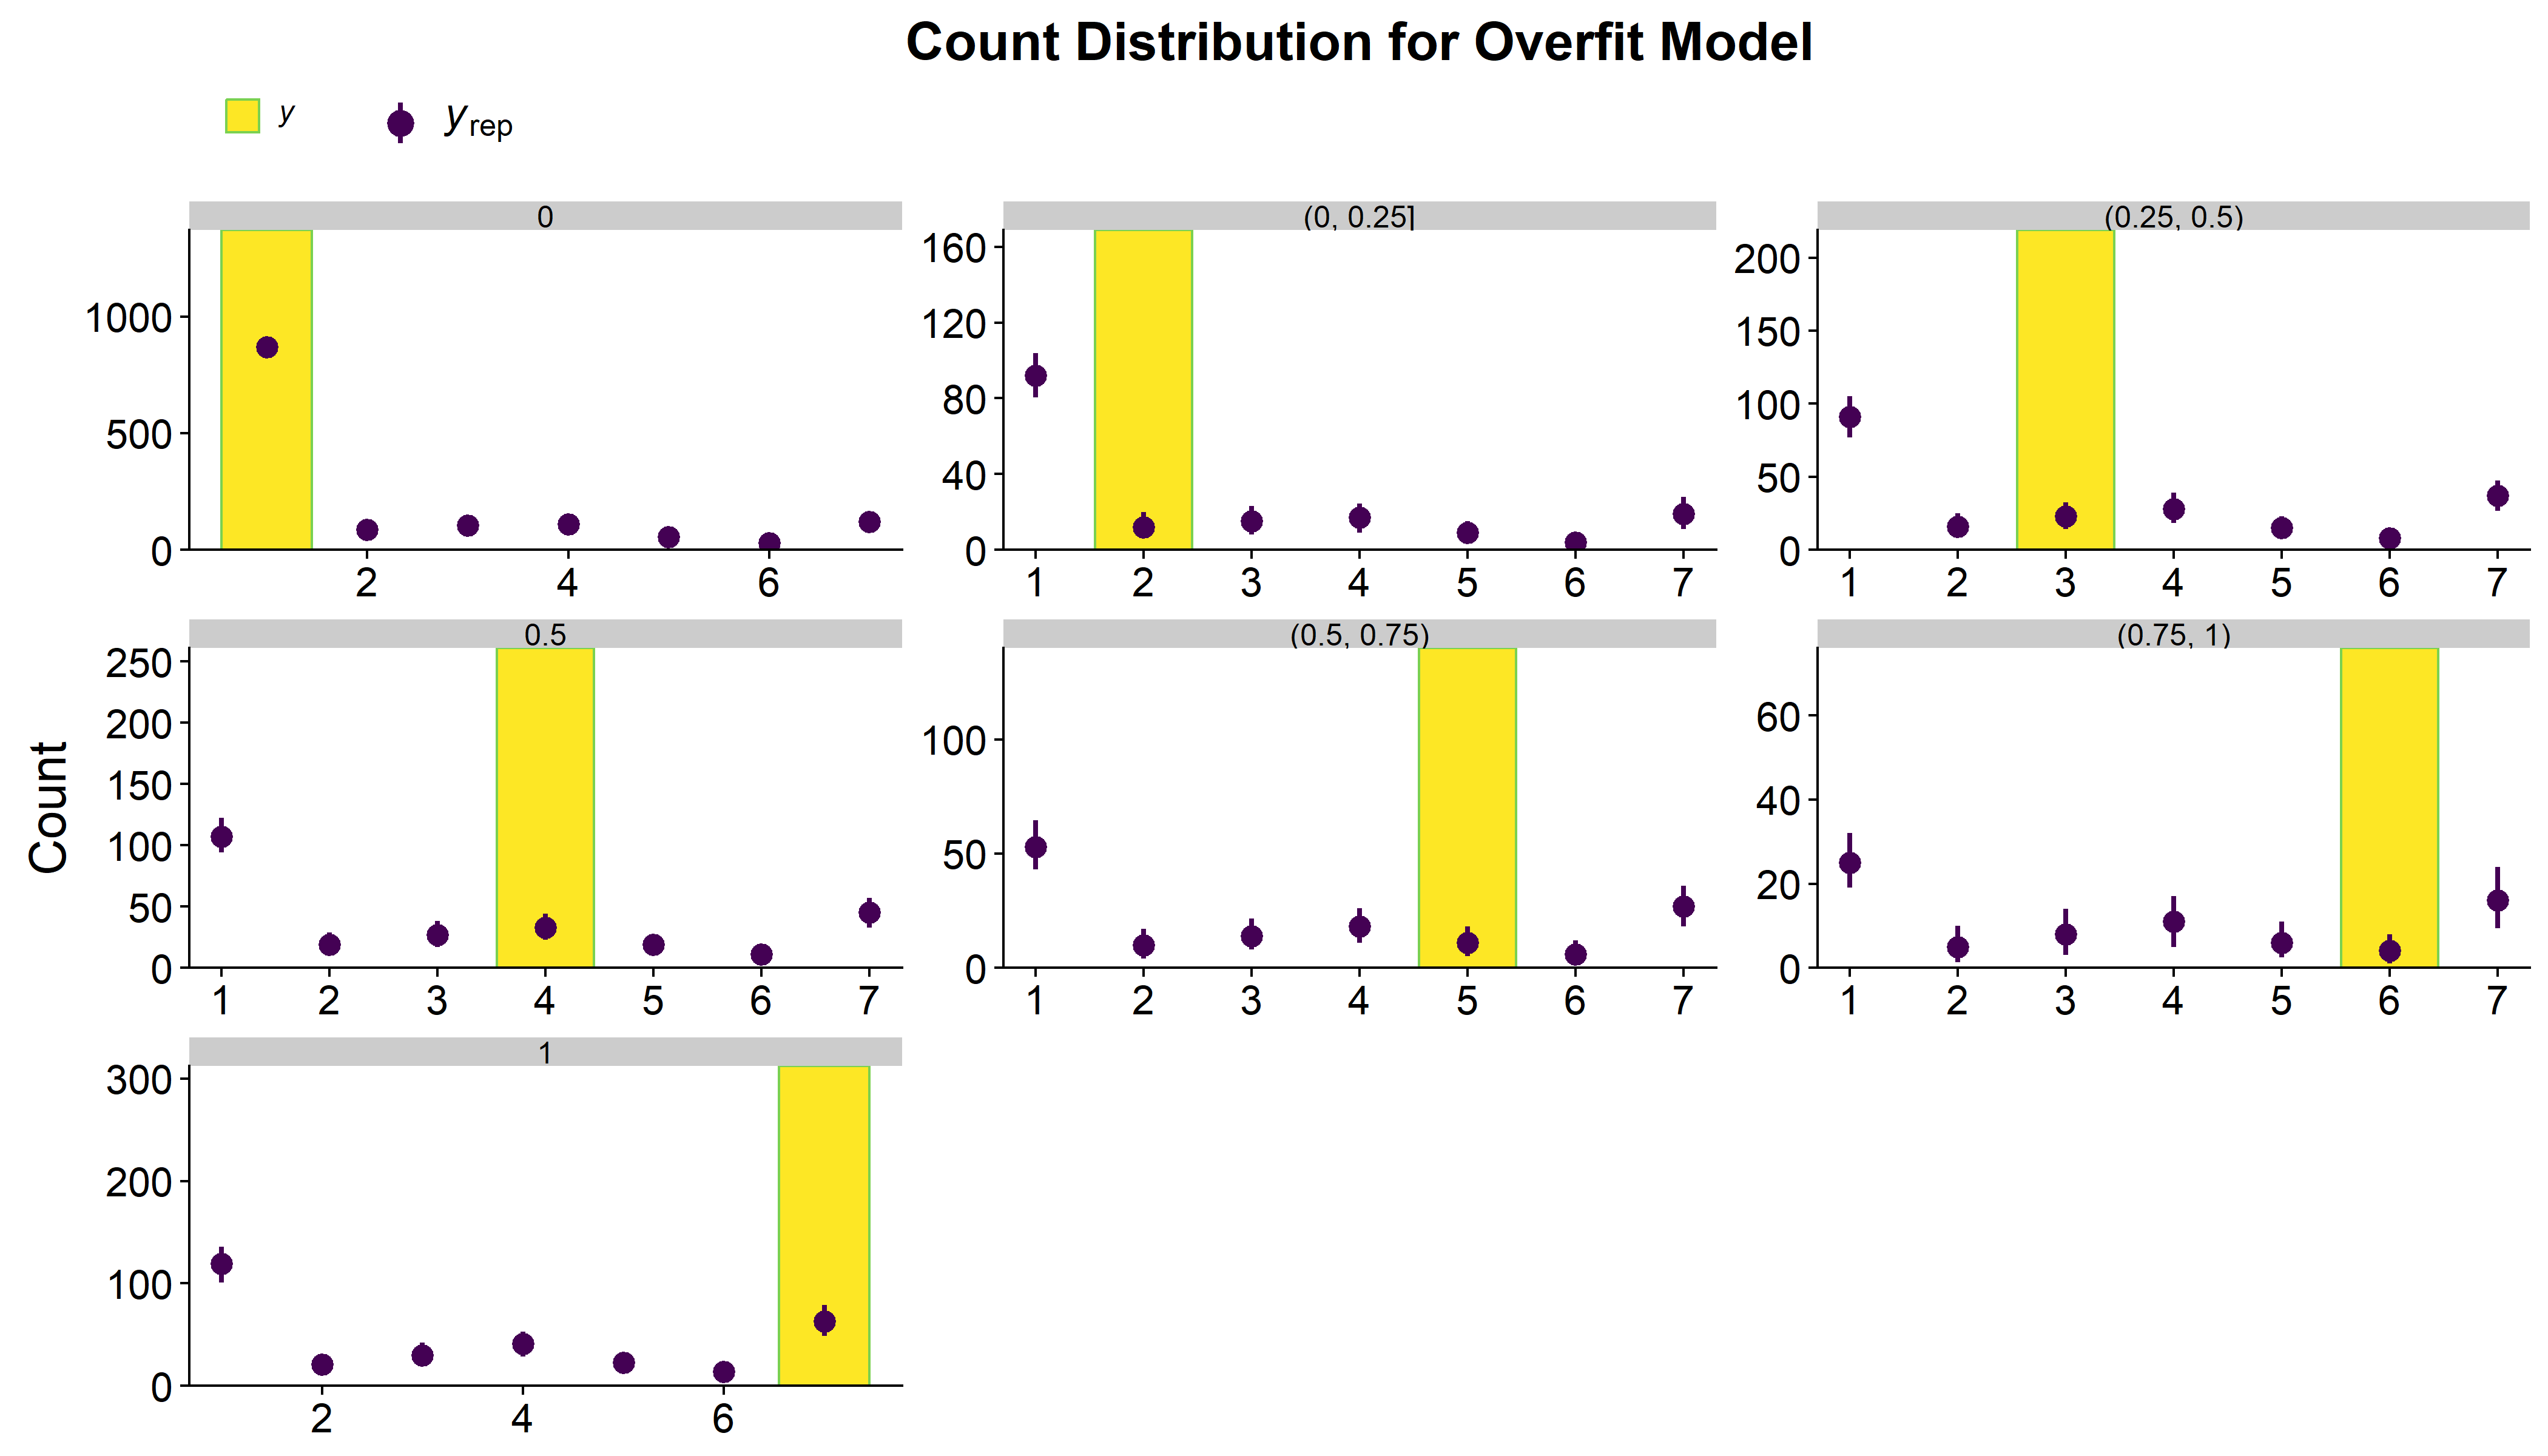
\includegraphics[width = 0.7\textwidth, height = 0.37\textheight]{Figures/3_2_Overfit_Preds.png}
	\caption{Frequencies vs True Values (Overfit)} \label{fig::3_Overfit_PredPlot}	
\end{figure}

\begin{figure}[h!]
	\centering
	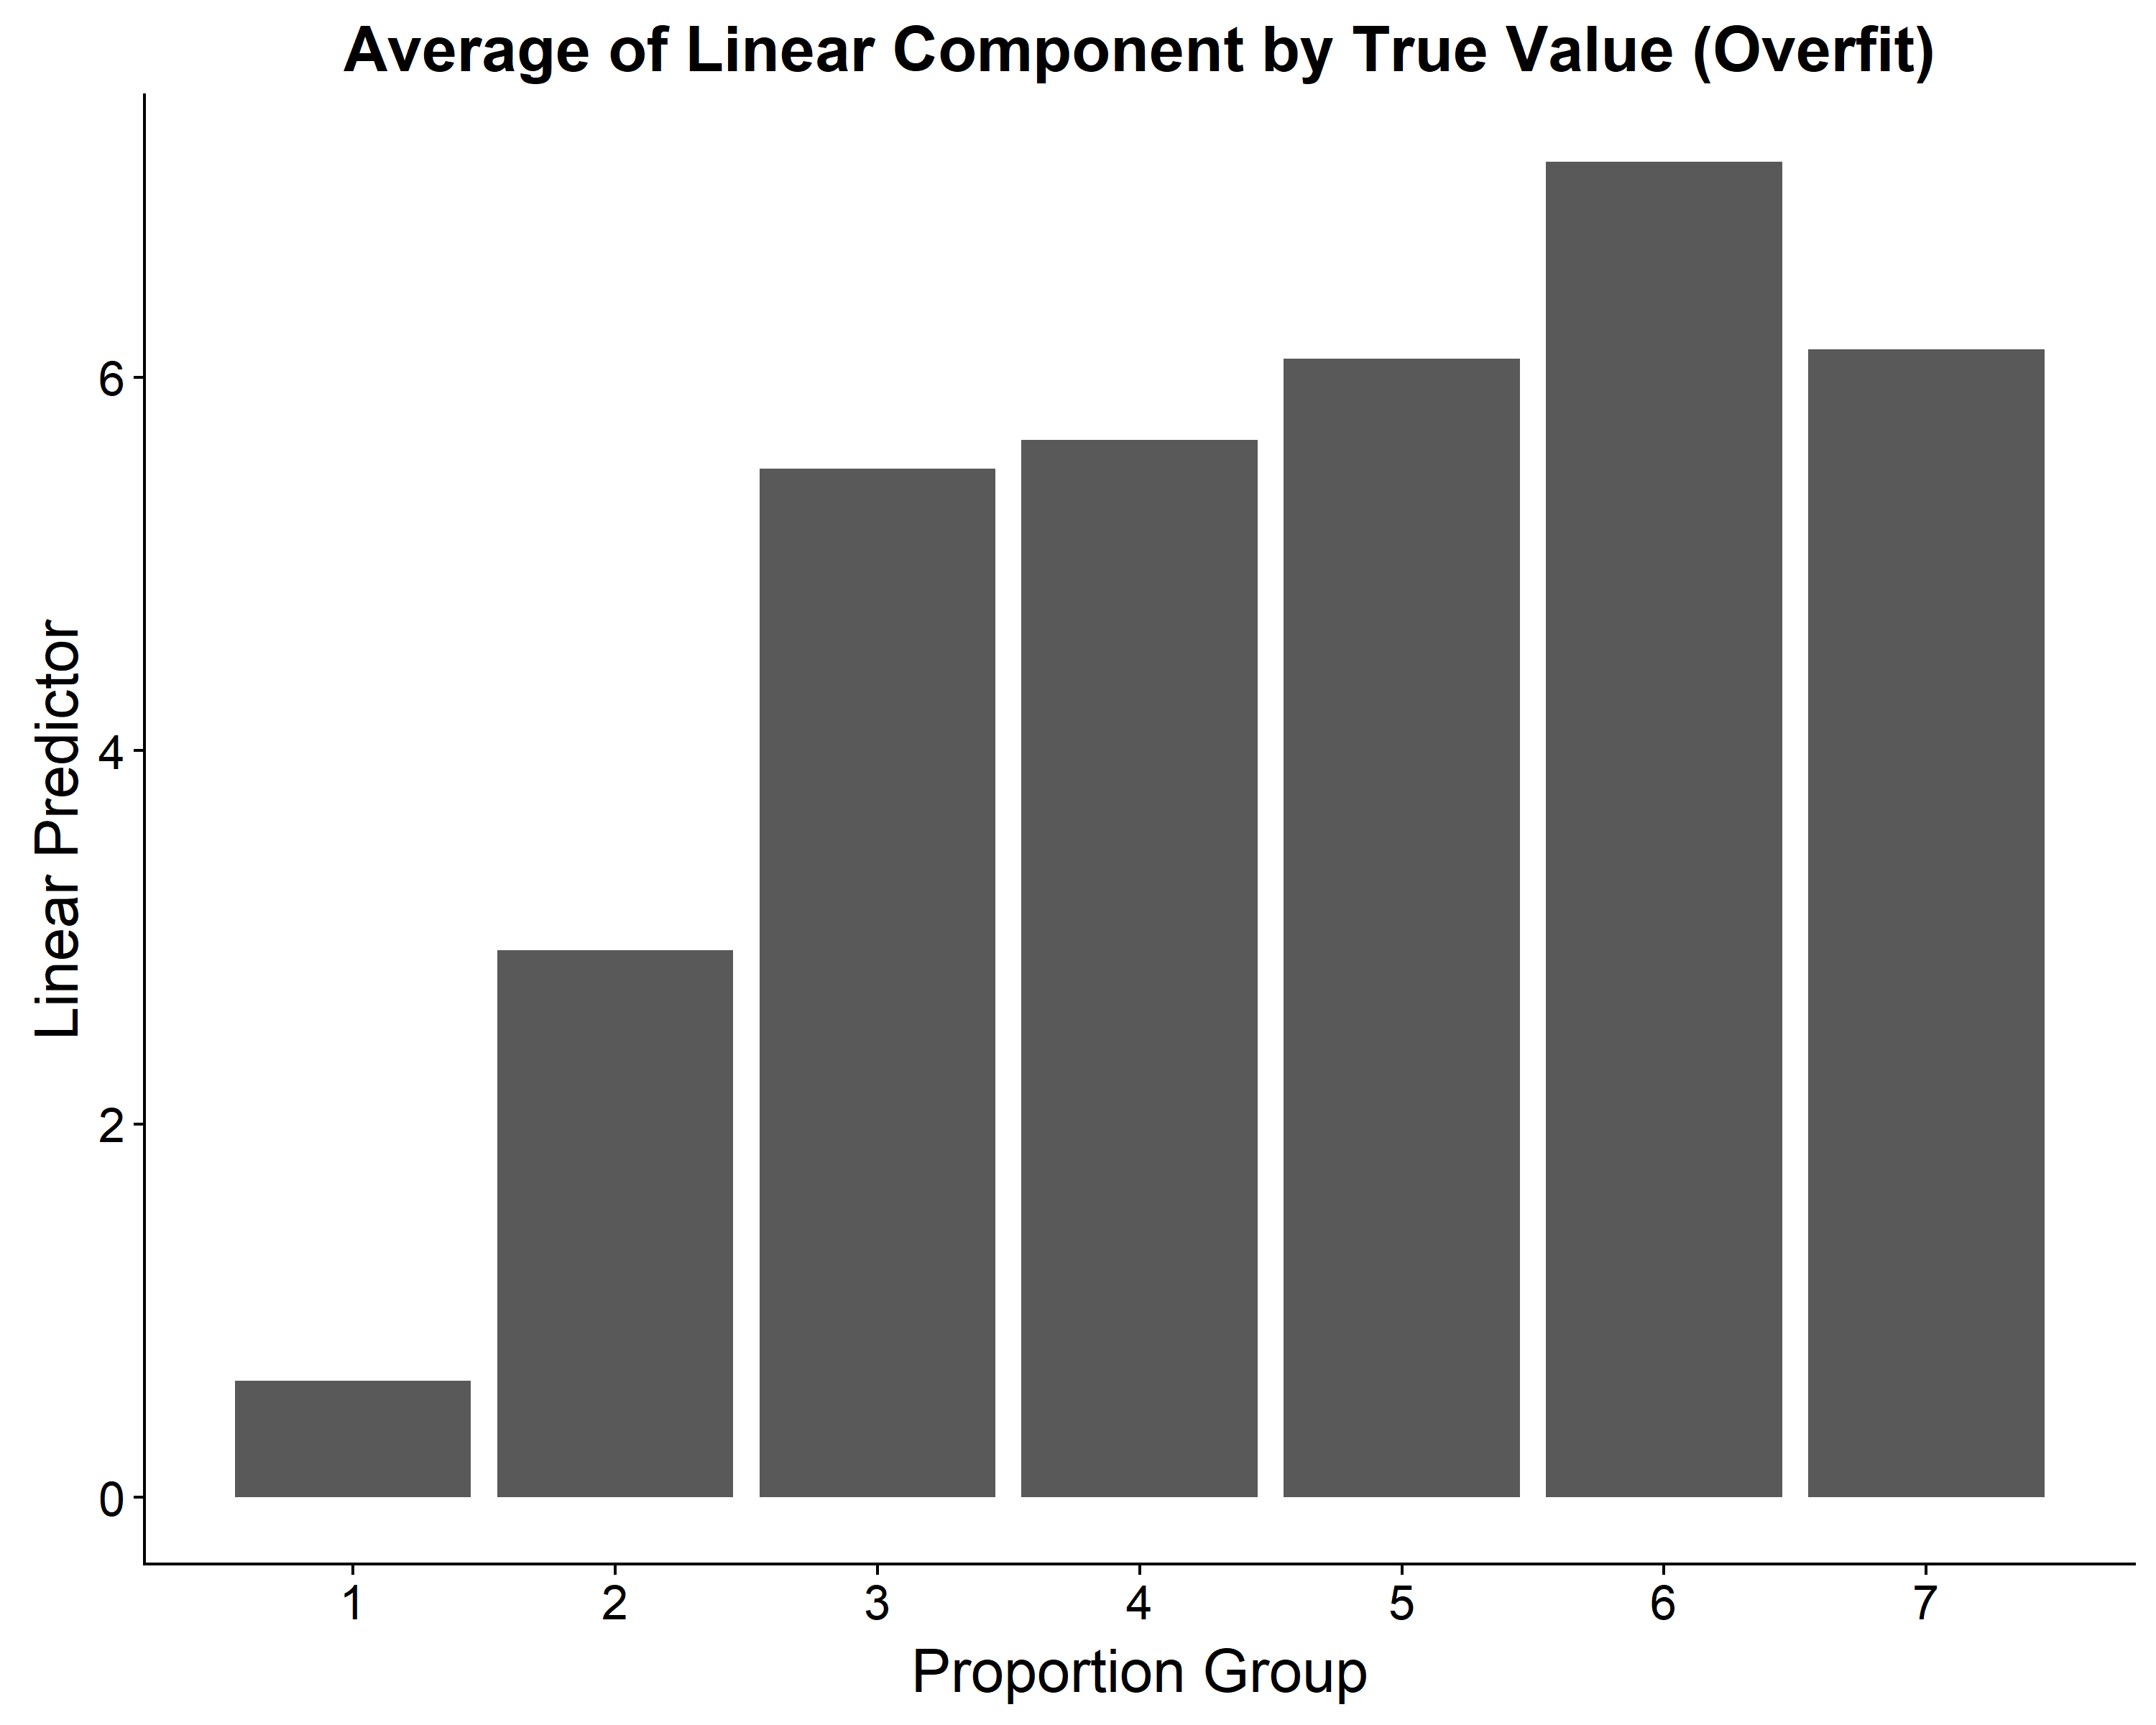
\includegraphics[height = 0.4\textheight]{Figures/3_2_Overfit_LinPreds.png}
	\caption{Linear Predictor vs True (Overfit)} \label{fig::3_Overfit_LinPredPlot}	
\end{figure}



\clearpage

\newpage
\subsection{Posterior Predictive (\texttt{mc41})}


First, consider Figure \ref{fig::4_MC41_BarClass}. Though at first glance there are many ``wrong" estimates (e.g. the top left panel), this is just a result of shrinkage to the mean that comes with using group-level effects. Since there are not many obserations in certain groups, their intercept is pushed towards the mean as a result of the common distribution shared by each group. This is how varying intercepts/slopes prevent overfitting in hierarchical models. \cite{McElreath_book} refers to this as adaptive regularisation. See also \cite{GelmanBDA2013}, or \cite{GelmanHill2007}. 

The ECDF in Figure \ref{fig::4_MC41_ECDF} looks to fit the data well. 

The test statistics for 0s, 1s, and 0.5s in Figures \ref{fig::4_MC41_Zeros}, \ref{fig::4_MC41_Ones}, and \ref{fig::4_MC41_Ones} largely seem appropriate. Some exceptions are the number of 1s for vancomycin, and possibly flucloxacillin, and the numbers of 0.5s for vancomycin, cefalexin, ceftriaxone, and ciprofloxacin. 

The barplot of frequencies against true values (Figure \ref{fig::4_MC41_BarPred}), and the latent variable plot (Figure \ref{fig::4_MC41_LinPred}) are the same story as previously. Poor actual predictions, but a mostly desirable pattern in the latent variable. 

\begin{figure}[h!]
	\centering
	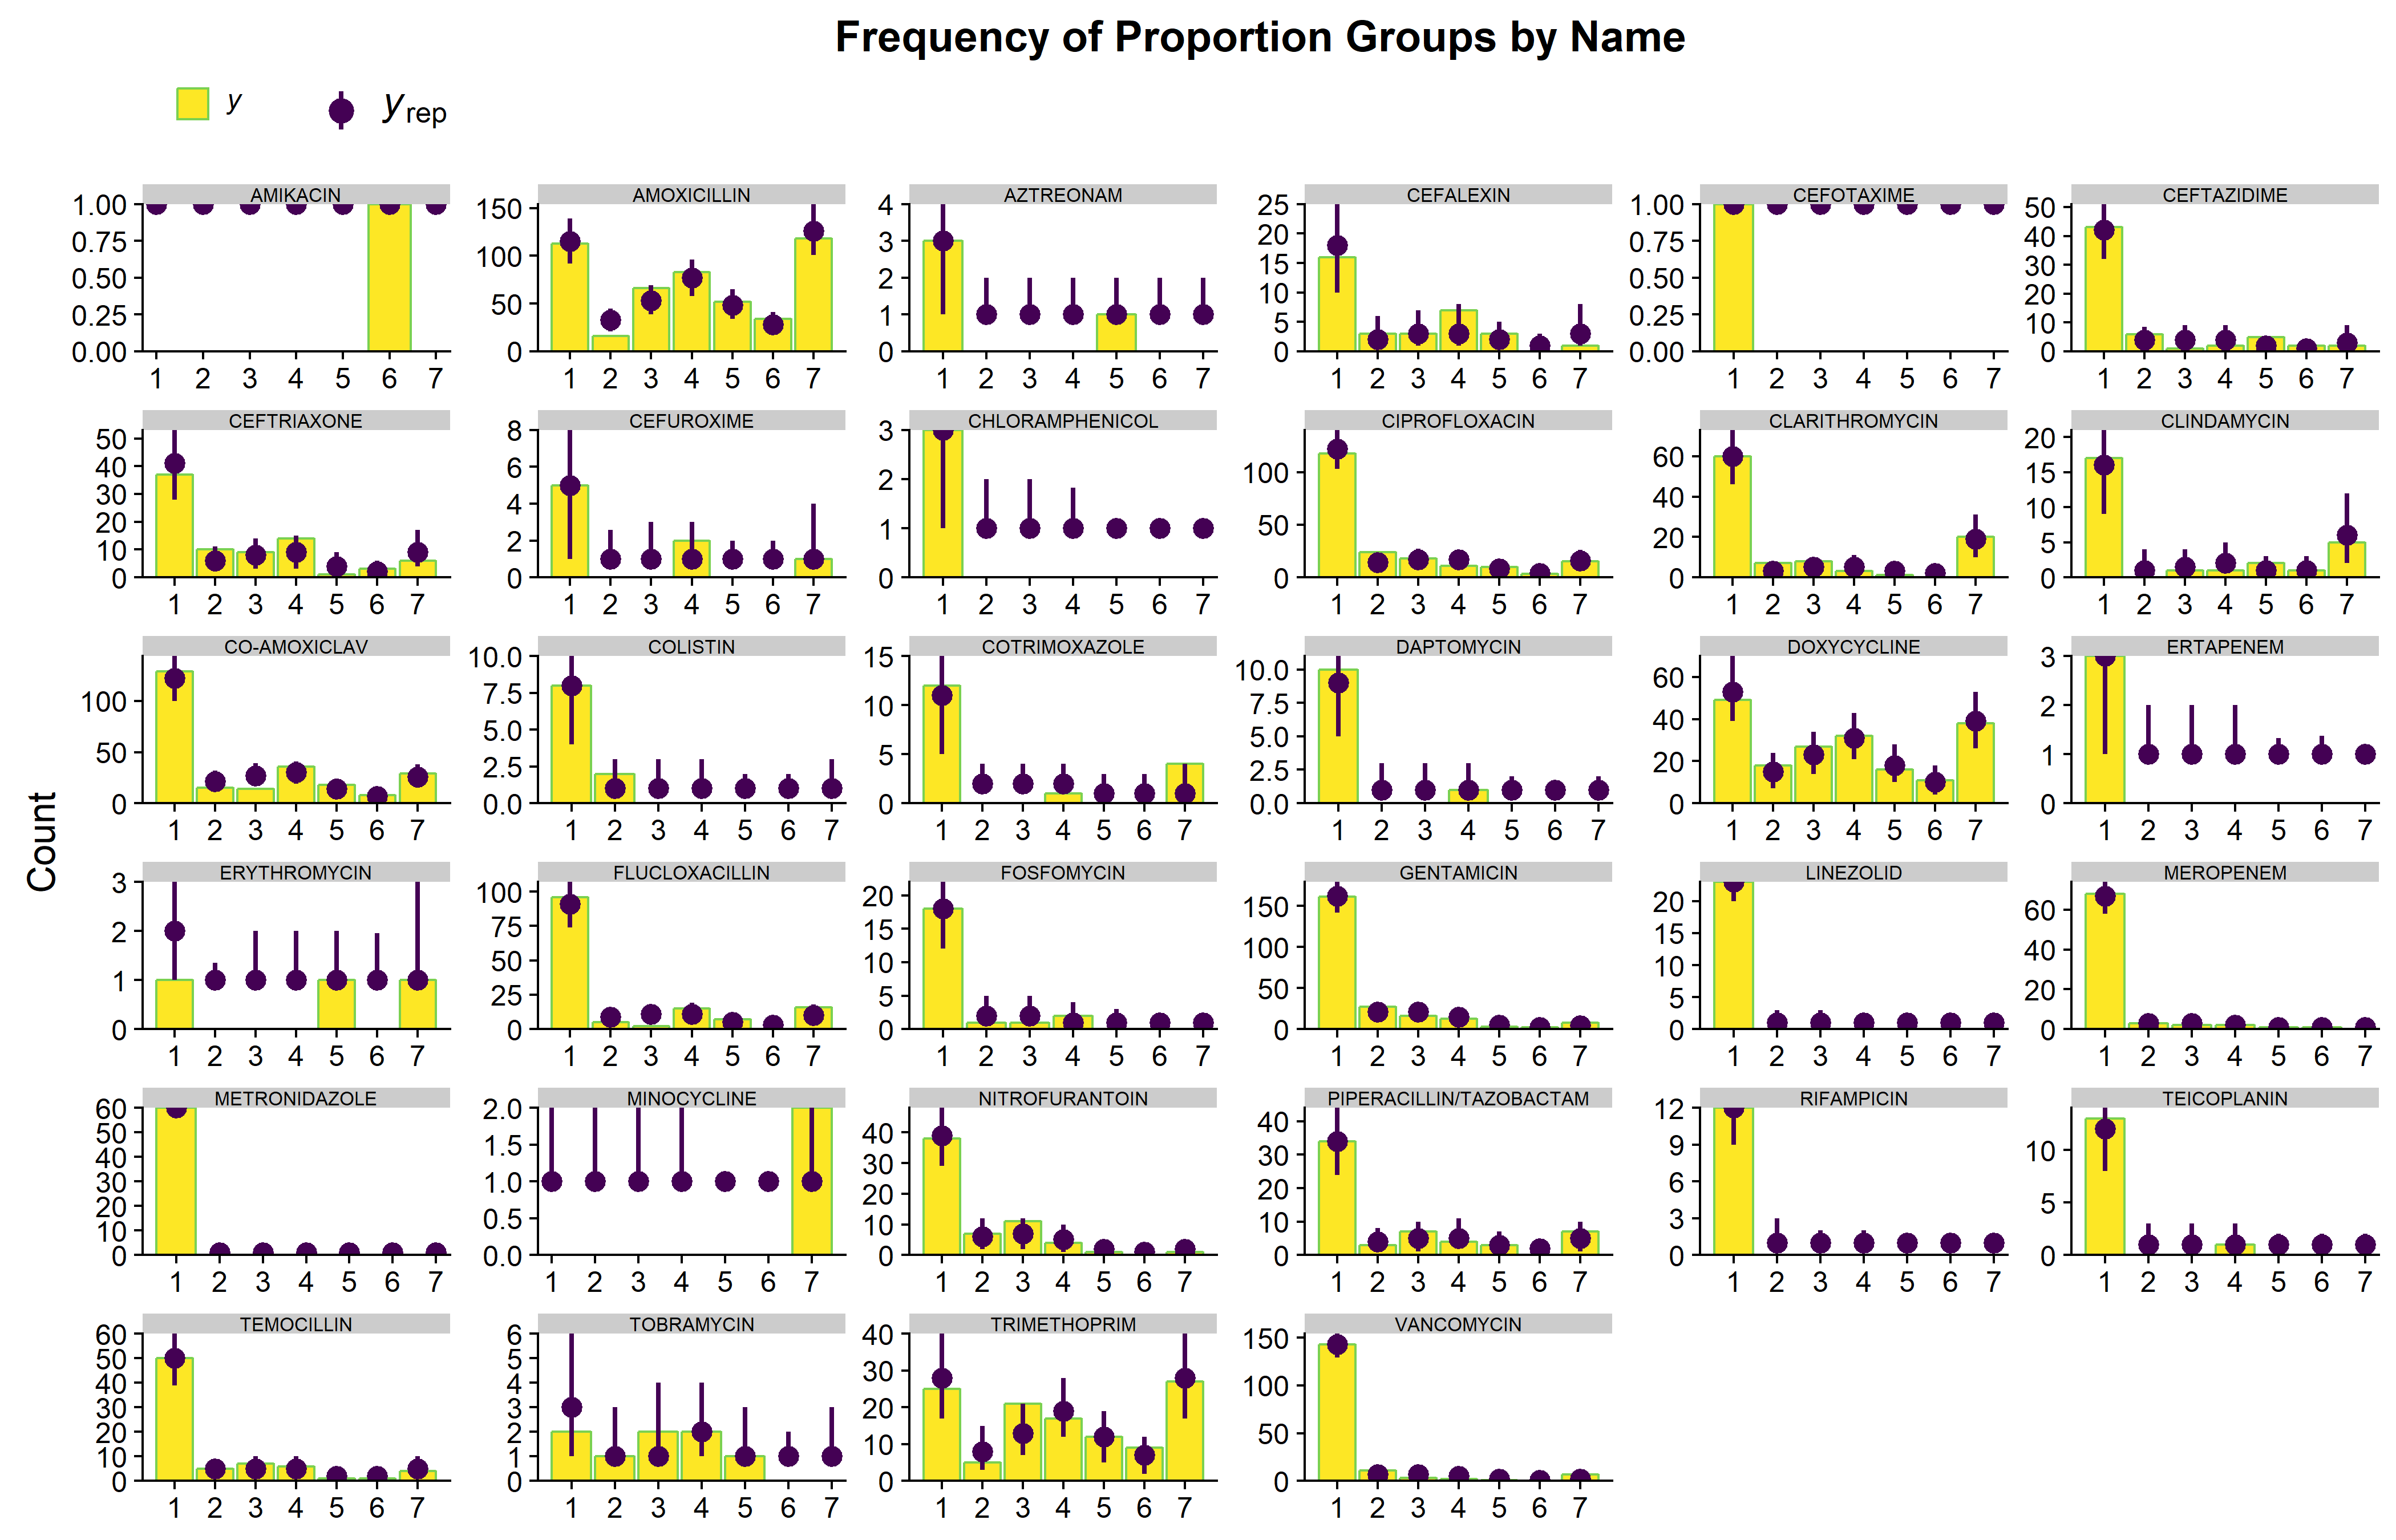
\includegraphics[width = 0.95\textwidth, height = 0.60\textheight]{Figures/4_MC41_BarClass.png}
	\caption{Frequency by Name} \label{fig::4_MC41_BarClass}	
\end{figure}

\newpage

\begin{figure}[h!]
	\centering
	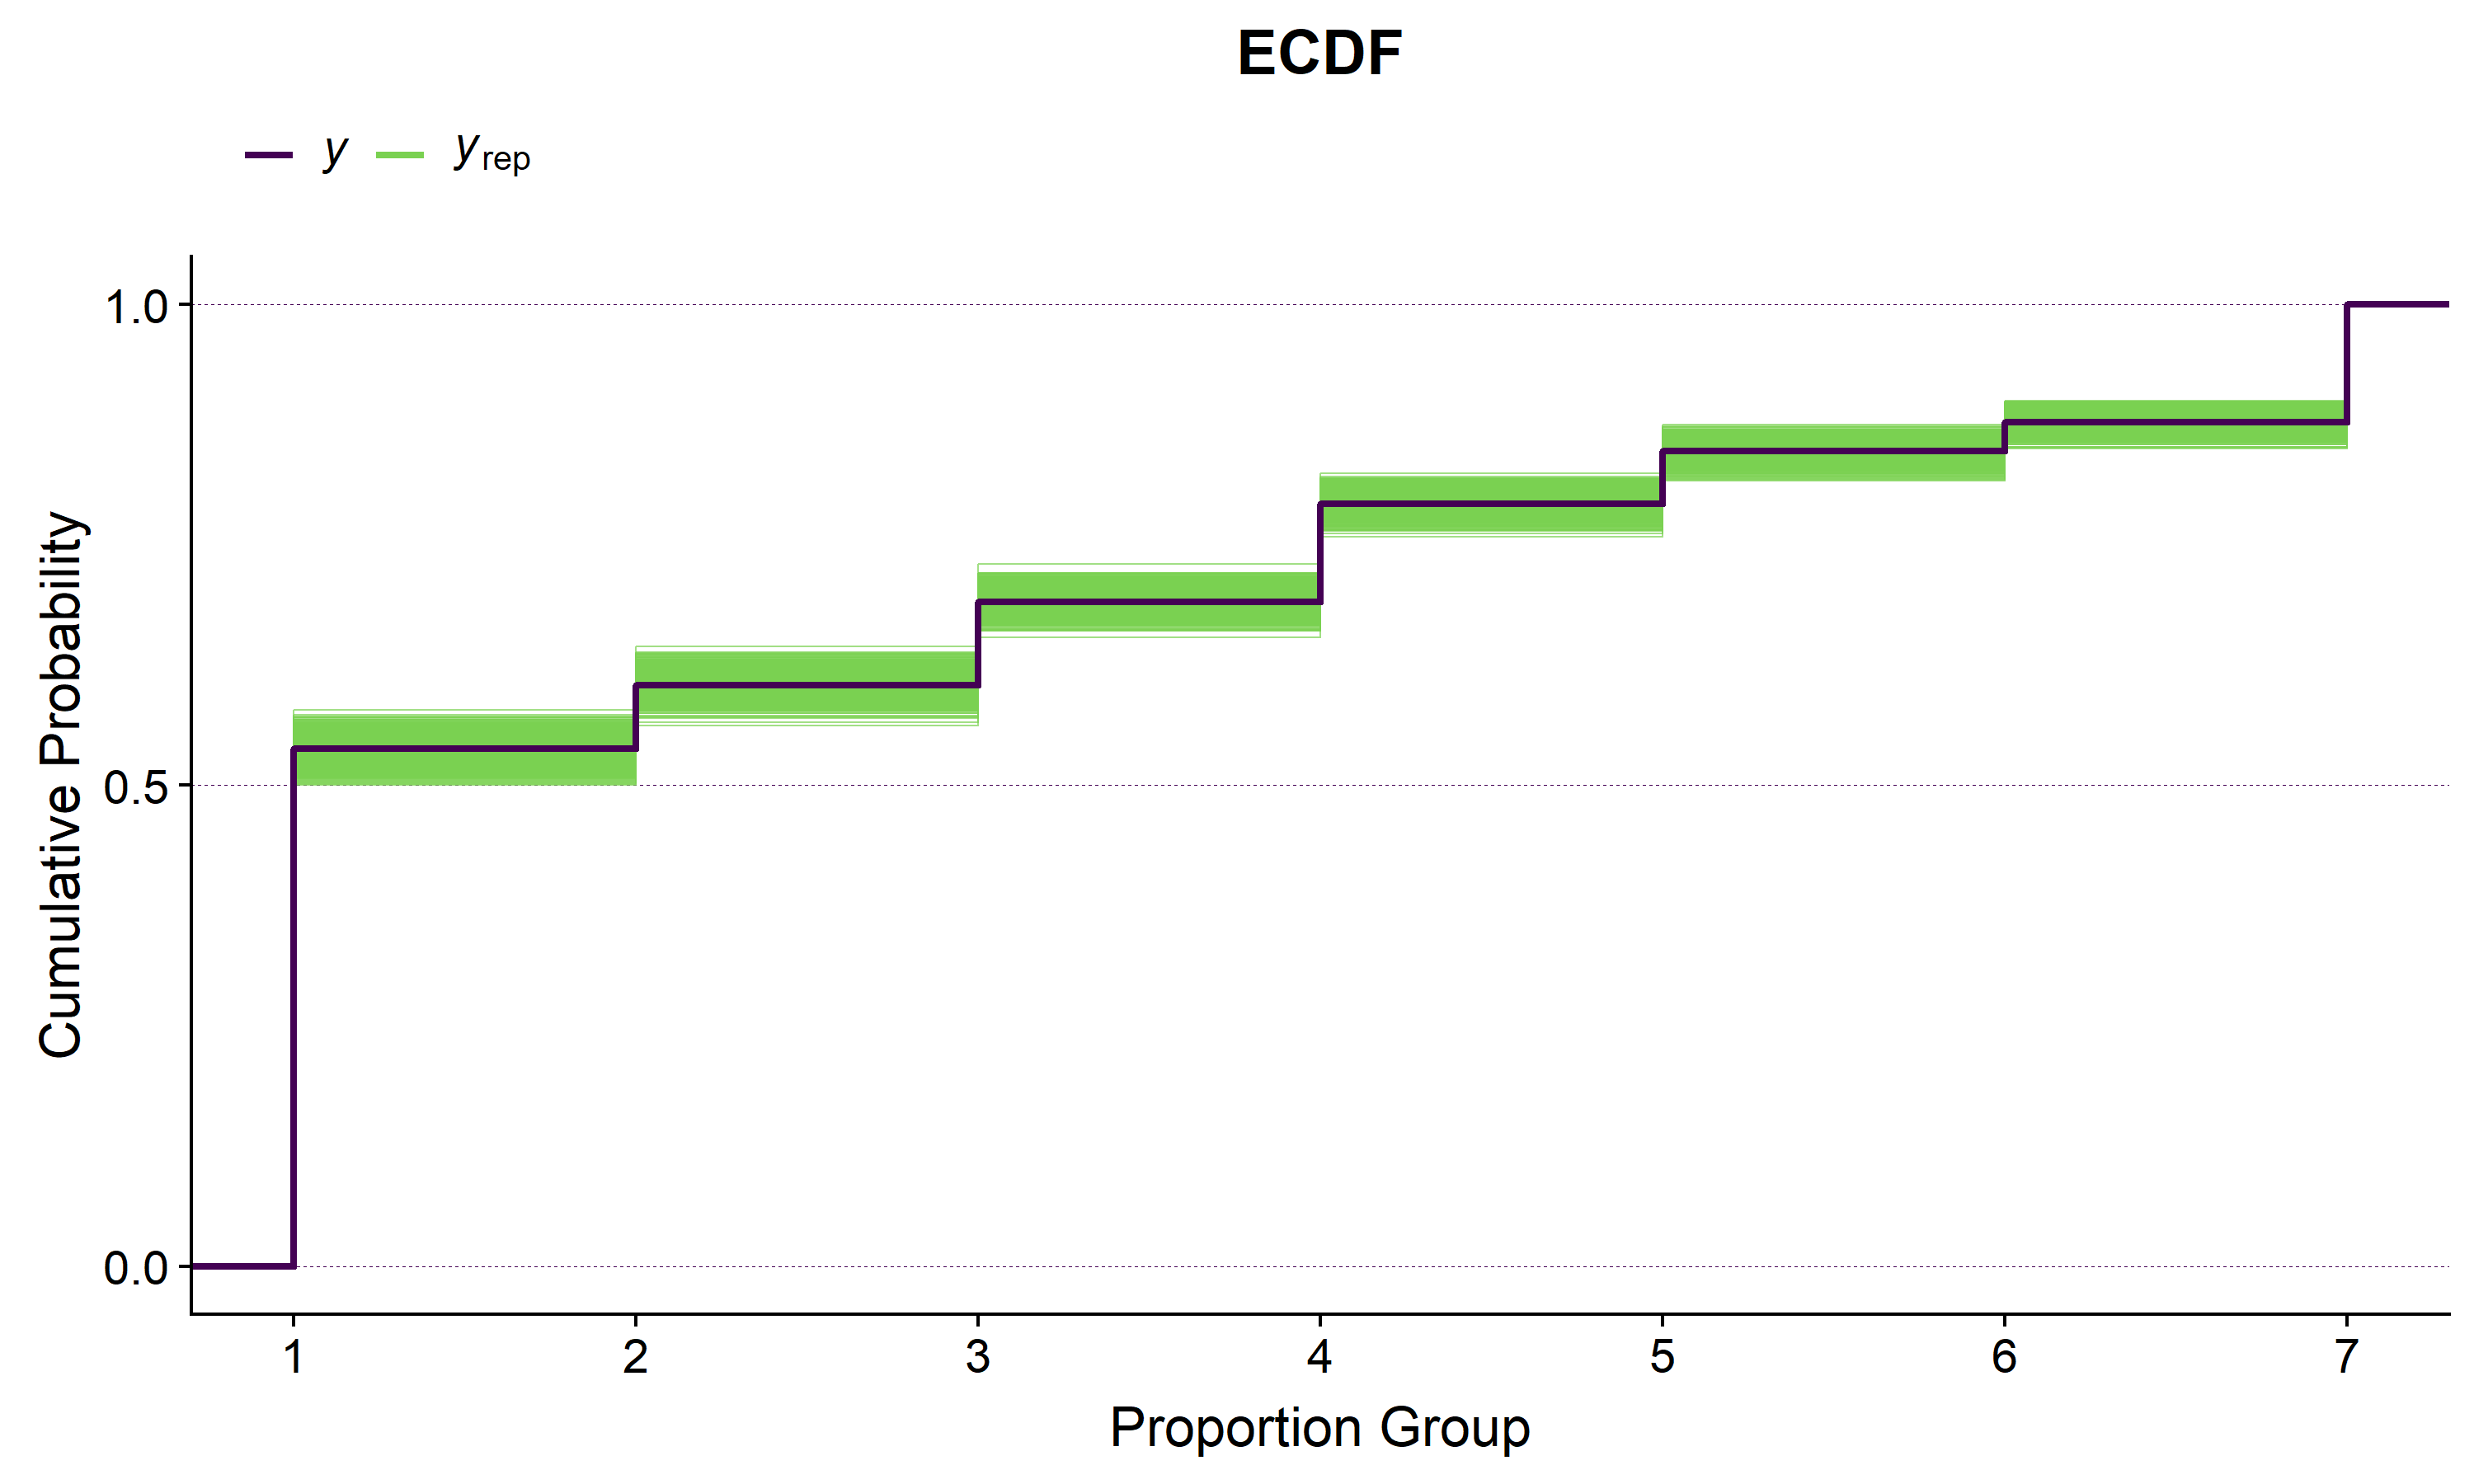
\includegraphics[height = 0.35\textheight]{Figures/4_MC41_ECDF.png}
	\caption{ECDF} \label{fig::4_MC41_ECDF}	
\end{figure}

\begin{figure}[h!]
	\centering
	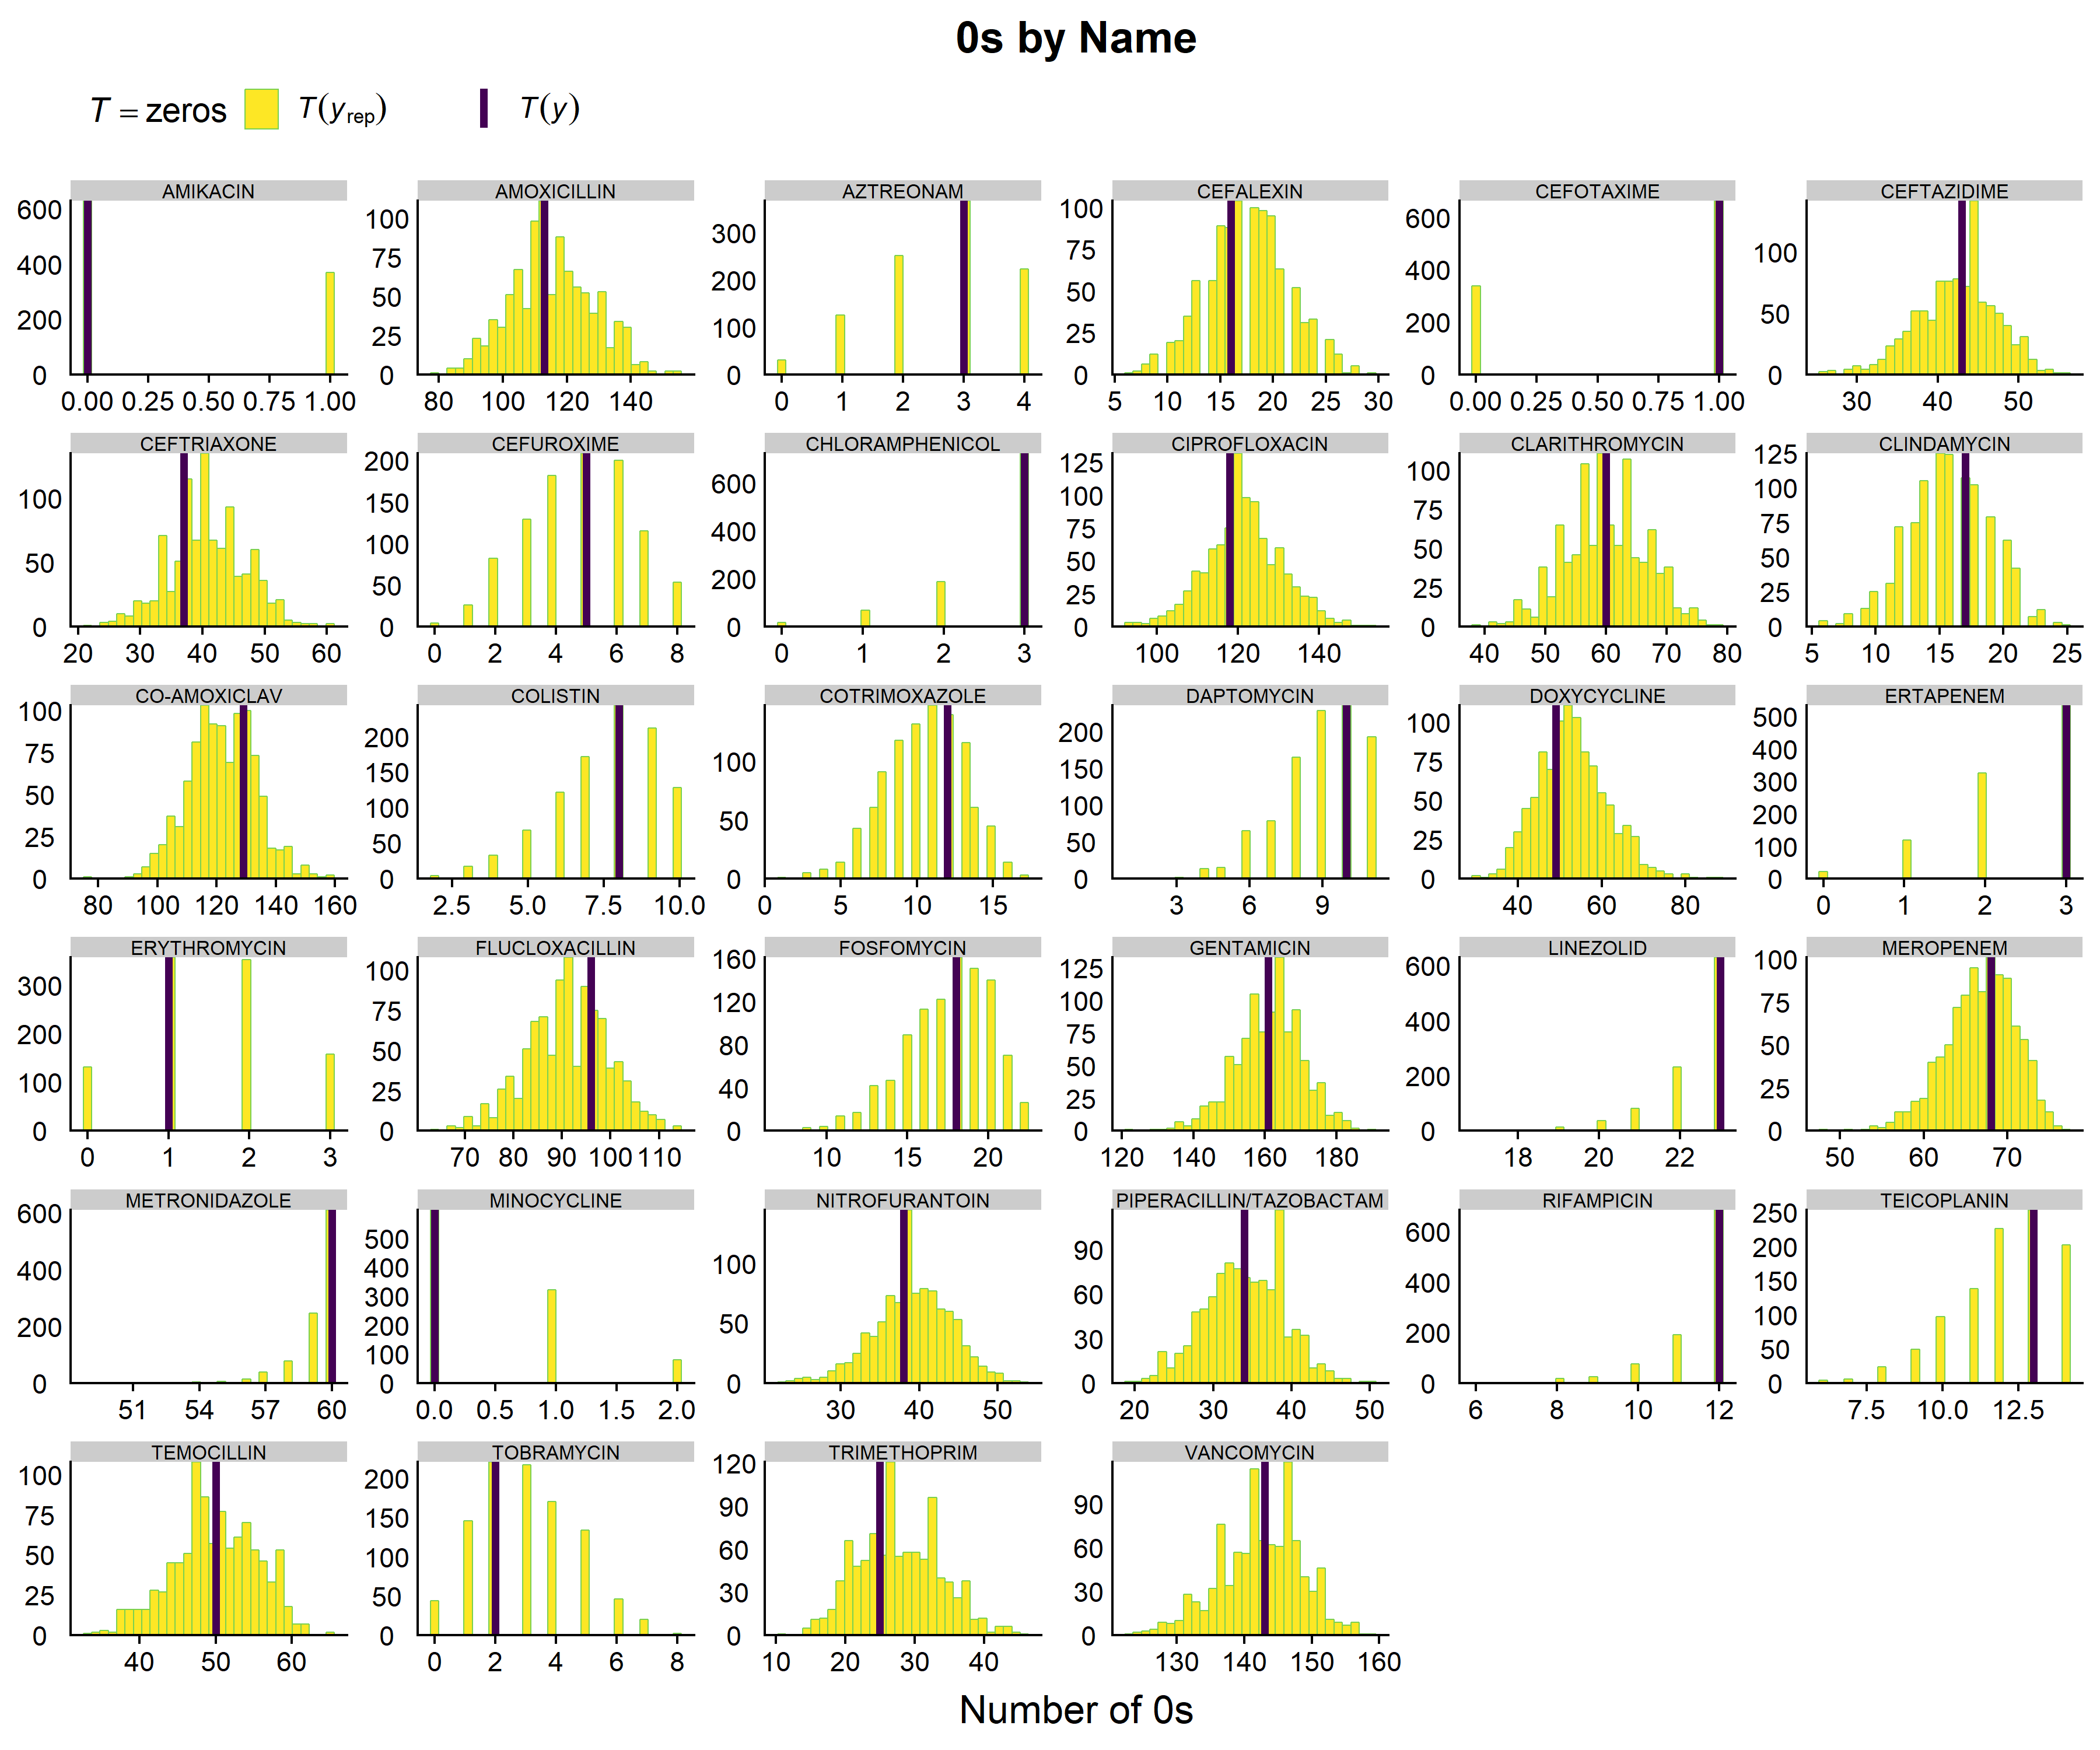
\includegraphics[width = 1\textwidth, height=0.5\textheight]{Figures/4_MC41_Zeros.png}
	\caption{Test Statistic by Name (Number of 0s)} \label{fig::4_MC41_Zeros}	
\end{figure}


\begin{figure}[h!]
	\centering
	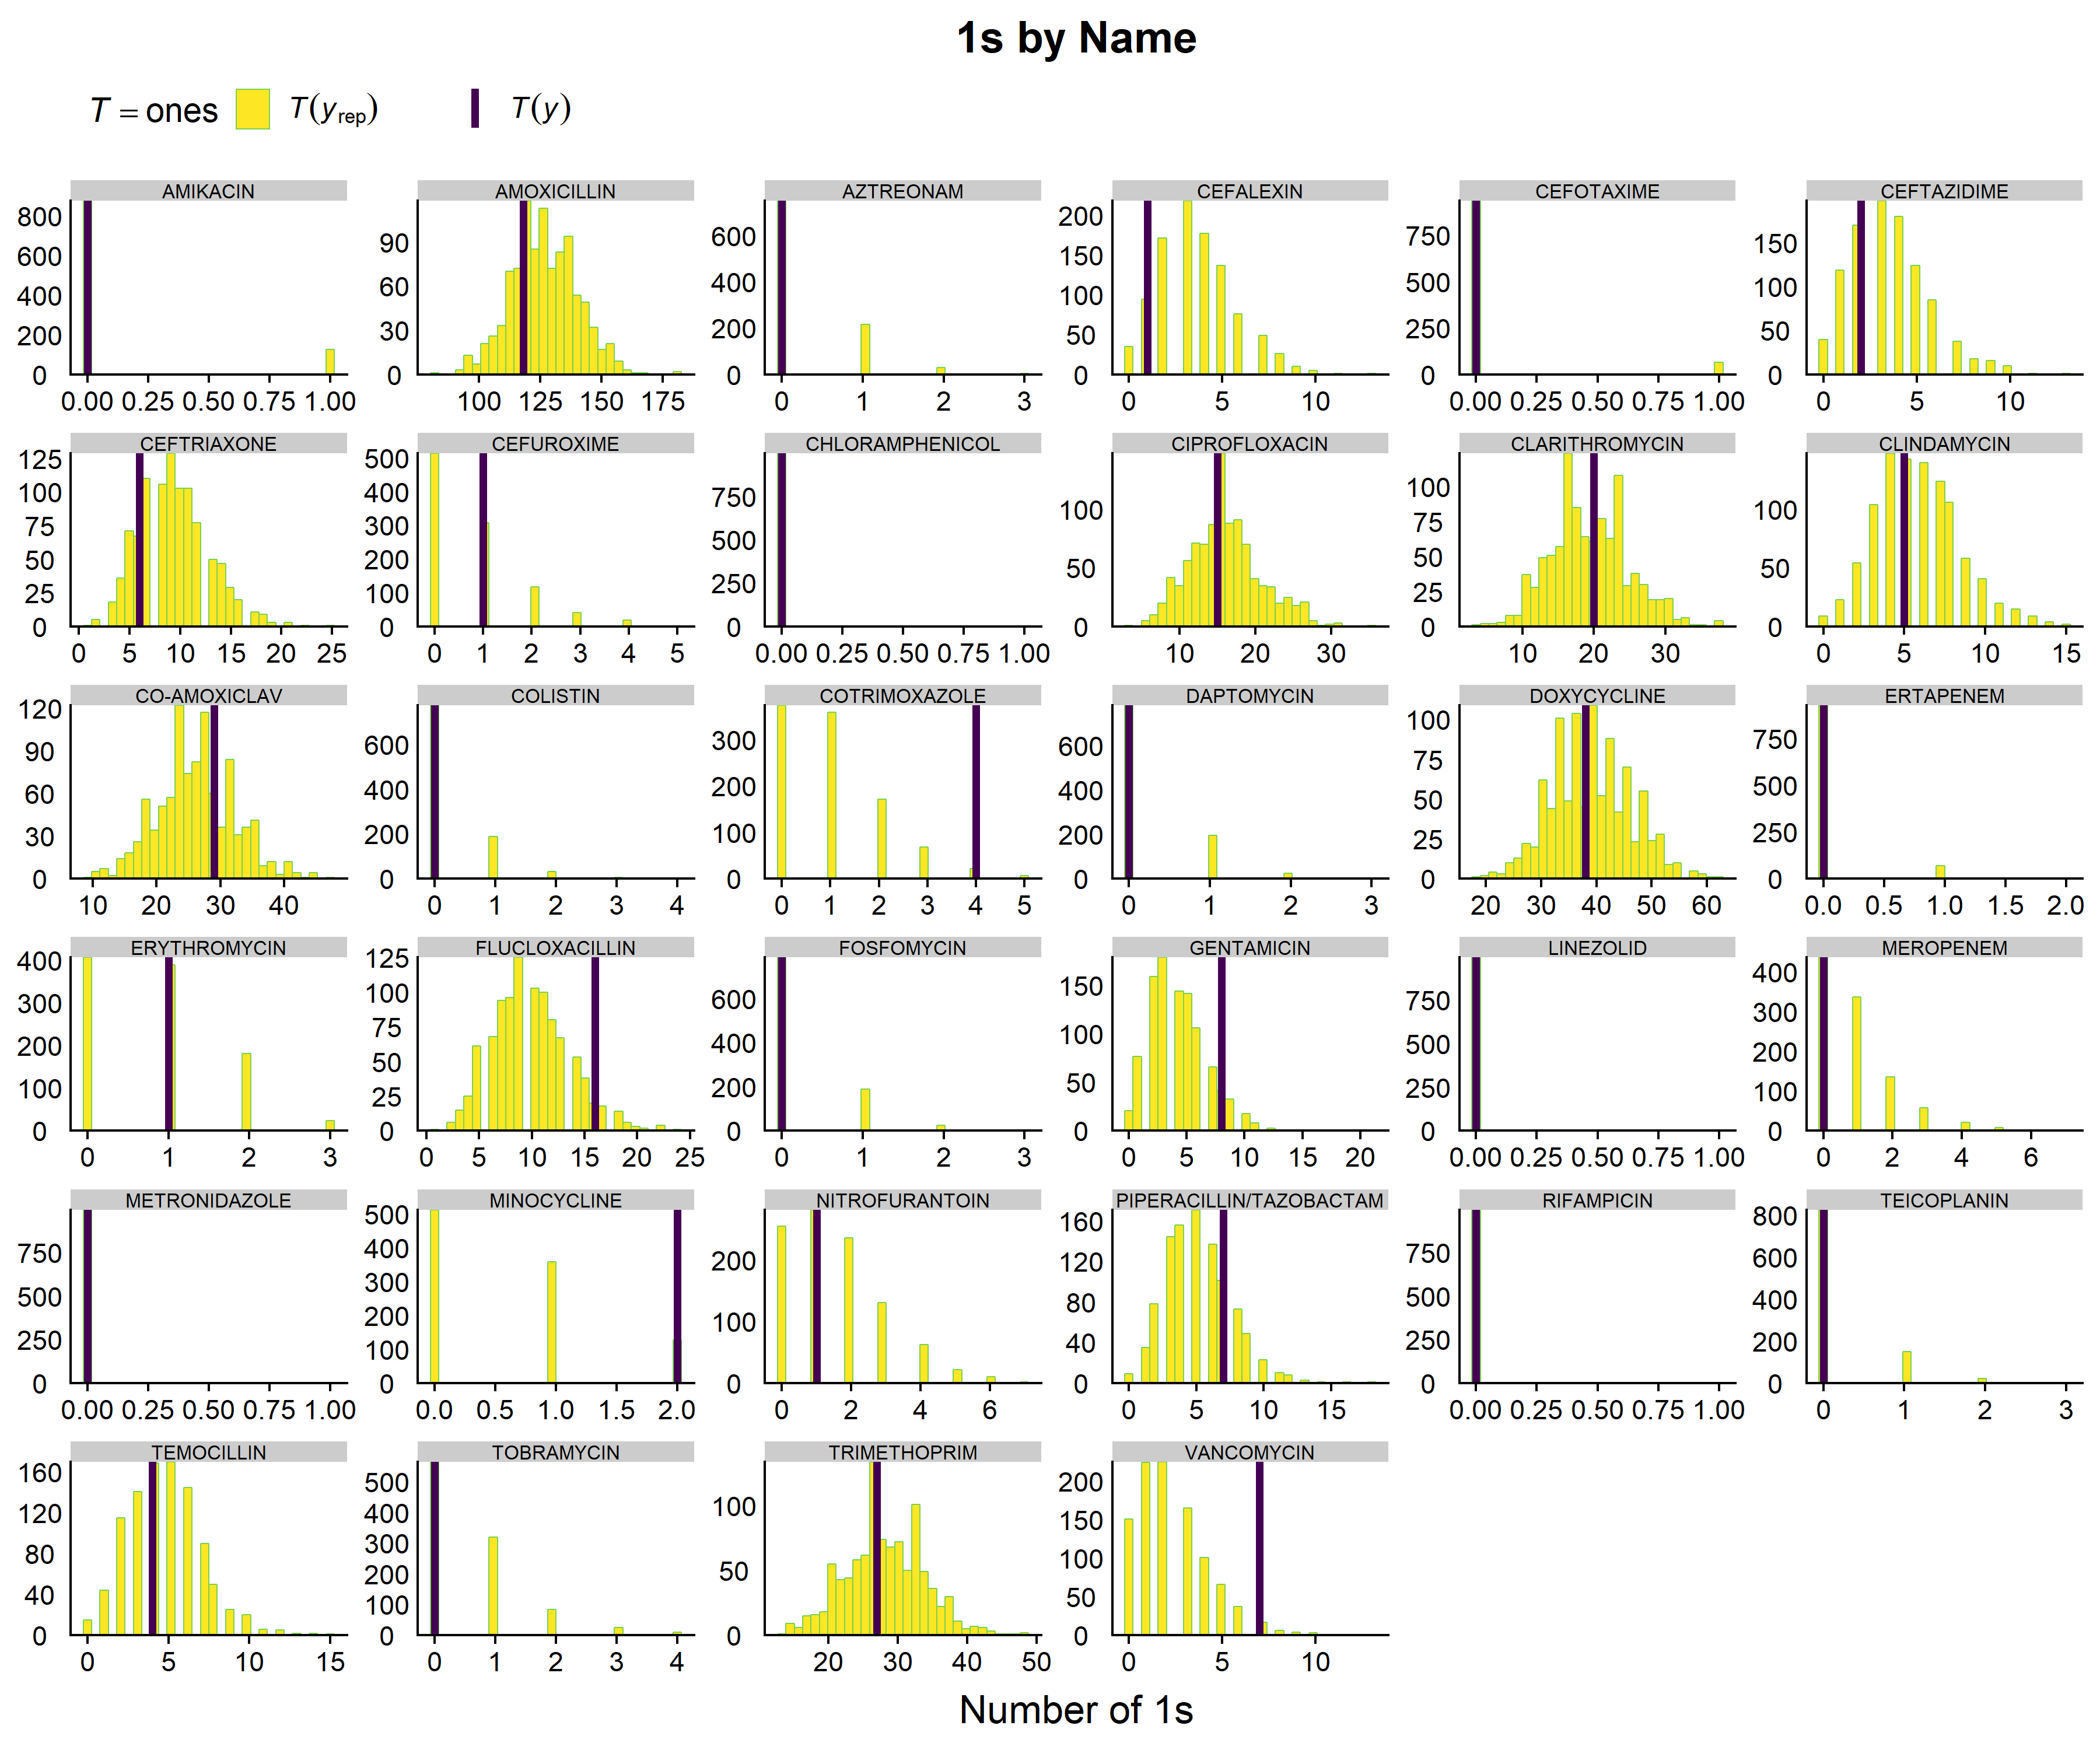
\includegraphics[width = 1\textwidth, height=0.45\textheight]{Figures/4_MC41_Ones.png}
	\caption{Test Statistic by Name (Number of 1s)} \label{fig::4_MC41_Ones}	
\end{figure}


\begin{figure}[h!]
	\centering
	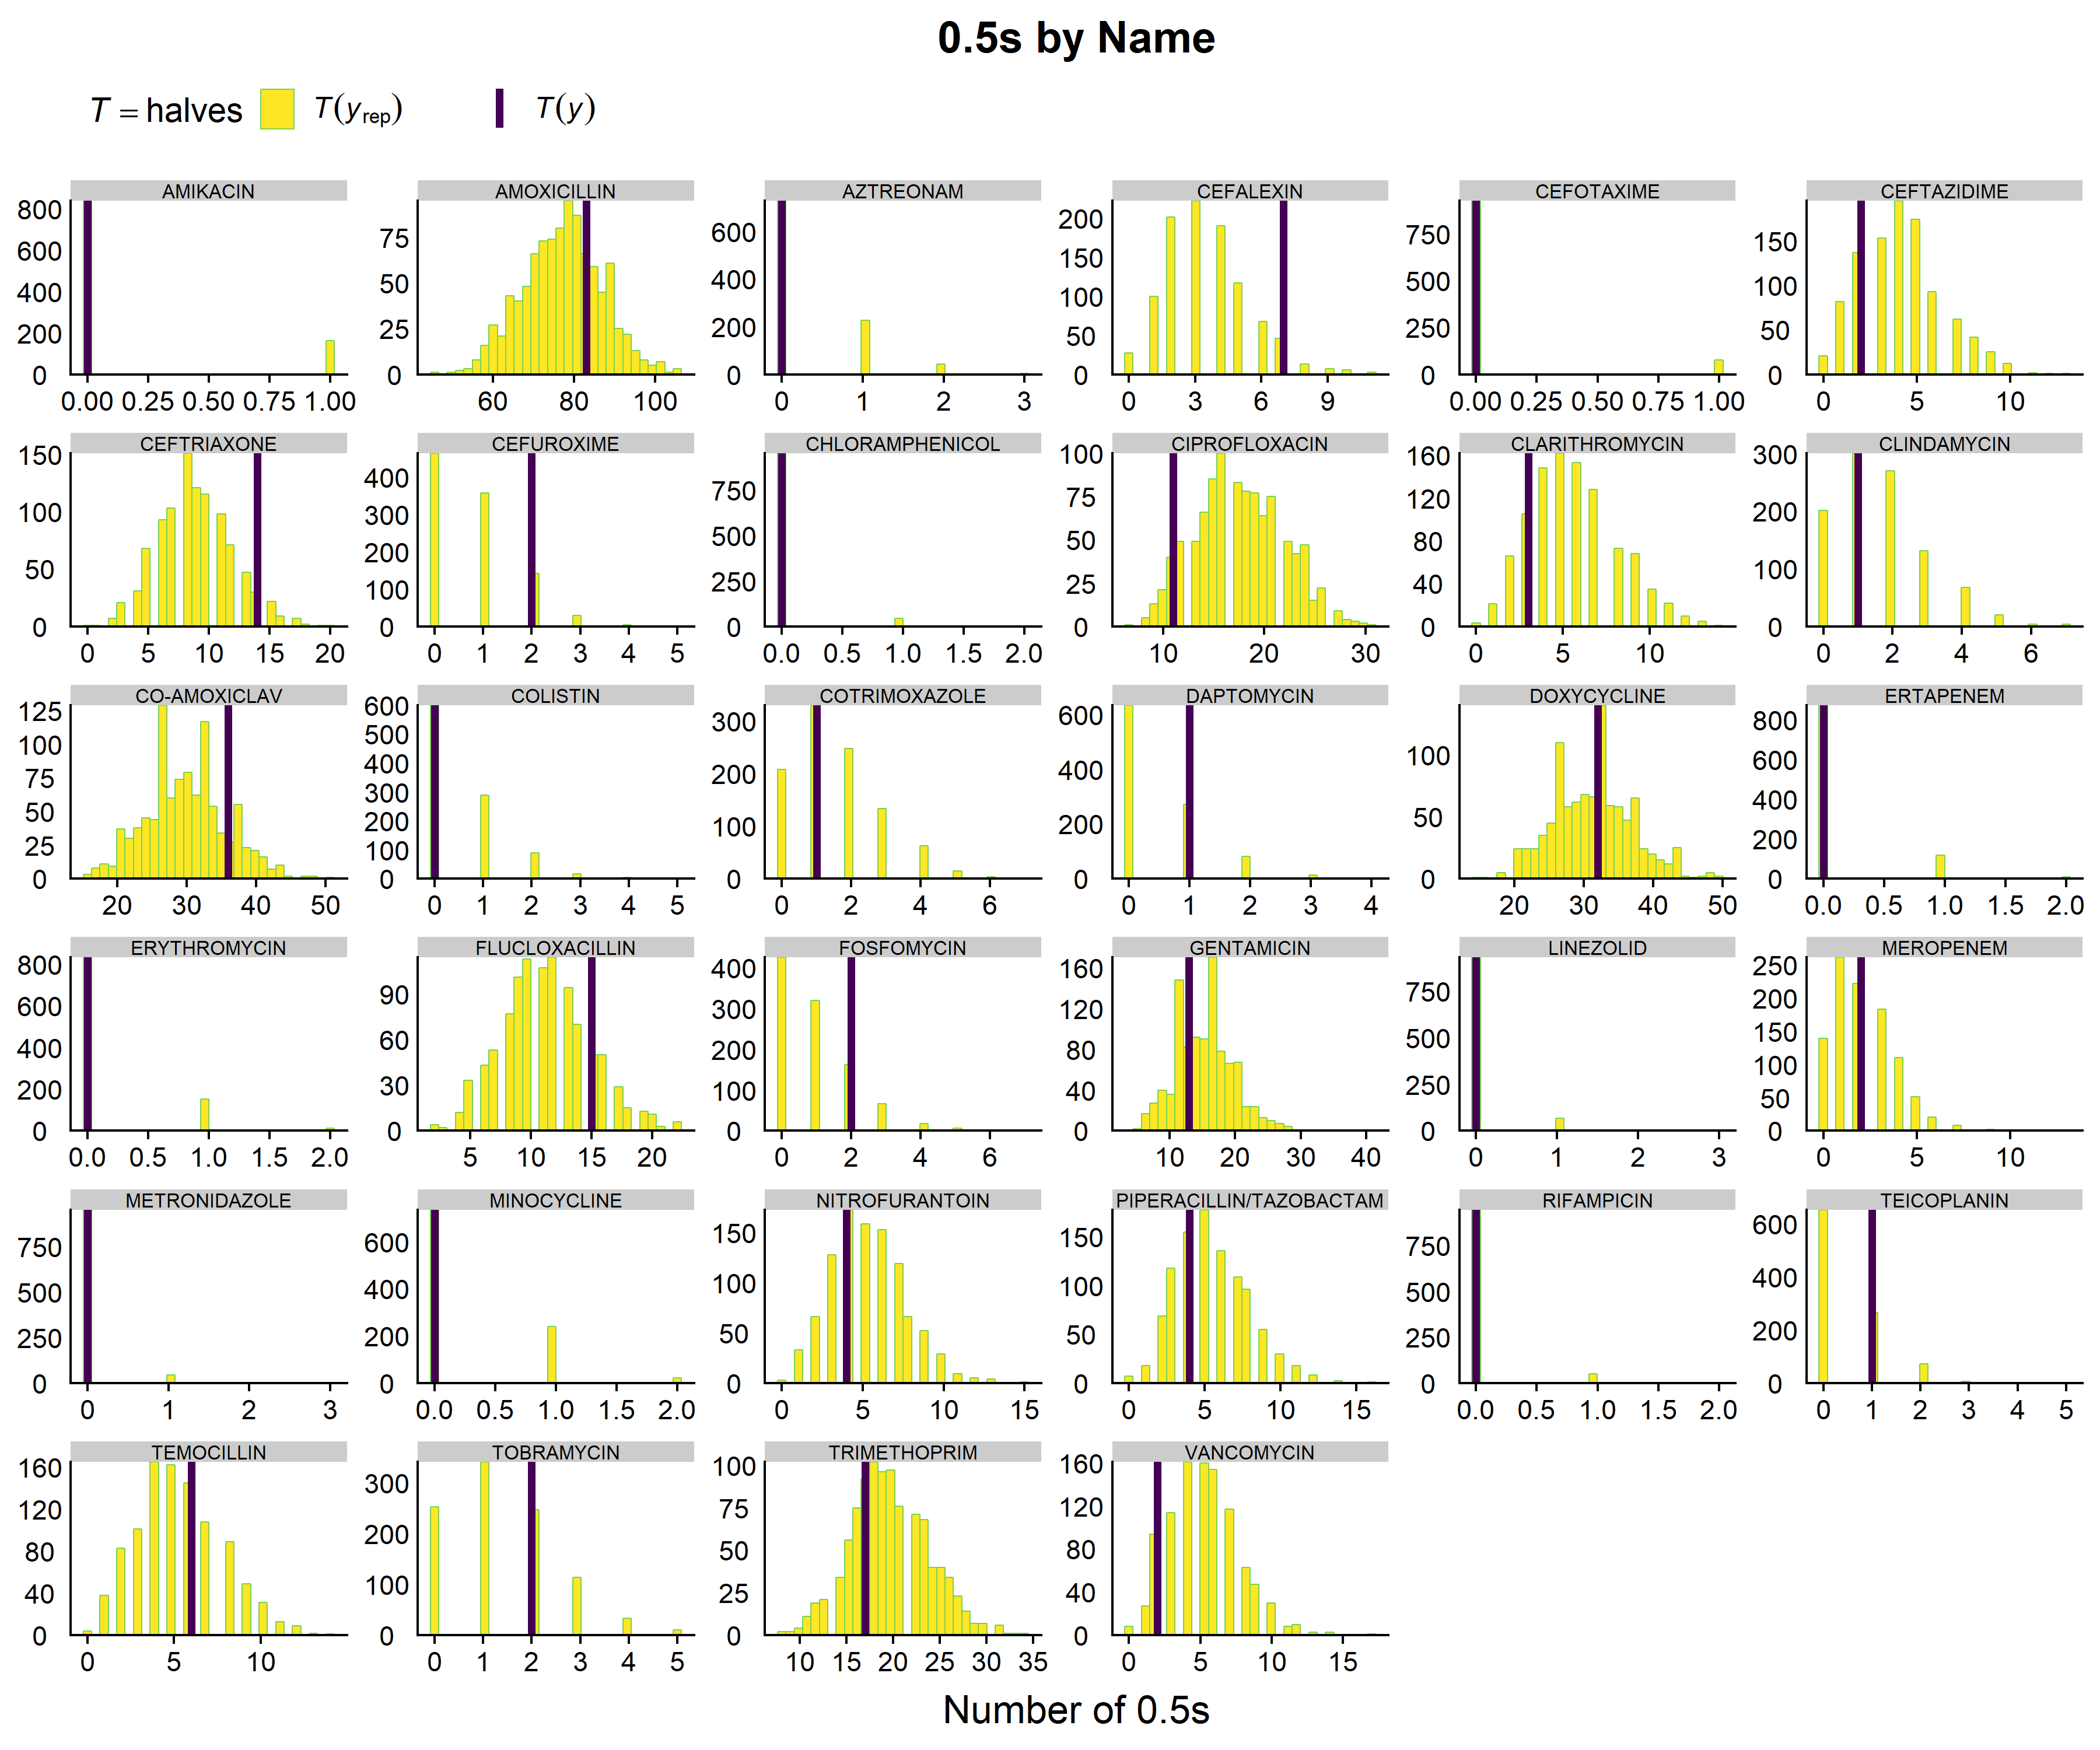
\includegraphics[width = 1\textwidth, height=0.45\textheight]{Figures/4_MC41_Halves.png}
	\caption{Test Statistic by Name (Number of 0.5s)} \label{fig::4_MC41_Halves}	
\end{figure}

\newpage

\begin{figure}[h!]
	\centering
	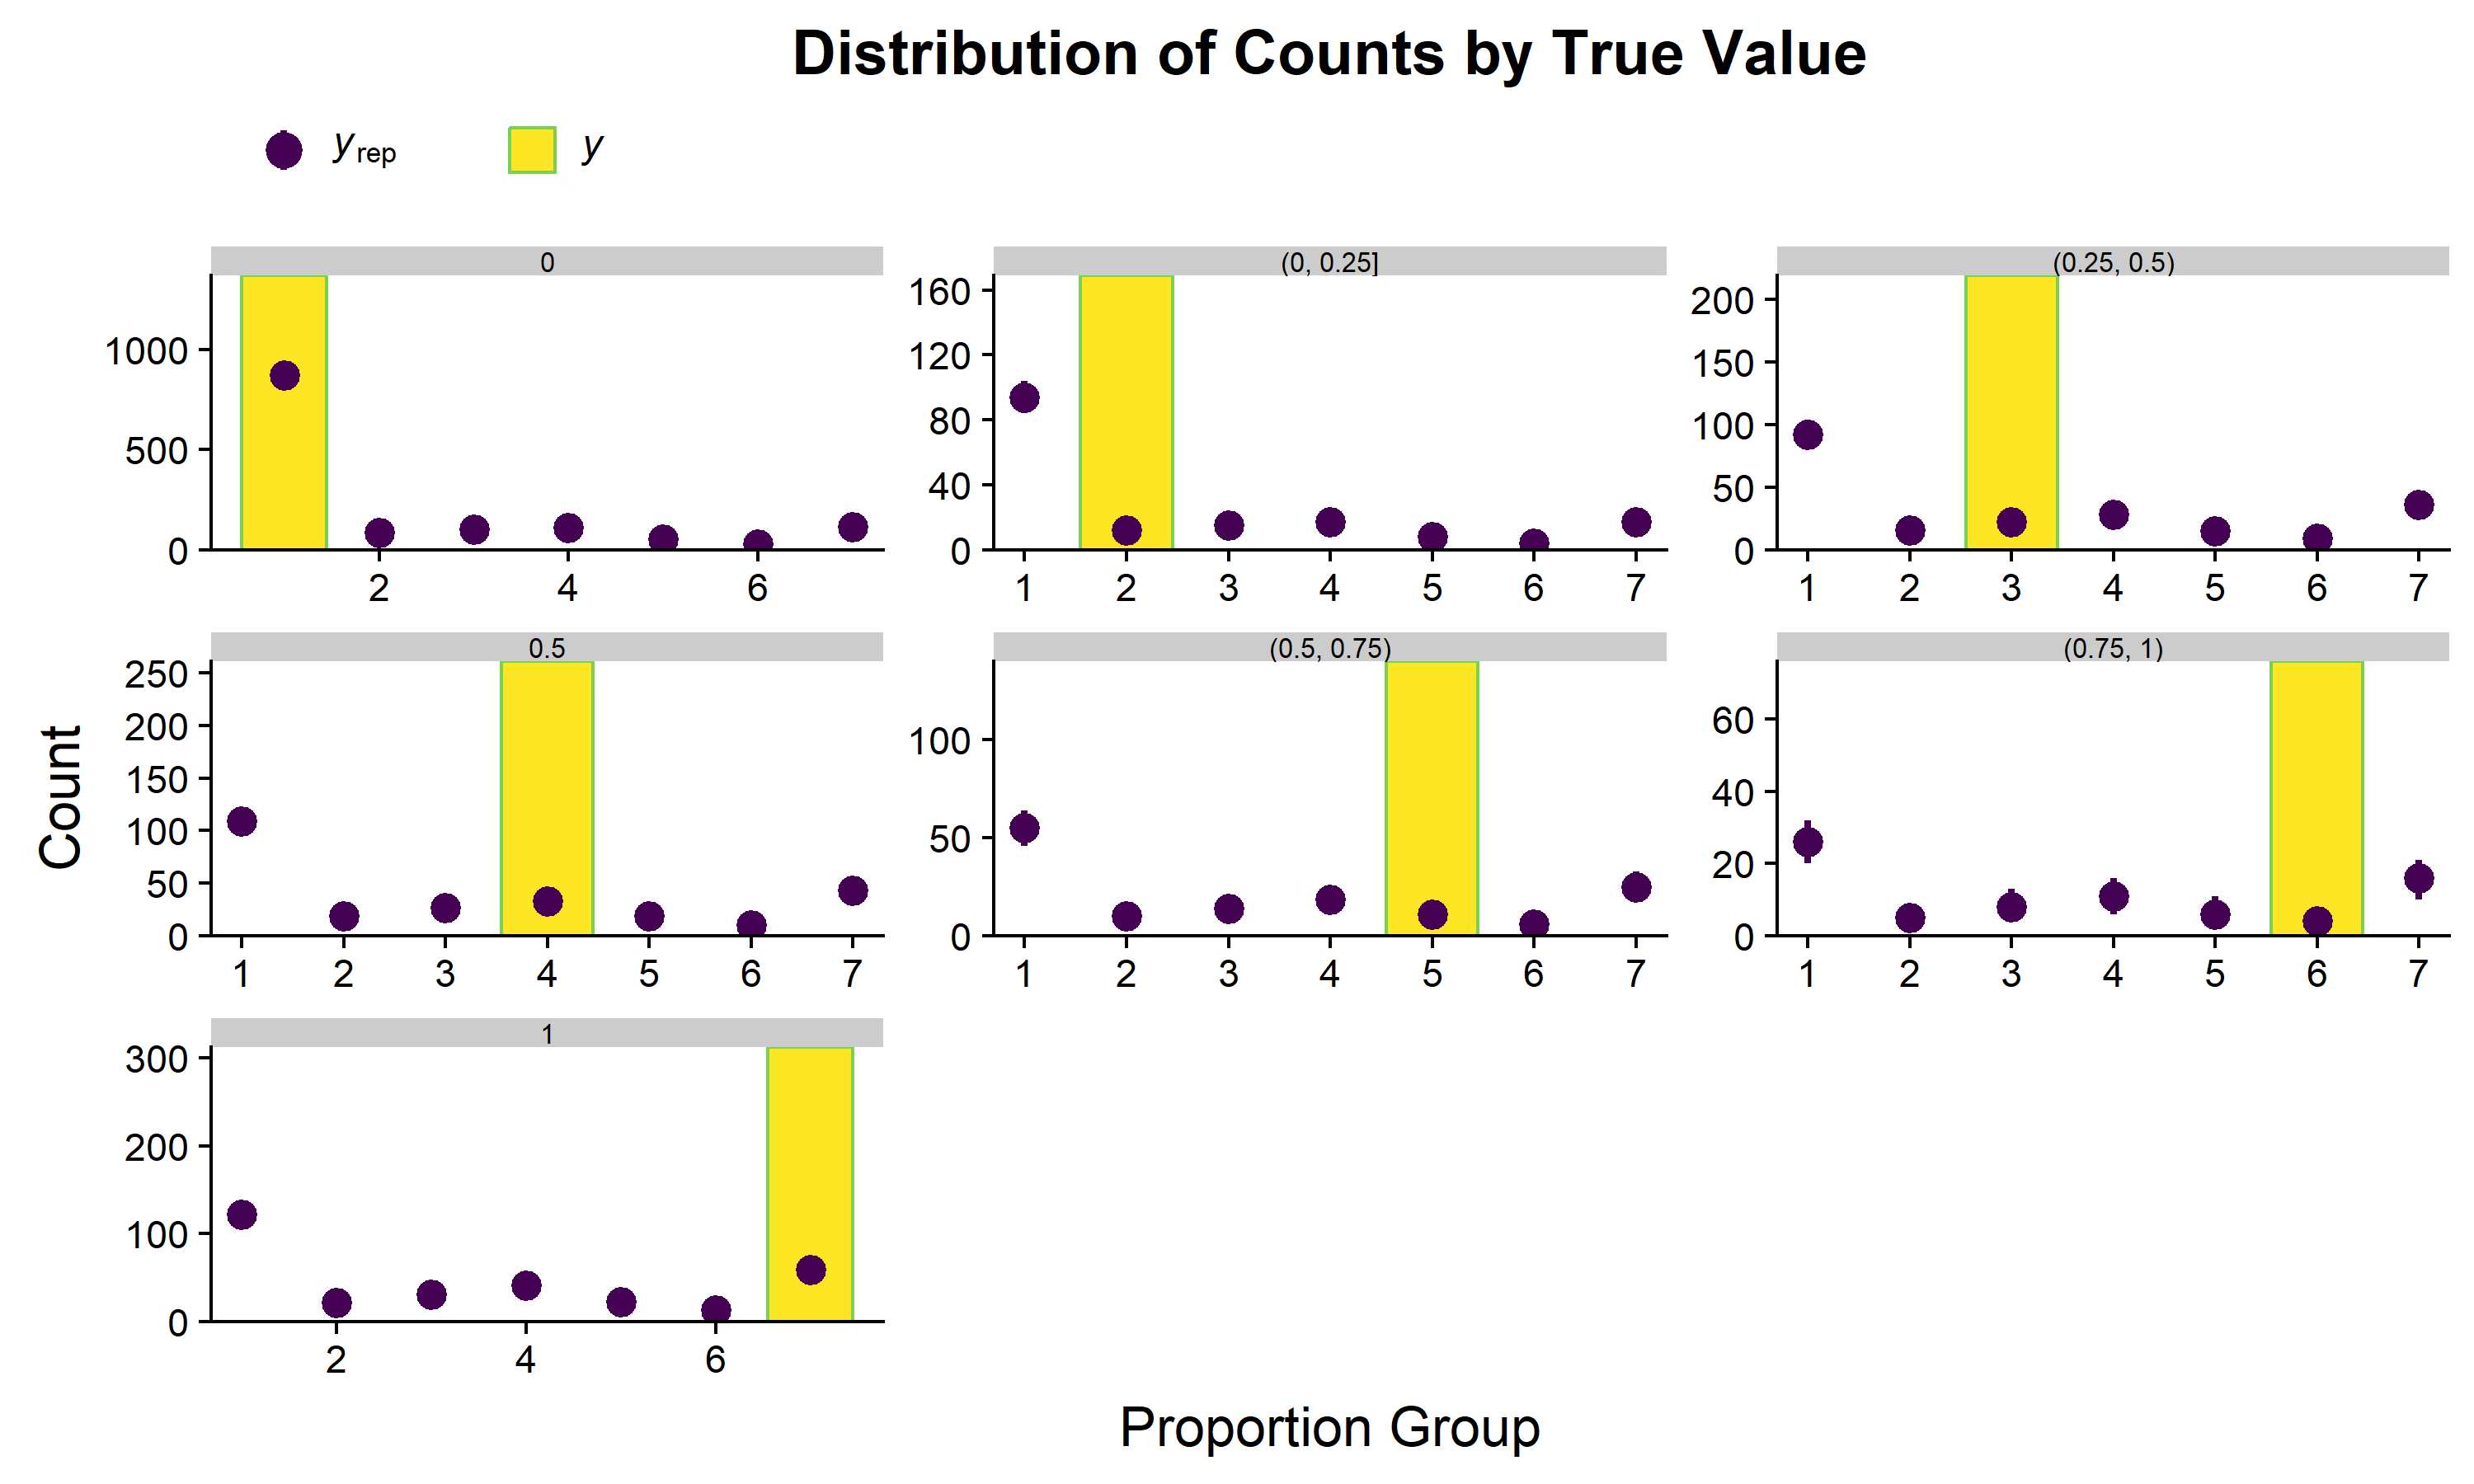
\includegraphics[width = \textwidth, height = 0.45\textheight]{Figures/4_MC41_BarPred.png}
	\caption{Predictions vs Truth} \label{fig::4_MC41_BarPred}	
\end{figure}


\begin{figure}[h!]
	\centering
	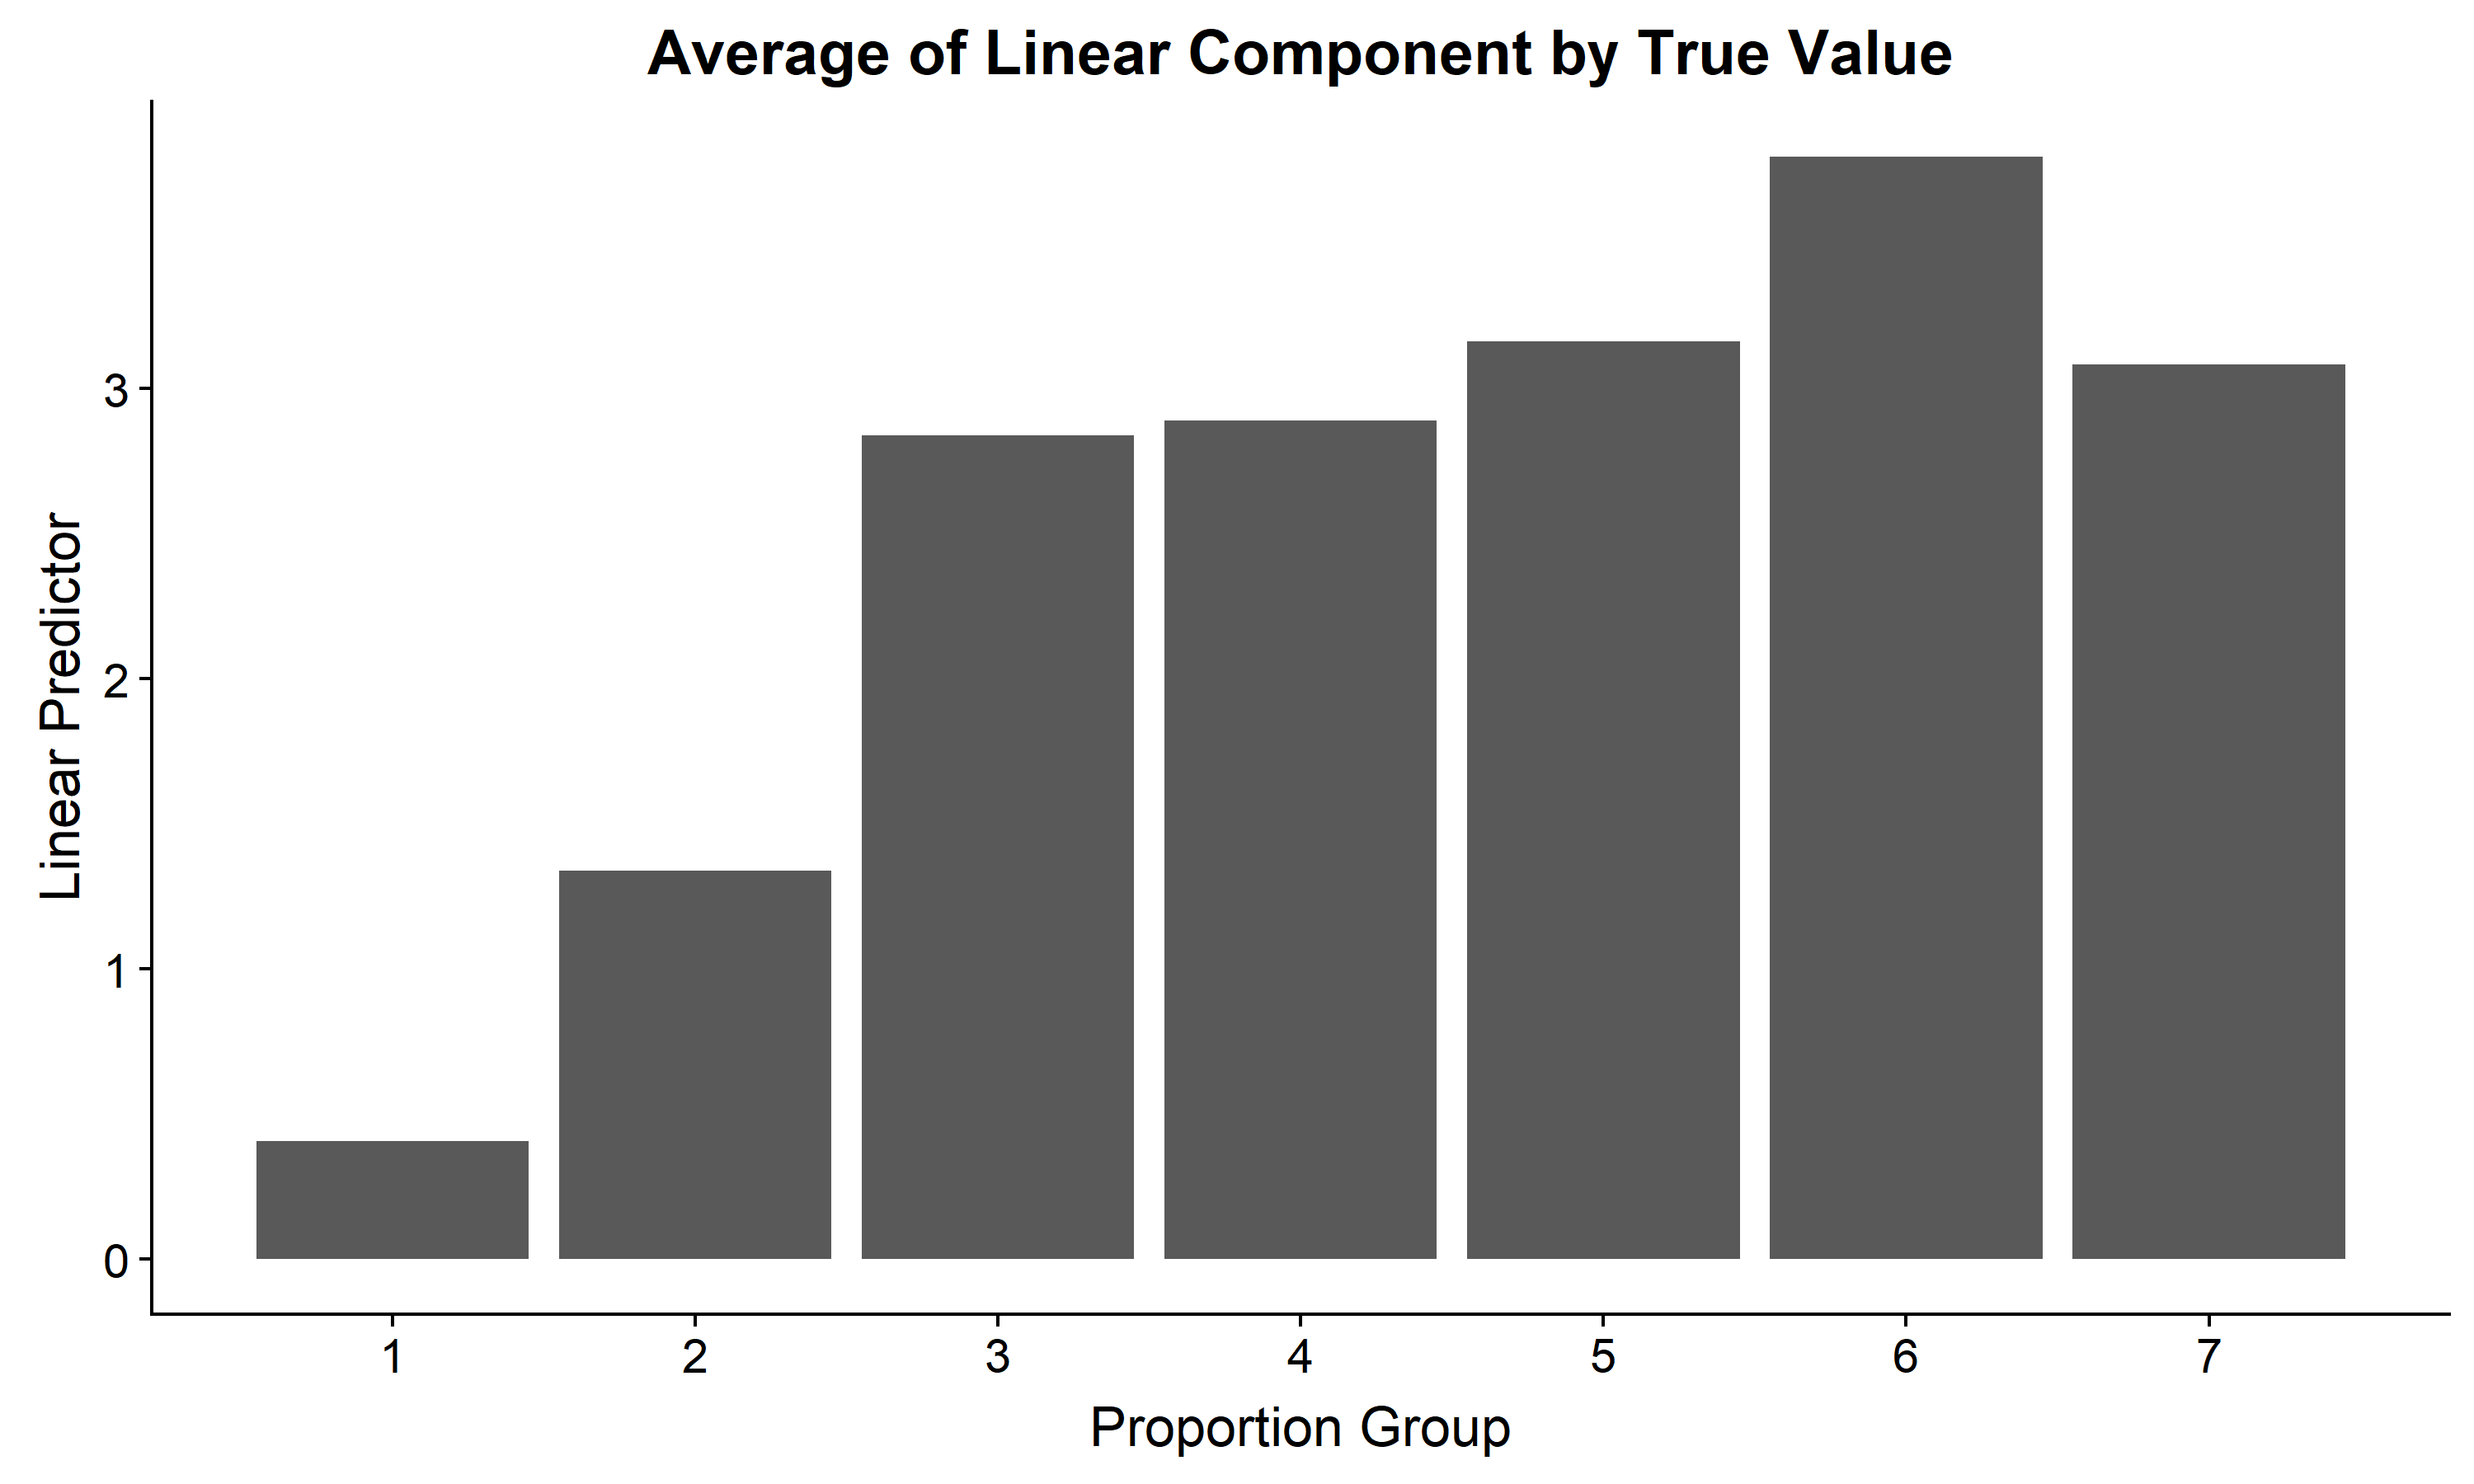
\includegraphics[width = \textwidth, height=0.43\textheight]{Figures/4_MC41_LinPred.png}
	\caption{Linear Predictor Value by True Value} \label{fig::4_MC41_LinPred}	
\end{figure}

\newpage

\clearpage





\newpage

\section{Results} \label{sec::Results}

\subsection{DDD and AMR}

The results for the population-level effects are in Table \ref{tab::5_Results_DDD}. The distributions for the key coefficients (i.e. involving DDD and route) are shown in Figure \ref{fig::5_Areas_DDD}. Under our model, there is a 95\% probability of a positive association between resistance and the DDD for invasively administered drugs. Specifically, we estimate a unit increase in the log DDD for invasive treatments increases the log-odds of a higher proportion group by 0.24.

It may be more intuitive to look at the latent scale, where Table \ref{tab::5_Transition_DDD} will assist us. We are still looking at \textit{invasively administered} drugs. Looking at the 2nd column, we can say a unit increase in the log DDD closes the distance between the first and second threshold by 26\%. Inverting this number, we see that to transition the whole gap, the log DDD needs to increase by 3.81. From this, we can calculate transition ratios -- the multiplier needed on raw DDD to push the linear predictor from the bottom of one group to the bottom of the next group up. This is the exponent of the values in the \texttt{Difference/$\beta_{lDDD}$} column. For example, to transition from the bottom of group 2 to the bottom of group 3 given a specific value of DDD $x_1$, the difference $x_2 - x_1$ needs to be such that $\frac{x_2}{x_1}$ is 45.\footnote{$log(x_2) - log(x_1) = 3.81 \iff \frac{x_2}{x_1} = exp(3.81) \approx 45$} This suggests that although the effect of DDD on resistance is likely positive, it is not overly important materially -- particularly considering the middle transition ratios. Recalling Figure \ref{fig::2_1_EDA_Cont} -- we can see that there is a low proportion of the higher values of raw DDD. The proportion of DDD values larger than 400 is only 6\%, suggesting that DDD changes are unlikely to be able to discriminate between groups, since such large values are so rare. 

However, it appears that transitioning from group 6 to 7 is more strongly determined by DDD (relatively), with a multiplicative effect of 24 for a bottom-to-bottom transition. In general, the \textit{importance} of DDD in group transitions appears to be higher at more extreme proportions, in terms of the ability to change the proportion group. We might hypothesise that there is some medical tipping-point phenomenon near the more extreme proportions, however this would require more domain expertise. 

\begin{table}[h!]
	\centering
	\begin{tabular}{lllllllll}
		\hline
		Parameter & Mean & SD & 2.5\% & 5\% & 95\% & 97.5\% & Pr($>$0) & Pr($<$0) \\ 
		\hline \hline
		$c_1$ & 1.94 & 0.81 & 0.42 & 0.66 & 3.30 & 3.58 & 0.99 & 0.01 \\ 
		$c_2$ & 2.85 & 0.85 & 1.32 & 1.55 & 4.33 & 4.64 & 1.00 & 0.00 \\ 
		$c_3$ & 4.11 & 0.96 & 2.45 & 2.66 & 5.79 & 6.18 & 1.00 & 0.00 \\ 
		$c_4$ & 5.82 & 1.17 & 3.76 & 4.05 & 7.86 & 8.35 & 1.00 & 0.00 \\ 
		$c_5$ & 6.96 & 1.34 & 4.60 & 4.93 & 9.32 & 9.88 & 1.00 & 0.00 \\ 
		$c_6$ & 7.72 & 1.46 & 5.14 & 5.50 & 10.28 & 10.89 & 1.00 & 0.00 \\ 
		$\beta_{Age}$ & 0.14 & 0.11 & -0.07 & -0.03 & 0.32 & 0.37 & 0.90 & 0.10 \\ 
		$\beta_{lDDD}$ & 0.24 & 0.15 & -0.04 & 0.00 & 0.51 & 0.57 & 0.95 & 0.05 \\ 
		$\beta_{NonInvasive}$ & 1.75 & 0.97 & -0.01 & 0.25 & 3.45 & 3.84 & 0.97 & 0.03 \\ 
		$\beta_{lDDD*NonInvasive}$ & -0.36 & 0.21 & -0.81 & -0.72 & -0.04 & 0.02 & 0.03 & 0.97 \\ 
		$\beta_{lDDD} + \beta_{lDDD*NonInvasive}$ & -0.12 & 0.15 & -0.42 & -0.37 & 0.12 & 0.17 & 0.20 & 0.80 \\ 
		\hline
		\hline
	\end{tabular}
	\caption{Results Table (Population Effects)} 
	\label{tab::5_Results_DDD}
\end{table}


\begin{table}[h!]
	\centering
	\begin{tabular}{lllll}
		\hline
		& Difference & $\beta_{lDDD}$/Difference & Difference/$\beta_{lDDD}$ & Transition Ratios \\ 
		\hline \hline
		$c_2 - c_1$ & 0.91 & 0.26 & 3.81 & 45.04 \\ 
		$c_3 - c_2$ & 1.26 & 0.19 & 5.27 & 193.99 \\ 
		$c_4 - c_3$ & 1.71 & 0.14 & 7.15 & 1269.58 \\ 
		$c_5 - c_4$ & 1.15 & 0.21 & 4.79 & 120.90 \\ 
		$c_6 - c_5$ & 0.76 & 0.32 & 3.16 & 23.65 \\ 
		\hline
	\end{tabular}
	\caption{Group Transition Table} 
	\label{tab::5_Transition_DDD}
\end{table}

\newpage

For \textit{non-invasive} administration, there is a 97\% probability the association between DDD and proportion is smaller than for \textit{invasive} administration ($\beta_{lDDD*NonInvasive}$). The \textit{overall} ceteris paribus\footnote{All else being equal} effect of an increase in log DDD for a non-invasively administered drug is, on average, a reduction of 0.12 on the latent scale, with an 80\% probability the association is negative, hence a 20\% probability it is positive. Therefore, there is lots of uncertainty around the association of DDD for non-invasive drugs, so we should not commit to any conclusions.\\

Summarising, we can note that the association between DDD and the proportion:


\begin{enumerate}
	\item Is positive for invasively administered drugs (95\%, $\beta_{lDDD}$)
	\item Is smaller for non-invasively administered drugs (97\%, $\beta_{lDDD*NonInvasive}$)
	\item \textit{May} be negative for non-invasive drugs (80\%, $\beta_{lDDD} + \beta_{lDDD*NonInvasive}$)
\end{enumerate}


\begin{figure}[h!]
	\centering
	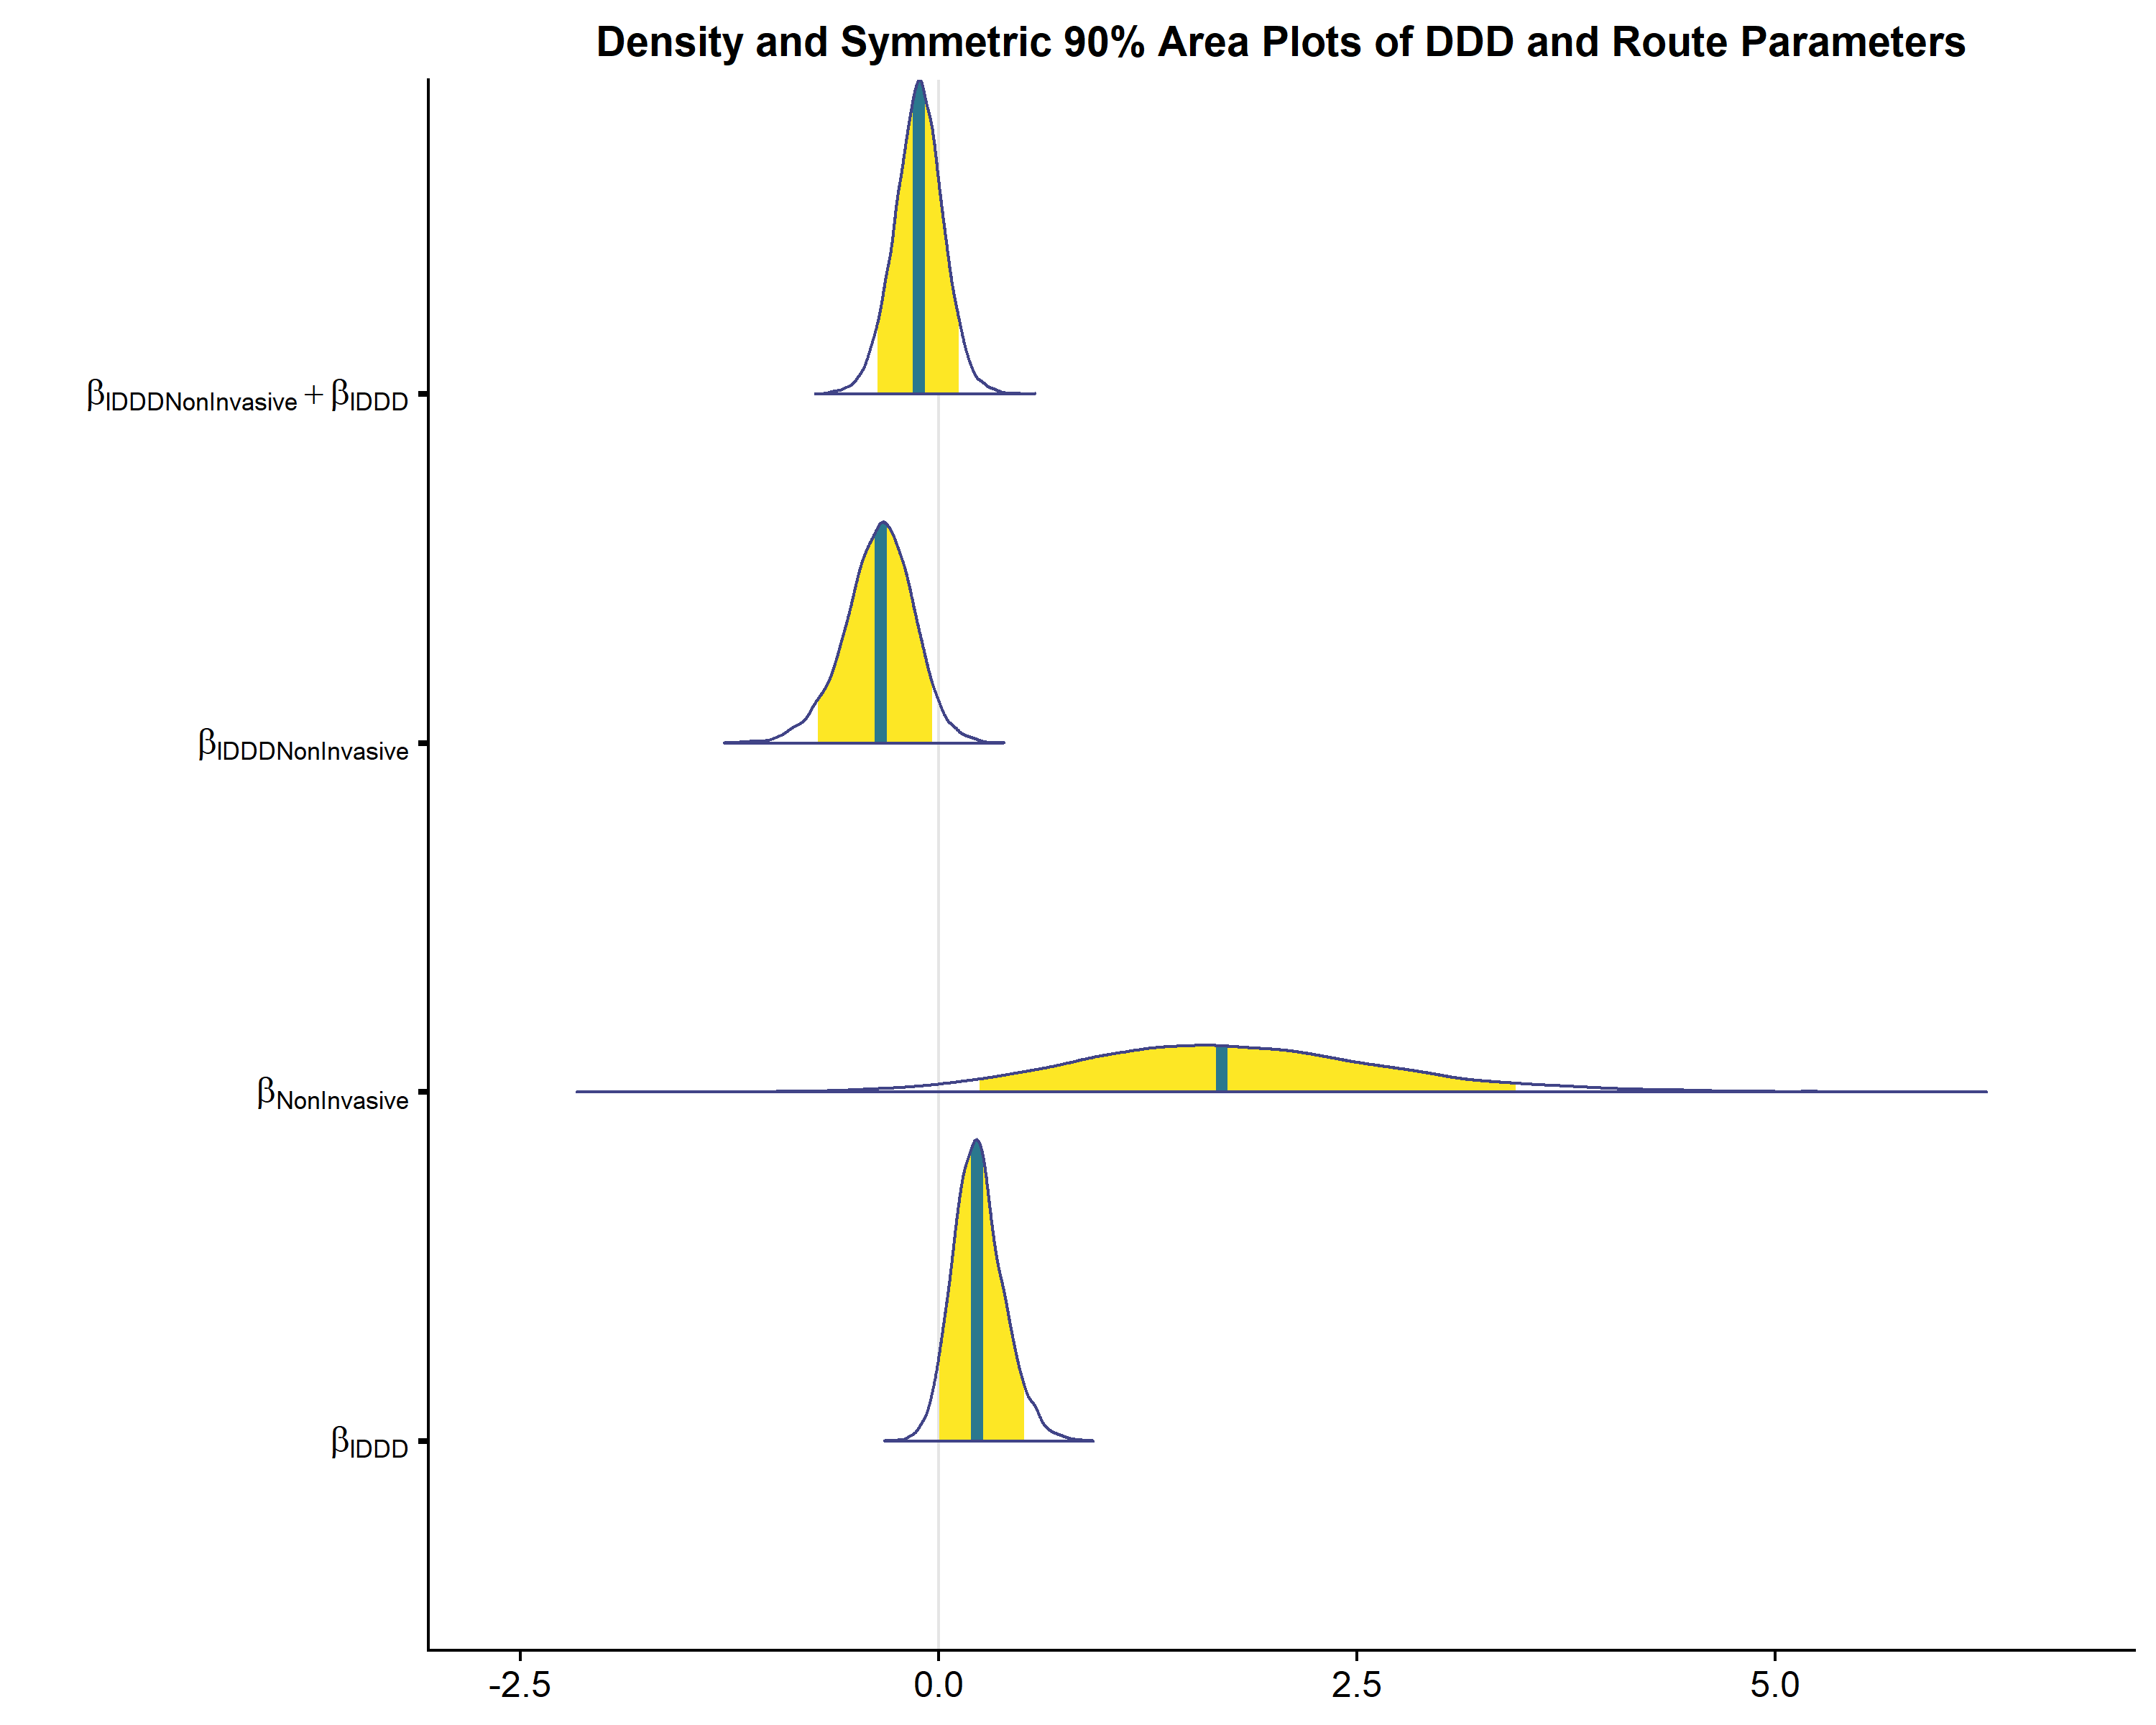
\includegraphics[width = 1\textwidth]{Figures/5_1_Areas_DDD.png}
	\caption{Posterior Area Plots (DDD and Route)} \label{fig::5_Areas_DDD}	
\end{figure}

\subsubsection{Route}

Ceteris paribus, non-invasive administration has a much higher chance of falling into a higher bin, with a mean of 1.75, and a 97\% probability of non-invasive administration being associated with higher proportions. Reviewing the thresholds, it appears that the administration route being non-invasive is enough, on average, to achieve a bottom to bottom transition for each group -- suggesting it is an important predictor of AMR. 


\newpage

\subsection{Drug-Specific Effects}

Posterior interval plots of the varying intercepts are shown in Figure \ref{fig::5_Intervals_Name}, with lines at -3 and 3. It appears a large part of the hospital resistance is being driven by a few drugs, with only 5 drugs having 90\% symmetric credible intervals not containing 0. The highest magnitudes come from amoxicillin, doxycycline, and trimethoprim (minocycline is excluded due to its wide intervals). On the other side, linezolid, meropenem, and metronidazole all have a strong negative relationship with resistance.  

\begin{figure}[h!]
	\centering
	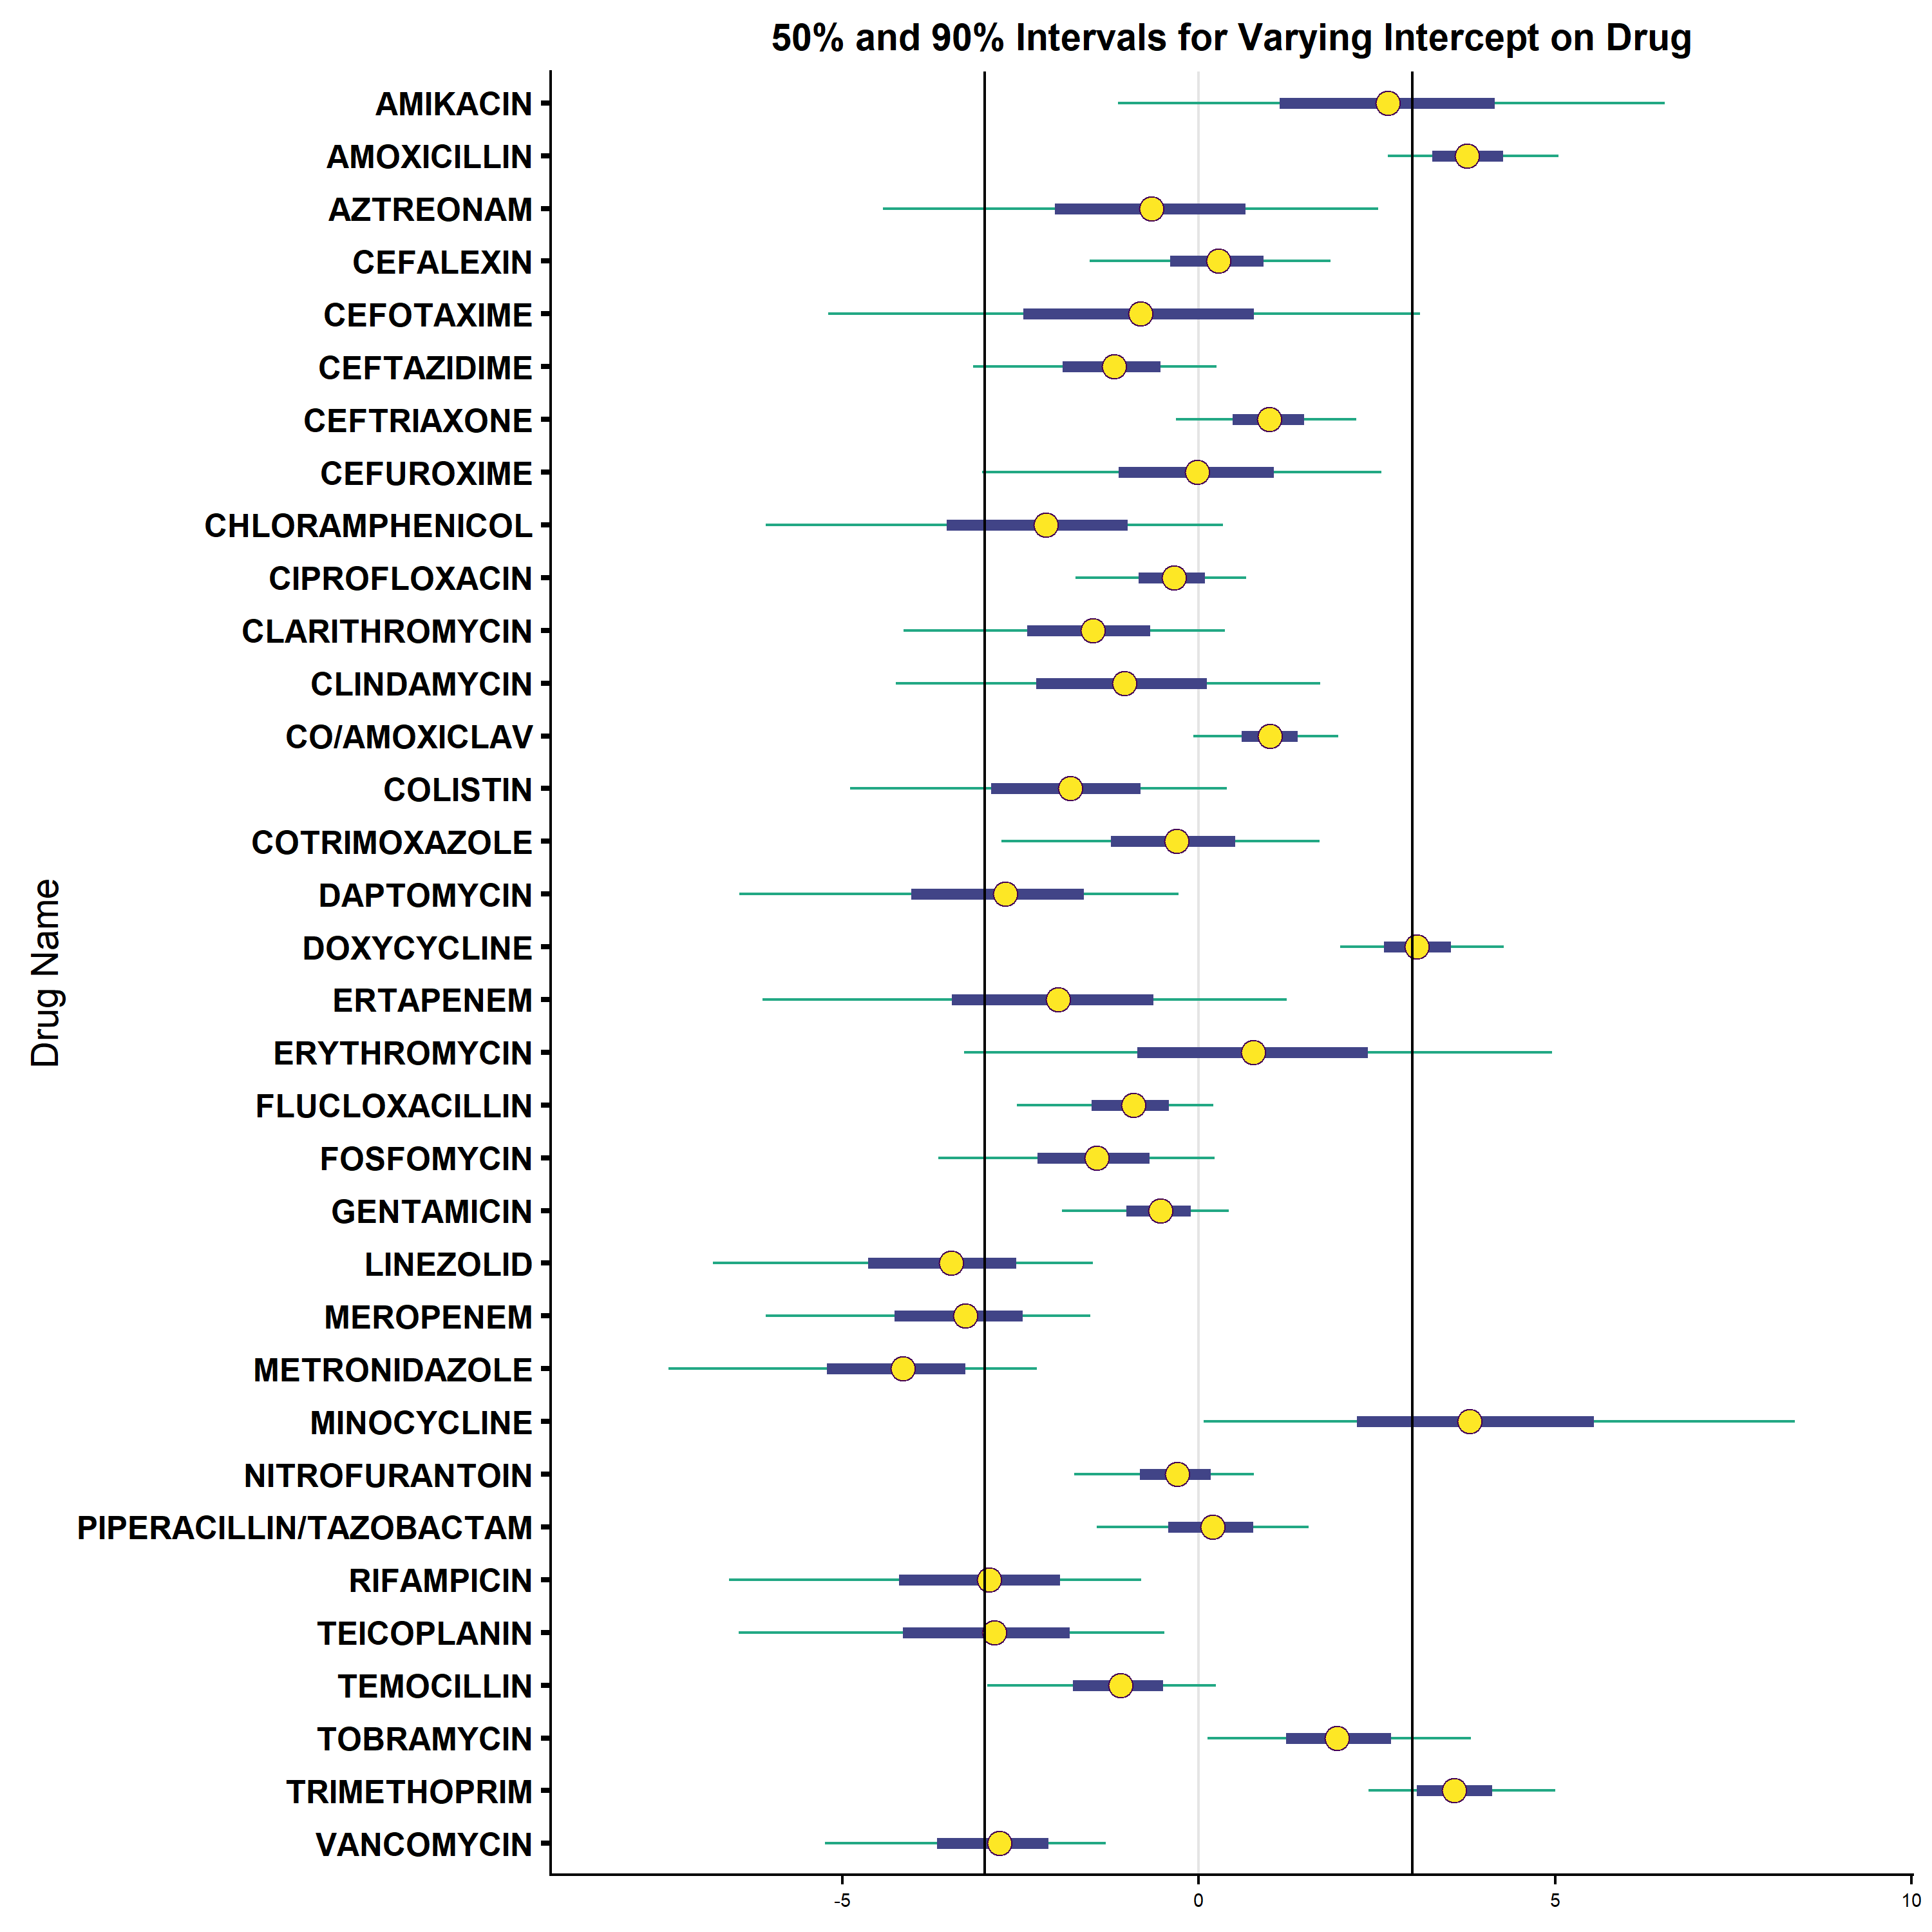
\includegraphics[width = 1\textwidth]{Figures/5_1_Intervals_Name.png}
	\caption{Posterior Interval Plots (Drug Name)} \label{fig::5_Intervals_Name}	
\end{figure}

\newpage
\subsection{Class Group Heterogeneity}

We transform the discrimination parameter to the standard deviation\footnote{By transforming each individual sample using s = 1/exp(log(disc))). The output of \texttt{brms} already contains the discrimination on the log scale.} for interpretation. $\sigma_j$ refers to the standard deviation of class group $j$, relative to group A. 

All groups are more variable than group A (as expected, since there was no resistance in A), and most variability (relative to A) is between 2 and 3. However, E shows much more variability in the latent variable, with the lower bound of its 95\% credible interval being 3.53. That is 3.5 times higher than the standard deviation of the group A, and almost twice as variable as group C. 

\begin{table}[h!]
	\centering
	\begin{tabular}{lllll}
		\hline
		& Mean & SD & 2.5\% & 97.5\% \\ 
		\hline \hline
		$\sigma_B$ & 2.28 & 0.55 & 1.42 & 3.52 \\ 
		$\sigma_C$ & 1.84 & 0.40 & 1.18 & 2.71 \\ 
		$\sigma_D$ & 2.90 & 0.59 & 1.91 & 4.19 \\ 
		$\sigma_E$ & 6.01 & 1.56 & 3.53 & 9.70 \\ 
		$\sigma_F$ & 2.65 & 0.53 & 1.76 & 3.82 \\ 
		$\sigma_G$ & 2.50 & 0.51 & 1.63 & 3.64 \\ 
		\hline
	\end{tabular}
	\caption{Class Group Heterogeneity} 
	\label{tab::5_Heterogeneity}
\end{table}

\subsection{Comments on Other Fitted Models}

Our hypothesised model (\texttt{mp1}), and the model with a class-varying intercept (\texttt{mc31}) both also had probabilities of the log DDD parameter being positive for invasive administration, this time with above 99\% probability. For models with log DDD as a population effect, the minimum probability of a positive relationship was 71\% (excluding the overfit model due to the lack of theoretical properties, and the varying slopes models due to no concise measure).

\vspace*{3mm}

Varying slopes were found to have near-zero standard deviations on all group-level slopes, and wide intervals for the correlations - suggesting there is not enough\footnote{``Not enough" refers to data \textit{quality}, not the number of observations. It can be thought of as saying the data does not contain strong evidence} data to determine correlations between the varying intercepts and slopes. For example \texttt{mc32} suggests only a 75\% probability the standard deviation between the varying slopes of log DDD was greater than 0.05. The smallest width of a 95\% credible interval for estimated correlations was 1.56 -- 78\% of the whole range of values. Furthermore, the highest probability a correlation was more or less than 0 was only 68\%. The combination of the small standard deviation estimates, and the wide intervals for correlations suggest a group-level slope is a needless complication given our limited data. 

\newpage
\section{Model Discussion} \label{sec::Discussion}

\subsection{Concerns}

As noted, the predictive performance of the model was poor, mostly due to the high variability in the data, the limited covariates, and the small data (2548 rows). Additionally, though the latent variable should be higher with each group, there was a dip from group 6 to group 7. 

Furthermore, we should be sceptical of generalising results from this data as it is based solely on the WGH. There may be location-specific effects, or hospital-specific effects that we cannot pick up on due to examining a niche subset of the population. 

A weakness of the cumulative logit is that it assumes a unit increase in the covariates has the same impact on the log-odds regardless of the group in question. Alternative methods that can account for so-called category-specific effects are the sequential model, and the adjacent category model (\citeauthor{BurknerVuorre2018}, \citeyear{BurknerVuorre2018}). However the theoretical intuition is not cohesive with our problem structure, with the adjacent category model in particular being difficult to interpret. 

\subsection{Alternative Model: Zero-one inflated Beta (ZOIB)}

Previously, a ZOIB (\citeauthor{Ospina2008}, \citeyear{Ospina2008}) model was fitted to the data, however even posterior histograms and density plots fit the data relatively poorly, specifically the intermediate proportions. In addition, the complexity of interpretation due to the separate logistic models internally fitted meant the model was an unattractive proposition, despite the raw proportion seemingly following such a distribution. \\

Though not implemented due to time constraints, it may be of interest to combine the ordered logit with the ZOIB, by recalling section \ref{sec::3_Latent}. We can attempt to determine whether the latent variable implies a 0, a 1, or if it passes through the function $g$. In the latter case, we could use a beta regression, as all responses constructed by $g$ are in (0,1). Currently, ZOIB ignores the ordering of data, and models the 0s and 1s as a separate process. This contributes to its difficult interpretation. For instance, a parameter suggesting an increase in a covariate $x$ is associated with the response $y$ being in \{0,1\} cannot be interpreted directly, since we cannot see the directional effect (i.e. lower or higher values of $y$) of a covariate, because 0 and 1 are opposed. As such, this covariate must be interpreted in multiple equations, and its parameters do not have a clean form suggesting whether its overall impact is positive or negative. \\

Another approach to finding the contribution to the overall mean is marginalisation of the ZOIB. Marginalisation of a two-part model is discussed in \cite{SmithMarginalised}, but the concepts should extend to ZOIB. 

\newpage

\section{Conclusion} \label{sec::Conclusion}

The objective of this paper was to establish if there exists an association between drug use (measured in DDD/1000 OBD) and AMR (measured by proportion of clinical isolates exhibiting resistance) at the hospital level, using a Bayesian orderd logit model. \\

We find a 95\% probability of a positive association between DDD and AMR for invasively administered drugs, with a 97\% probability that non-invasive administration leads to a smaller association between DDD and AMR. This latter association may even be negative, however the probability of this is only 80\% which is too small to draw conclusions from. The relative importance of invasively administered DDD in determining the proportion group is small, with a minimum transition ratio of 23.65 for a bottom to bottom transition. These ratios were smallest at more extreme proportions, perhaps implying a tipping-point phenomenon.  \\

In general, resistance mostly arises from a few drugs - namely amoxicillin, doxycycline, and trimethoprim. The drugs with the most negative association were linzolid, meropenem, and metronidazole. 

We have also suggested an alternative model (ZOIB), and how it might be improved by accounting for the natural ordering in the data, which is currently ignored. Marginalisation is also an attractive proposition. 

Concerns involve the generalisability of the model due to the subpopulation of a single hospital which could mean ignored hospital-specific or location-specific effects. The average age of patients is also very high, with the minimum average age on a ward-week being 45. Additionally, there may be selection bias due to the study being in a hospital setting where people are already ill. There is also the concern of the model's poor predictive performance, even when considering the purposefully overfit model.  





\clearpage

% the entries have to be in the file literature.bib
\bibliographystyle{agsm}
\bibliography{Bibliography}
\clearpage

\appendix
\section*{Appendices}
\addcontentsline{toc}{section}{Appendices}

\section{Data Preparation}

Figure \ref{fig::Missingness} shows that around 36\% of the data was missing, primarily in the resistance proportion. All data was dropped. For the covariates, the little data missing is insignificant. For the resistance proportion, the data was missing in the sense that it was never measured, \textbf{not} because there was some mechanism that caused values to not be reported. This is because the clinical isolates were not relevant to the drug. 

We grouped the route into ``Invasive" and ``Non-Invasive" groups, due to limited observations for rectal transmission. Additionally, we removed a row which had a DDD of 0 due to irrelevance.

\begin{figure}[h]
    \centering
    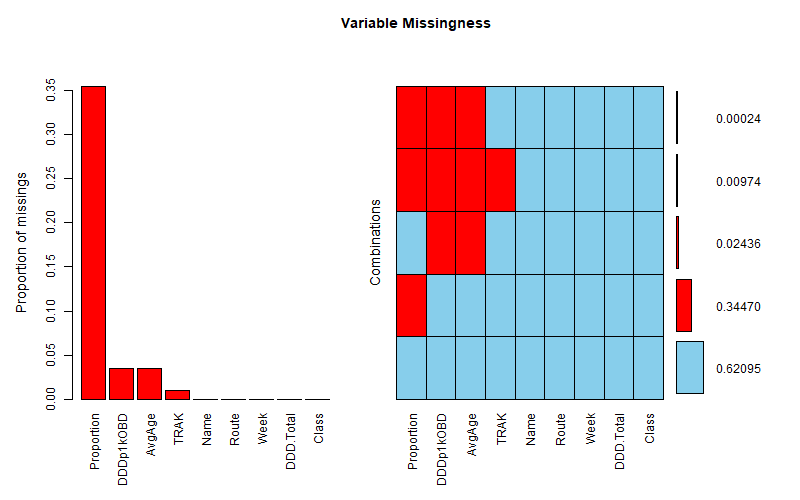
\includegraphics[width = 0.7\textwidth, height=0.25\textheight]{Figures/1_Missing.png}
    \caption{Missingness} \label{fig::Missingness}
\end{figure}

Figure \ref{fig::Missingness} was created using the \texttt{VIM} package by \cite{VIM}. 

\newpage

\section{Models Compared}
\label{app:ModelSpec}

This section outlines all of the models compared in this report. brms syntax was used to keep things concise, and we shortened the formula further using individual letters. The corresponding terms are in the first table. All models used 3 chains. Runtimes varied between 10 and 30 minutes for all models except the overfit model - which took over 1 hour. The machine was a Dell Inspiron 15-7559, running Windows 10 Home 64-bit, an Intel(R) Core(TM) i5-6300 HQ CPU @ 2.30 GHz, with 4 cores. Note that chains were run on separate cores. 

Expressions included prior to $|$ within brackets are group-level effects, while those outside are constant. \texttt{adapt\_delta} is a parameter controlling the step size of the HMC algorithm. The maximum value is 1, and higher values make for slower computation, but help to avoid divergent transitions. 


\begin{table}[h!]
	\centering
	\begin{tabular}{|l|l|}
		\hline
		Letter & Stands For \\ \hline
		A & Average age (standardised) \\
		C & Class\\
	    CG & Grouped Class \\
		D & log DDD per 1000 OBD \\
		N & Drug name \\
		P & Grouped Proportion \\
		R & Route \\ \hline
	\end{tabular} \caption{Drug Class Groupings}\label{table::acronyms}
\end{table}

\begin{table}[h!]
	\centering
	\begin{tabular}{|l|l|l|l|l|}
		\hline
		Name & brms formula & warmup & iterations & adapt\_delta \\ \hline 
		mp1 & \texttt{P $\sim$ A + D*R + (1$|$CG)} & 2500 & 6000 & 0.9 \\
		mc1 & \texttt{P $\sim$ A + D*R*N} & 1000 & 4000 & 0.9 \\ 
		mc2 & \texttt{P $\sim$ (1 + A + D*R$|$N)} & 1000 & 4500 & 0.98 \\
		mc31 & \texttt{P $\sim$ A + D*R + (1$|$C)} & 1000 & 4500 & 0.91 \\
		mc32 & \texttt{P $\sim$ A + (1+D*R$|$C)} & 2000 & 5000 & 0.99 \\
		mc33 & \texttt{P $\sim$ A + R + (1+D$|$C)} & 2000 & 5000 & 0.95 \\
		mc34 & \texttt{P $\sim$ A + R + D + (1$|$C)} & 2000 & 5000 & 0.9 \\
		mc41 & \texttt{P $\sim$ A + (1+D*R$|$N)} & 1000 & 4500 & 0.91 \\
		mc42 & \texttt{P $\sim$ A + D*R + (1$|$N)} & 1000 & 4500 & 0.95 \\
		mc43 & \texttt{P $\sim$ A + R + (1+D$|$N)} & 1000 & 4500 & 0.98 \\
		mc44 & \texttt{P $\sim$ A + R + D + (1$|$N)} & 1000 & 4500 & 0.9 \\ \hline
	\end{tabular} \caption{Drug Class Groupings}\label{table::appfullmod}
\end{table}


\clearpage

\section{R Session Information}
\label{app:two}

\begin{verbatim}
R version 3.5.3 (2019-03-11)
Platform: x86_64-w64-mingw32/x64 (64-bit)
Running under: Windows 10 x64 (build 17134)

Matrix products: default

locale:
[1] LC_COLLATE=English_United States.1252  LC_CTYPE=English_United States.1252   
[3] LC_MONETARY=English_United States.1252 LC_NUMERIC=C                          
[5] LC_TIME=English_United States.1252    

attached base packages:
[1] grid      stats     graphics  grDevices utils     datasets  methods   base     

other attached packages:
[1] xtable_1.8-4      brms_2.9.3        Rcpp_1.0.1        dplyr_0.8.1       VIM_4.8.0        
[6] colorspace_1.4-1  loo_2.1.0         bayesplot_1.7.0   data.table_1.12.2 cowplot_0.9.4    
[11] ggplot2_3.1.1    

loaded via a namespace (and not attached):
[1] class_7.3-15         rio_0.5.16           ggridges_0.5.1       rsconnect_0.8.13    
[5] markdown_0.9         base64enc_0.1-3      rstudioapi_0.10      rstan_2.18.2        
[9] audio_0.1-6          DT_0.6               mvtnorm_1.0-10       ranger_0.11.2       
[13] bridgesampling_0.6-0 robustbase_0.93-5    shinythemes_1.1.2    packrat_0.5.0       
[17] shiny_1.3.2          compiler_3.5.3       tictoc_1.0           backports_1.1.4     
[21] assertthat_0.2.1     Matrix_1.2-15        lazyeval_0.2.2       cli_1.1.0           
[25] later_0.8.0          beepr_1.3            htmltools_0.3.6      prettyunits_1.0.2   
[29] tools_3.5.3          igraph_1.2.4.1       coda_0.19-2          gtable_0.3.0        
[33] glue_1.3.1           reshape2_1.4.3       carData_3.0-2        cellranger_1.1.0    
[37] nlme_3.1-137         crosstalk_1.0.0      lmtest_0.9-37        laeken_0.5.0        
[41] stringr_1.4.0        ps_1.3.0             openxlsx_4.1.0       mime_0.6            
[45] miniUI_0.1.1.1       gtools_3.8.1         DEoptimR_1.0-8       MASS_7.3-51.1       
[49] zoo_1.8-5            scales_1.0.0         colourpicker_1.0     hms_0.4.2           
[53] promises_1.0.1       Brobdingnag_1.2-6    parallel_3.5.3       inline_0.3.15       
[57] shinystan_2.5.0      curl_3.3             gridExtra_2.3        StanHeaders_2.18.1  
[61] stringi_1.4.3        dygraphs_1.1.1.6     e1071_1.7-1          boot_1.3-20         
[65] pkgbuild_1.0.3       zip_2.0.2            rlang_0.3.4          pkgconfig_2.0.2     
[69] matrixStats_0.54.0   lattice_0.20-38      purrr_0.3.2          rstantools_1.5.1    
[73] htmlwidgets_1.3      labeling_0.3         tidyselect_0.2.5     processx_3.3.1      
[77] plyr_1.8.4           magrittr_1.5         R6_2.4.0             pillar_1.4.0        
[81] haven_2.1.0          foreign_0.8-71       withr_2.1.2          xts_0.11-2          
[85] abind_1.4-5          sp_1.3-1             nnet_7.3-12          tibble_2.1.1        
[89] crayon_1.3.4         car_3.0-3            readxl_1.3.1         callr_3.2.0         
[93] forcats_0.4.0        threejs_0.3.1        vcd_1.4-4            digest_0.6.19       
[97] tidyr_0.8.3          httpuv_1.5.1         stats4_3.5.3         munsell_0.5.0       
[101] viridisLite_0.3.0    shinyjs_1.0  
\end{verbatim}

\clearpage

\newpage

\section{Code \& Data Access}

Code and data will soon be available on \url{https://github.com/S1889112/EdinburghMSc}, after personal information and copyrighted papers have been removed, as well as a general cleanup of file structure. 

\subsection{Stan Code Example}

For those wishing to learn Stan, I have pasted the code underlying model \texttt{mc41} below from using the \texttt{stancode} function in \texttt{brms}. This may also help in understanding the role of the \texttt{disc} parameter in ordered logit. Note that Stan is written in $C++$ (\citeauthor{CPP}, \citeyear{CPP}), so variables and types are explicitly declared -- knowing this may help with syntax understanding. 

\begin{verbatim}
// generated with brms 2.9.3
functions {
    /* cumulative-logit log-PDF for a single response
    * Args:
    *   y: response category
    *   mu: linear predictor
    *   thres: ordinal thresholds
    *   disc: discrimination parameter
    * Returns:
    *   a scalar to be added to the log posterior
    */
    real cumulative_logit_lpmf(int y, real mu, vector thres, real disc) {
    int ncat = num_elements(thres) + 1;
    real p;
    if (y == 1) {
        p = inv_logit(disc * (thres[1] - mu));
    } else if (y == ncat) {
        p = 1 - inv_logit(disc * (thres[ncat - 1] - mu));
    } else {
        p = inv_logit(disc * (thres[y] - mu)) - inv_logit(disc * (thres[y - 1] - mu));
    }
    return log(p);
    }
}
data {
    int<lower=1> N;  // number of observations
    int<lower=2> ncat;  // number of categories
    int Y[N];  // response variable
    int<lower=1> K;  // number of population-level effects
    matrix[N, K] X;  // population-level design matrix
    int<lower=1> K_disc;  // number of population-level effects
    matrix[N, K_disc] X_disc;  // population-level design matrix
    // data for group-level effects of ID 1
    int<lower=1> N_1;  // number of grouping levels
    int<lower=1> M_1;  // number of coefficients per level
    int<lower=1> J_1[N];  // grouping indicator per observation
    // group-level predictor values
    vector[N] Z_1_1;
    int prior_only;  // should the likelihood be ignored?
}
transformed data {
    int Kc = K;
    matrix[N, Kc] Xc;  // centered version of X
    vector[Kc] means_X;  // column means of X before centering
    for (i in 1:K) {
        means_X[i] = mean(X[, i]);
        Xc[, i] = X[, i] - means_X[i];
    }
}
parameters {
    vector[Kc] b;  // population-level effects
    // temporary thresholds for centered predictors
    ordered[ncat - 1] temp_Intercept;
    vector[K_disc] b_disc;  // population-level effects
    vector<lower=0>[M_1] sd_1;  // group-level standard deviations
    // standardized group-level effects
    vector[N_1] z_1[M_1];
}
transformed parameters {
    // actual group-level effects
    vector[N_1] r_1_1 = (sd_1[1] * (z_1[1]));
}
model {
    // initialize linear predictor term
    vector[N] mu = Xc * b;
    
    // initialize linear predictor term
    vector[N] disc = X_disc * b_disc;
    for (n in 1:N) {
        // add more terms to the linear predictor
        mu[n] += r_1_1[J_1[n]] * Z_1_1[n];
        disc[n] = exp(disc[n]);
    }
    
    // priors including all constants
    target += normal_lpdf(temp_Intercept | 0,3);
    target += normal_lpdf(b_disc | 0,3);
    target += exponential_lpdf(sd_1 | 1);
    target += normal_lpdf(z_1[1] | 0, 1);
    // likelihood including all constants
    if (!prior_only) {
        for (n in 1:N) {
        target += cumulative_logit_lpmf(Y[n] | mu[n], temp_Intercept, disc[n]);
        }
    }
}
generated quantities {
    // compute actual thresholds
    vector[ncat - 1] b_Intercept = temp_Intercept + dot_product(means_X, b);
}
\end{verbatim}







\end{document}
